\documentclass[12pt, letterpaper,openany]{book}
\usepackage{booktabs}
% \usepackage{float}  % Para usar el modificador H
\usepackage{graphicx}         %gráficas eps
\usepackage{subfigure}        %subfiguras con títulos a) b) ...
\usepackage[utf8]{inputenc}   %letras acentuadas
\usepackage[spanish]{babel}   %nombre de capítulos, secciones, 
\usepackage{amsmath}
\usepackage[ruled,vlined]{algorithm2e}
\usepackage{array} % para usar m{}
\usepackage{makecell} % para centrar texto en celdas
\usepackage{rotating}
\usepackage{caption}
\usepackage{amssymb}
\usepackage{longtable}
\usepackage{afterpage}
\usepackage[spanish]{nomencl}
\usepackage{textcomp}
\usepackage{setspace}
\usepackage{float}
\usepackage{longtable}
\usepackage{pdfpages}
\usepackage[hidelinks]{hyperref}
\usepackage{titlesec}
\titlespacing*{\section}{1pt}{*1}{*1}

\usepackage{enumitem}  % Para personalizar listas enumeradas
\usepackage{xcolor}    % Para dar color a los textos

\usepackage[top=3cm,bottom=3cm,left=4cm,right=3cm]{geometry}

\newcommand{\UCactor}{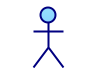
\includegraphics[height=1em]{Images/actor.png}}  % Ícono de usuario
\newcommand{\UCsystem}{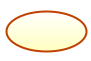
\includegraphics[height=1em]{Images/usecase.png}} % Ícono de sistema

\usepackage{etoolbox}
\makeatletter
\patchcmd{\LT@makecaption}
  {\hrule}
  {}
  {}{}
\makeatother


% Title Page
\title{Tema de tesis}
\author{Estudiante}


\begin{document}
	%Modificaciones para los nombres de algunos títulos
	\renewcommand{\listtablename}{{Índice de tablas}}
	\renewcommand{\tablename}{Tabla}
%	\renewcommand{\algorithmcfname}{Algoritmo}
	
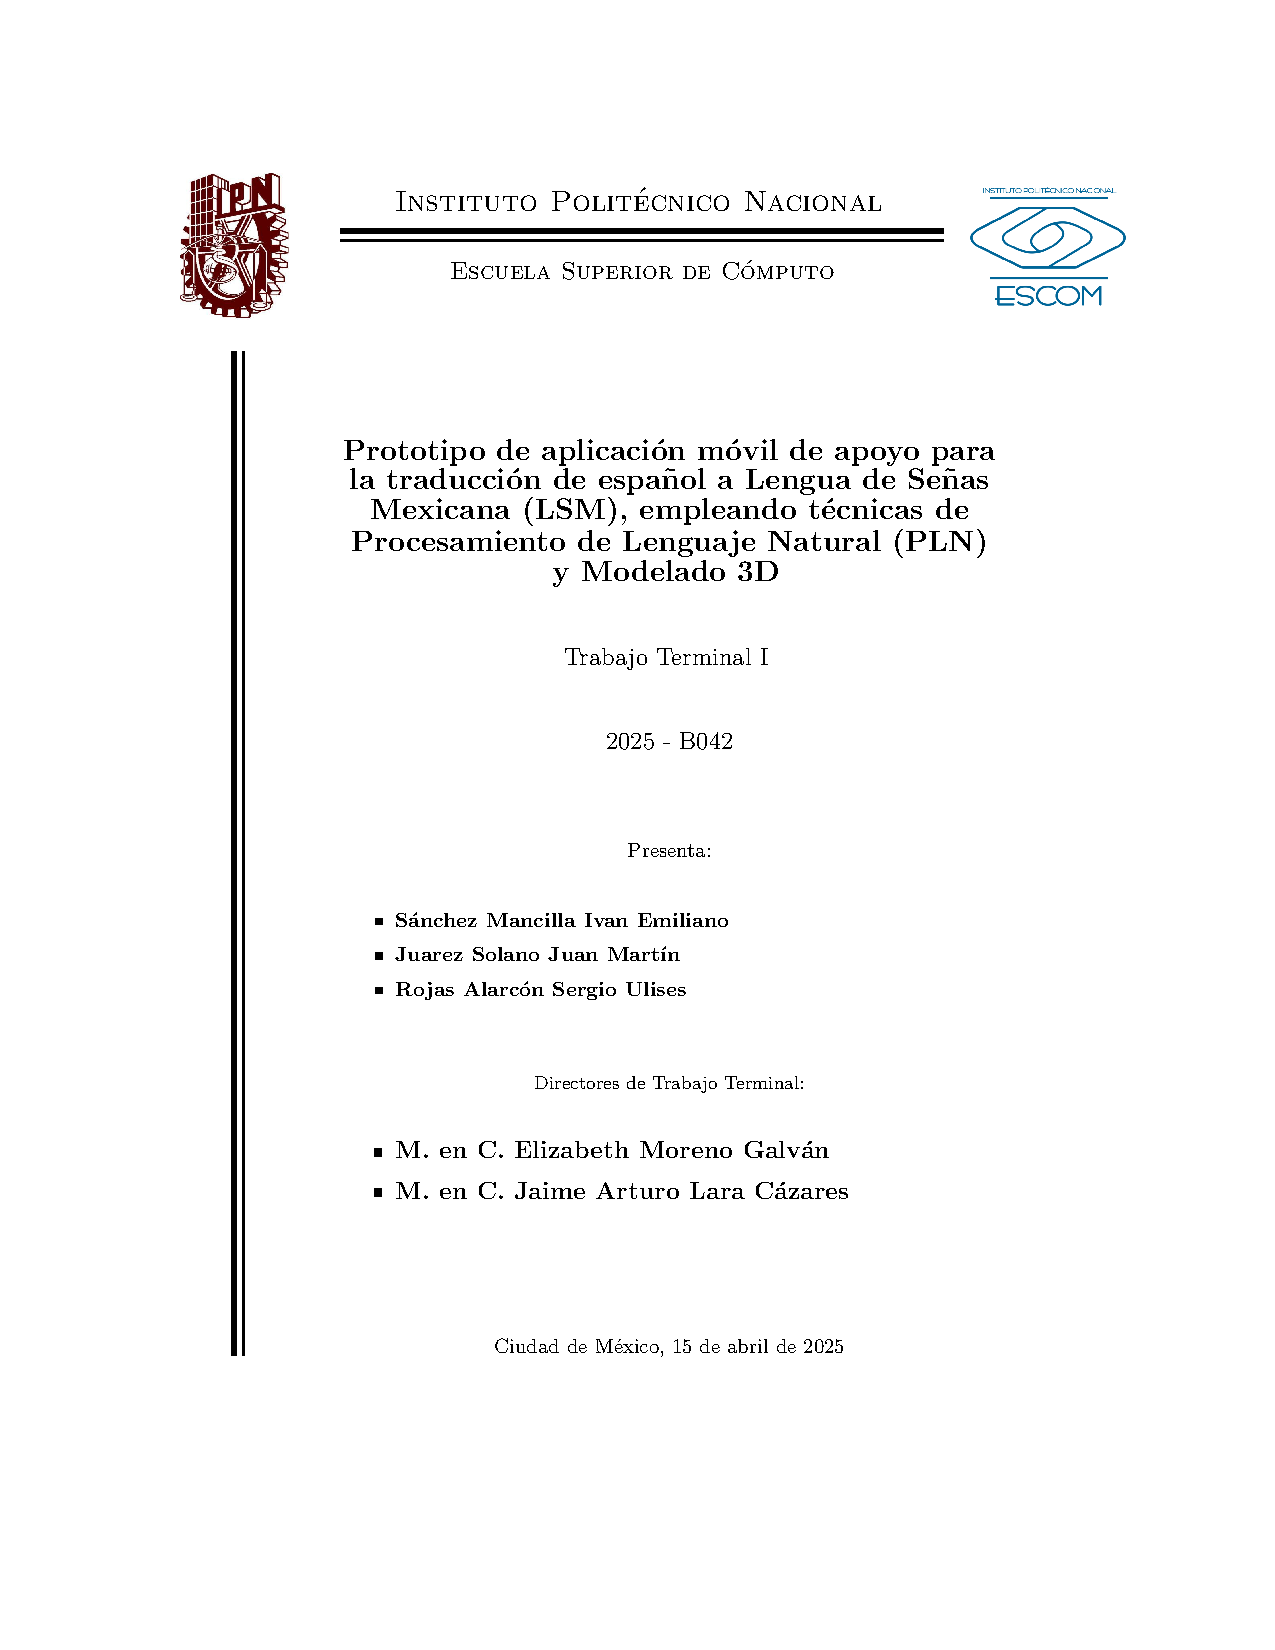
\includepdf[pages={1}]{portada}
	
%\maketitle
\section*{Resumen}
\section*{Abstract}
\newpage\null\thispagestyle{empty}\newpage

\addtocontents{toc}{\hfill \textbf{Página} \par}
\tableofcontents


% \let\cleardoublepage\clearpage
\chapter{Introducción}
\section{Motivación}
En México la comunicación es un derecho fundamental para todas las personas, ya que mediante ella se pueden establecer vínculos, e intercambiar información y pensamientos. Sin embargo, las personas de la comunidad sorda enfrentan barreras para poder comunicarse de manera efectiva. \\

Si bien la Lengua de Señas Mexicana (LSM) es el principal medio de comunicación para las personas con discapacidad auditiva en México en interacciones cotidianas o en situaciones de emergencia, las personas dependen de soluciones tecnológicas para poder comunicarse. Existen pocas herramientas digitales que permiten la traducción de español a LSM, pero en su mayoría no son precisas, y en el caso de las que emplean animaciones 3D, las mismas se muestran fragmentadas causando que se dificulte la comprensión de los mensajes.\\

La motivación de este Trabajo Terminal es mejorar la accesibilidad de las personas sordas, a la par que se fomenta la inclusión social y tecnológica para esta comunidad, empleando técnicas de Inteligencia Artificial, Procesamiento de Lenguaje Natural y Modelado 3D para obtener una traducción más fluida y natural.\\

\section{Problemática}
La comunicación es una habilidad fundamental que permite a los seres humanos poder interactuar con su entorno y compartir ideas a través de un sistema de símbolos [1]. No obstante, a menudo existen barreras en la comunicación que limitan el acceso a la información y dificultan la capacidad de las personas para poder expresarse y comunicarse [2]. \\

A pesar de las barreras, las personas sordas han desarrollado su propio medio de comunicación que les permite superar las limitaciones fisiológicas y establecer una conexión efectiva con quienes comparten este lenguaje. En el caso de México, la LSM es el principal medio de comunicación para las personas sordas en el país, con un estimado de 2.3 millones personas que padecen de esta discapacidad [3], lo que evidencia la magnitud de la población que depende de este lenguaje para poder llevar a cabo el proceso de comunicación. Esta lengua posee su propia sintaxis, gramática, léxico y está compuesta por una combinación de señas, expresiones faciales y movimientos corporales que permiten transmitir ideas, mensajes, emociones y sentimientos [4].\\

La Ley General para la Inclusión de las Personas con Discapacidad establece que los medios de comunicación deben implementar tecnologías o intérpretes de Lengua de Señas Mexicana para facilitar el acceso a contenido para la comunidad sorda [4]. En este contexto, las ciencias de la computación enfrentan un reto importante en cuanto a la creación de recursos digitales que respondan a estas necesidades específicas de accesibilidad e inclusión, concretamente en tareas de procesamiento de lenguaje y traducción automática.\\

Actualmente existen diversos proyectos relacionados con la traducción de Lengua de Señas, sin embargo, la mayoría presentan limitaciones significativas. Una de las principales dificultades es la falta de fluidez en las animaciones de la traducción del español a LSM, ya que los traductores actuales no logran representar el lenguaje de señas de manera continua, Como resultado, las animaciones suelen presentar cortes entre palabras o frases, lo que resulta en una traducción fragmentada y poco natural.\\

Estas deficiencias afectan la comprensión de los mensajes por parte de los usuarios, ya que la secuencia de señas no fluye con la rapidez y precisión necesarias para facilitar una comunicación efectiva. Además, algunos de estos proyectos están diseñados para versiones anteriores de Android y no funcionan en las versiones más recientes del sistema operativo.\\


\section{Objetivos}
\subsection{Objetivo General}
Desarrollar un prototipo de aplicación móvil en Android que, utilizando técnicas de Procesamiento de Lenguaje Natural y Modelado 3D, traduzca oraciones específicas empleadas en situaciones de emergencia, así como expresiones cotidianas como saludos y agradecimientos, del español a la Lengua de Señas Mexicana (LSM).

\subsection{Objetivo Especifícos}
\begin{itemize}
 \item Desarrollar el módulo de procesamiento de texto mediante técnicas de procesamiento de lenguaje natural, para interpretar oraciones específicas en español y transformarlas en sentencias manipulables para la traducción a la Lengua de Señas Mexicana (LSM).
    \item Construir un módulo de animación 3D que represente visualmente las señas en Lenguaje de Señas Mexicana (LSM), a partir de las oraciones procesadas.
    \item Implementar el módulo de animación 3D utilizando Inteligencia Artificial, con el fin de optimizar significativamente la fluidez entre las señas, buscando obtener una representación fluida del lenguaje de señas en los avatares.
    \item Crear una aplicación móvil en Android que integre los módulos de procesamiento de lenguaje natural, módulo de generación de animaciones 3D y transiciones fluidas entre los componentes del prototipo.
    \item Validar la funcionalidad y usabilidad de la aplicación móvil mediante pruebas con personas con discapacidad auditiva y personas oyentes, en escenarios simulados de emergencia, evaluando la precisión de la traducción y la fluidez de las animaciones.
\end{itemize}

\section{Alcance}
\subsection{Alcance Genral}
El Trabajo Terminal consiste en el desarrollo de un prototipo de aplicación móvil que traduzca frases de español a LSM mediante animaciones 3D. La aplicación tendrá un conjunto predefinido de frases comunes para saludos y situaciones de emergencia, y en caso de no contar con una frase específica, se empleará la dactilología (representación de las letras de una palabra empleando las manos) para poder garantizar la comunicación.

\subsection{Alcance Especifíco}
Se hará uso de una interfaz de usuario simple e intuitiva, que sea de utilidad para la población objetivo. Mediante técnicas de Procesamiento de Lenguaje Natural (PLN) se pretende hacer un procesamiento del dataset que contiene las frases en español, para posteriormente realizar el modelado de las animaciones 3D empleando Mediapipe; dichas animaciones serán fluidas para mostrar una comunicación natural y fácil de entender.

\subsection{Delimitación}
Es importante aclarar que la traducción será únicamente de un canal de comunicación: de español a LSM. Lo anterior por la razón de que la traducción de LSM a español es más compleja por las diferencias estructurales y gramaticales entre ambos lenguajes.\\

\section{Justificación}
En México la comunicación inclusiva es un reto para las personas con discapacidad auditiva, debido a que la mayoría de la población no conoce la Lengua de Señas Mexicana (LSM), lo que condiciona a la comunidad sorda para poder expresar sus ideas y pensamientos, acceder a servicios esenciales o recibir apoyo en situaciones de emergencia. Pese a que ha habido avances tecnológicos a lo largo de los últimos años, las herramientas de traducción de español a LSM existentes presentan limitaciones, siendo las más importantes la falta de fluidez en las animaciones y la incompatibilidad entre versiones del sistema operativo de Android. \\

Este Trabajo Terminal busca desarrollar un prototipo de aplicación móvil que traduzca frases en español a LSM con animaciones en 3D fluidas, empleando técnicas de PLN y modelado 3D. Al mejorar la calidad de la comunicación entre personas oyentes y personas con discapacidad auditiva, se contribuye a la accesibilidad, a eliminar barreras de comunicación y fomentar la comunicación inclusiva.\\

Se espera que este desarrollo sirva de referencia para sentar las bases de futuras investigaciones relacionadas a la traducción e interpretación de lenguas de señas empleando técnicas de Inteligencia Artificial (IA).\\

\section{Propuesta de solución}
Este proyecto consiste en desarrollar un prototipo que aborde las cuestiones planteadas en el apartado de la problemática, con un enfoque en mejorar la fluidez y precisión de las animaciones de LSM mediante el uso de la Inteligencia Artificial. La aplicación busca facilitar la interacción entre personas oyentes y personas con discapacidad auditiva, integrando técnicas de procesamiento de lenguaje natural y modelado 3D.\\

El traductor estará enfocado en un conjunto limitado de frases predefinidas, como expresiones de emergencia, saludos y agradecimientos. En caso de no encontrar la frase deseada, el sistema utilizará el alfabeto dactilológico de LSM para deletrear la palabra o frase, asegurando siempre una respuesta en la comunicación.\\

El uso de aplicaciones de Procesamiento de Lenguaje Natural (PLN) es fundamental para el procesamiento del español a LSM, ya que permitirá que el sistema no solo reconozca palabras aisladas, sino también frases y oraciones completas, adaptando la traducción al contexto y mejorando la comunicación en situaciones más complejas.\\

El prototipo estará diseñado para la última versión de Android, debido a que este es el sistema operativo más utilizado en México [5], por lo que la solución propuesta tendrá un mayor alcance y beneficiará a una mayor cantidad de usuarios. De acuerdo con el Instituto Federal de Telecomunicaciones (IFT), el sistema operativo más utilizado por las personas en México es Android con 84.6\%, a comparación de iOS que es utilizado por el 6.8\% [s82].\\

Para el desarrollo del prototipo se utilizará Media Pipe [6], una biblioteca eficiente para procesamiento de gestos y movimientos corporales, ideal para capturar de manera precisa los gestos de la Lengua de Señas Mexicana. Esto permitirá obtener datos precisos de las señas, garantizando una traducción más confiable y fluida, mientras se mantiene un rendimiento óptimo incluso en dispositivos de gama media.\\

Finalmente, se busca crear representaciones visuales en 3D para poder facilitar la visualización de señas. Las personas con discapacidad auditiva podrán visualizar una animación asociada a una de las frases que están incluidas dentro del prototipo.
\newline

\textbf{Productos Esperados}
\begin{itemize}
    \item Dataset normalizado de LSM.
    \item Set de animaciones con avatares 3D fluidos e interactivos.
    \item Aplicación móvil en Android.
    \item Documentación del sistema.
\end{itemize}
\begin{center}
    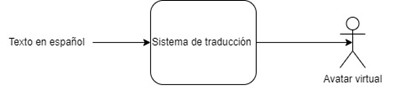
\includegraphics[width=0.8\textwidth]{Images/diacajanegra.jpg}
    \captionof{figure}{Diagrama del funcionamiento de la App, elaboración propia.}  % Pie de foto manual
\end{center}


\section{Estado del arte}
Se han desarrollado diversas investigaciones y desarrollos de sistemas de software que abordan la problemática de la comunicación entre personas oyentes y no oyentes. A continuación se describen los trabajos relacionados: 
\begin{itemize}
    \item Translation of Spanish Text to Mexican Sign Language Glossed Text Using Rules and Deep Learning. En este trabajo se presenta una arquitectura para traducir de español a Lengua de Señas Mexicana (LSM), cuyos resultados fueron evaluados con las métricas BLEU y WER. En este artículo se encontró que la traducción con técnicas tradicionales tiene un mejor desempeño que el aprendizaje profundo [7].
\item Resource Creation for Automatic Translation System from Texts in Spanish into Mexican Sign Language. Este artículo presenta la creación de recursos lingüísticos para la traducción automática del español escrito a LSM, así como el sistema que la implementa. En colaboración con la Casa de la Cultura de los Sordos (CDMX), se tradujeron 150 oraciones pertenecientes a 13 estructuras gramaticales reconocidas por el sistema, identificando 100 signos que pueden representar una oración completa. Se observó que, ante la falta de un signo específico, las personas sordas tienden a deletrear la palabra. El sistema traduce de forma literal al buscar y reproducir palabras en su base de datos, además de contar con signos que representan expresiones completas [8].
\item Aplicación “Voz y Señas”. Esta aplicación, desarrollada por el Instituto de Pedagogia en conjunto con TecnoPrótesis y Bienestar Incluyente A.C.,  permite traducir la LSM por medio del habla o escribiendo texto. Sus objetivos son favorecer la comunicación entre una persona sorda y una persona oyente, y ser una herramienta auxiliar en los procesos de alfabetización, redacción de textos y comprensión lectora [9]. 
\item Hetah. Servicio en línea que funciona como traductor de Lengua de Señas Colombiana (LSC), que permite la comunicación entre personas oyentes y no oyentes mediante un Avatar 3D. Se debe ingresar la frase que se desea traducir y posteriormente, el avatar realizará la traducción mediante gestos [10]. 
\item SignAloud. Sistema de Inteligencia Artificial que emplea guantes capaces de reconocer gestos de las manos correspondientes a palabras y frases en Lenguaje de Señas Americana. Dichos guantes contienen sensores que registran la posición y el movimiento de las manos, para generar datos que son enviados de forma inalámbrica a una computadora central. La computadora analiza los datos de los gestos empleando redes neuronales, y si los datos coinciden con un gesto, la palabra o frase asociada se pronuncia en un altavoz [11].
\item Sistema traductor de la Lengua de Señas Mexicana mediante dactilología y de español a español signado. Sistema de Inteligencia Artificial capaz de ayudar a entablar un diálogo entre una persona sorda y otra oyente, mediante la traducción de las señas de dactilología a  texto plano en español y de forma análoga, la traducción del texto plano a español a español signado [12].

	

\end{itemize}

\section{Metodología}
El proyecto se desarrollará bajo la metodología Scrum, un marco de trabajo ágil que organiza la colaboración del equipo a través de roles, artefactos y reglas que garantizan su correcta implementación [13][14]. Uno de sus principios clave es la configuración de equipos autogestionados y multifuncionales, lo que permite tomar decisiones autónomas sin depender de directrices externas [14].\\

La estructura de Scrum se basa en ciclos iterativos llamados Sprints, en los cuales se genera un incremento funcional del producto. Cada Sprint se gestiona como un proyecto independiente con objetivos específicos [14]. Además, estos ciclos incluyen cinco elementos clave: reunión de planeación, Daily Scrum, trabajo de desarrollo, revisión del Sprint y retrospectiva del Sprint, asegurando así una mejora continua en cada iteración. Para este desarrollo, los Sprints tendrán una duración de entre dos y cuatro semanas, lo que facilitará una transición progresiva hacia esta metodología y garantizará un avance constante.\\

Otro punto a destacar es que Scrum define tres roles esenciales. En primer lugar, el Scrum Master guía la implementación de la metodología y facilita la resolución de impedimentos sin gestionar directamente el desarrollo [15]. En segundo lugar, el Product Owner representa a los interesados y gestiona el Product Backlog, priorizando las funcionalidades para maximizar el valor del producto [15]. Por último, el equipo de desarrollo transforma estos requerimientos en incrementos funcionales, operando sin jerarquías y con un tamaño ideal de tres a nueve integrantes [15].\\

En este proyecto, el equipo asumirá exclusivamente el rol de desarrolladores, encargándose de transformar los requerimientos en incrementos funcionales del producto. La estructura del equipo se distribuirá en tres áreas especializadas. El desarrollador de animaciones 3D y MediaPipe diseñará avatares, implementará gestos y optimizará las transiciones. El desarrollador de Android estructurará la aplicación, desarrollará interfaces y conectará los módulos. Por su parte, el desarrollador de PLN implementará el procesamiento de lenguaje natural, adaptará las frases al contexto de LSM y optimizará la comunicación con los módulos de animación.\\

Esta distribución permitirá aplicar Scrum de manera eficiente, asegurando un desarrollo iterativo y coordinado, en el que cada integrante contribuirá activamente al avance del proyecto mediante la integración de sus respectivas áreas.


\begin{center}
    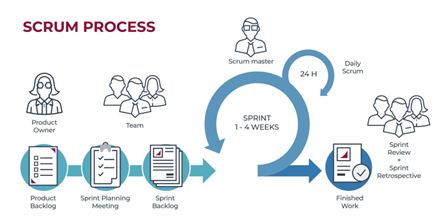
\includegraphics[width=0.8\textwidth]{Images/metoscrum.png}
    \captionof{figure}{Metodología Scrum, obtenido de [].}  % Pie de foto manual
\end{center}

\chapter{Marco Teórico: conceptos teóricos}
\section{Comunicación}
La comunicación es un proceso dinámico, en el que participa una fuente o emisor que envía un mensaje a través de un canal o medio a un potencial receptor que, a su vez, puede convertirse también en emisor [16]. Cuando se transmite el mensaje de una forma clara y efectiva para el receptor sin generar dudas ni confusiones, se logra un comunicación efectiva [17].\\

Comunicar es el acto que permite establecer relaciones efectivas, compartir experiencias, experimentar emociones y sentimientos, así como hacer que los demás lo experimenten [18].

\subsection{Tipos de Comunicación}
Uno de los tipos de comunicación está basado en si se usan palabras o no, es decir, comunicación verbal o no verbal [20]:
\begin{itemize}
    \item Comunicación verbal: se emplean palabras, y se lleva a cabo a través del habla o de manera escrita.
\item Comunicación no verbal: se emplea el lenguaje corporal, gestos, signos no lingüísticos y sonidos que no forman palabras.
\end{itemize}
Otro de los tipos de comunicación son la formal y la informan, las cuales se describen a continuación:

\begin{itemize}

\item Formal: se utiliza un lenguaje especializado y estandarizado, sin errores ni coloquialismos, además de que se toman en cuenta las jerarquías sociales.
\item Informal: no se emplea lenguaje estandarizado, no se siguen protocolos jerárquicos y se emplean coloquialismos.
\end{itemize}
Un tercer tipo de clasificación es aquella que está basada en el tipo de acto comunicativo, la cual contiene los siguientes elementos [20]:
\begin{itemize}
\item Comunicación intrapersonal: conversaciones que un ser humano entabla consigo mismo.
\item Comunicación interpersonal: intercambio de ideas y pensamientos entre dos personas, la cuál debe ser directa e interactiva.
\item Comunicación grupal: intercambio de ideas y pensamientos entre un grupo de más de dos personas, las cuales se comunican con un propósito.
\item Comunicación masiva: comunicación dirigida a un gran número de personas, mediante un medio masivo de comunicación como lo puede ser las redes sociales, radio, televisión, entre otros.
\end{itemize}

\subsection{Elementos de la comunicación}
Dentro del proceso de comunicación hay una serie de elementos que hacen posible la transmisión de un mensaje. A continuación, se enlistan cada uno de ellos: 
\begin{itemize}
    
\item Emisor. El emisor es el individuo que inicia el intercambio de información al transmitir el mensaje [18]. Dicho mensaje debe ser codificado en un sistema de símbolos que deberá ser entendible para el receptor. 

\item Receptor. Individuo que recibe el mensaje enviado, el cual es interpretado con base en las experiencias, opiniones, contexto y situación del receptor [16]. El receptor también puede ser el emisor.

\item Código. Es el sistema de signos que es empleado tanto por el emisor como por el receptor para llevar a cabo el proceso de comunicación. Ese sistema debe ser conocido por ambos para facilitar la codificación y descodificación [20].

\item Mensaje. Es la información que el emisor transmite al receptor por medio del código [19].

\item Canal. El canal es el medio en el que los mensajes del emisor se transmiten hacia el receptor [16].

\item Contexto. Se refiere a la situación en la que se lleva a cabo el proceso de comunicación, la cual tiene influencia directa en el entendimiento e interpretación del mensaje [19].

\item Retroalimentación. Es la respuesta que el receptor emite tras haber recibido e interpretado un mensaje, convirtiéndose momentáneamente en emisor. Este elemento permite cerrar el ciclo comunicativo al brindar al emisor una señal clara sobre si su mensaje fue comprendido, aceptado o necesita ser aclarado o reformulado [20].

\item Ruido o interferencia. Dentro del proceso de comunicación puede haber factores externos que dificultan o impiden el entendimiento de los mensajes [20].
\end{itemize}

\begin{center}
    \includegraphics[width=0.8\textwidth]{Images/Cap 2/ProcesoComunicación.png}
    \captionof{figure}[Proceso de comunicación]{Proceso de comunicación, elaboración propia.} 
\end{center}

La comunicación es un proceso indispensable para la interacción humana ya que por medio de ella las personas pueden intercambiar ideas, pensamientos y emociones. No obstante, como se menciona en el concepto de ruido, en ocasiones hay elementos que impiden que la comunicación se lleve a cabo, como lo pueden ser las barreras de la comunicación.
\subsection{Barreras de la comunicación}
Las barreras de la comunicación son elementos que limitan o dificultan que las personas puedan comunicarse, a la par que se dificulta su proceso de comunicación [2]. Son todas las perturbaciones que sufre un mensaje, en cualquiera de los elementos que forman parte del proceso de comunicación.

Los principales tipos de barreras son:
\begin{enumerate}
    \item \textbf{Barreras físicas.} Son interferencias causadas por elementos del entorno o en el medio donde se lleva a cabo la comunicación [21].
    \item \textbf{Barreras psicológicas.} Son aquellas que surgen por emociones, prejuicios o estados mentales que afectan la interpretación del mensaje [21].
    \item \textbf{Barreras semánticas.} Surgen cuando hay confusión en el significado de las palabras, debido a una interpretación incorrecta del lenguaje. Generalmente ocurren cuando se habla en un idioma que el emisor o el receptor no entienden, o se emplean conceptos técnicos desconocidos [21].
    \item \textbf{Barreras administrativas.} Generalmente se presentan en entornos laborales y son causadas por falta de planeación, malentendidos, falta de claridad en los procesos de comunicación y distorsiones semánticas [21].
    \item \textbf{Barreras culturales.} Este tipo de barreras se presentan cuando hay diferencias en costumbres, valores, normas o expresiones entre culturas, que imposibilitan la comunicación [21].
    \item \textbf{Barreras interpersonales.} Hace referencia a las barreras en las que hay suposiciones incorrectas y diferentes percepciones [21].
    \item \textbf{Barreras tecnológicas.} Fallas y limitaciones que se presentan en medios tecnológicos empleados para la comunicación [21].
    \item \textbf{Barreras fisiológicas.} Impedimentos físicos o biológicos causados por deficiencias en los sentidos, enfermedades o condiciones médicas que afectan cualquiera de los sentidos de manera parcial o total, afectando la transmisión de información [21]. Por ejemplo, voz débil, pronunciación defectuosa, sordera, problemas del habla, problemas visuales, etc.
\end{enumerate}
Para efectos de este Trabajo Terminal se analizarán las barreras fisiológicas, concretamente las que son causadas por problemas de sordera. En el siguiente apartado se describen los términos correctos para referirse a las personas con capacidad de escucha y a las personas con discapacidad auditiva.\\

\section{Personas con discapacidad auditiva}
\subsection{Personas Oyentes}
Un oyente se define como aquella persona con la capacidad de escuchar sonidos que le permiten interpretar mensajes. El término procede del verbo oír, que refiere a la capacidad que posee un individuo para poder percibir sonidos [22].

\subsection{Personas con discapacidad auditiva (sordas)}
Por otro lado, una persona que padece de discapacidad auditiva es aquella que ha sufrido la pérdida de la función del sistema auditivo, teniendo como consecuencia una discapacidad para poder oír, lo que dificulta el acceso al lenguaje oral [s1].\\ 

De acuerdo con la Federación Mundial de Sordos, existen aproximadamente 70 millones de personas sordas en todo el mundo, las cuales emplean más de 300 diferentes lenguas de señas [s2]. Las lenguas de señas varían entre países, presentando cambios principalmente en la estructura gramatical, sintaxis, vocabulario, signos, alfabeto y expresiones corporales [22].\\

Por otro lado, la Secretaría de Salud menciona que en México hay aproximadamente 2.3 millones de personas con discapacidad auditiva, de las cuales más del 50\% son mayores de 60 años, 34\% tienen entre 30 y 59 años, y el 2\% son niñas y niños [3].\\

Las principales causas de problemas de audición son antecedentes familiares de sordera heredados, edad avanzada, enfermedades infecciosas, exposición continua a sonidos intensos, entre otras [3].\\

Las personas sordas enfrentan consecuencias en ámbitos académicos, laborales, sociales y emocionales, debido a que las situaciones de aislamiento, deficiencia en la comunicación y dificultades del día a día repercuten negativamente para integrarse en grupos y para socializar [s21]. \\

\subsection{Tipos de Discapacidad Auditiva}
La discapacidad auditiva se clasifica en tres tipos según distintos criterios: según la parte del oído afectada, según el grado de pérdida auditiva y según el momento en que se adquiere [s22]:\\
\newline\textbf{Según la parte del oído afectada}
\begin{itemize}
    \item \textbf{Hipoacusia conductiva.} Es producida por un impedimento en el trayecto de las ondas sonoras del oído externo y medio al oído interno, causado por tumores, perforación del tímpano, traumatismos o disfunciones del oído.  
    \item \textbf{Hipoacusia neurosensorial.} Se produce cuando el nervio auditivo o las células ciliadas son dañadas, ya sea por herencia, anormalidades al momento del nacimiento, exposición a ruidos fuertes, traumatismos, entre otras causas.  
    \item \textbf{Hipoacusia mixta.} Combinación de hipoacusia conductiva e hipoacusia neurosensorial, causadas por anormalidades al nacer, infecciones, tumores y lesiones en la cabeza.  
\end{itemize}

\begin{center}
    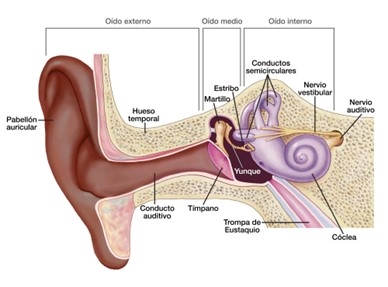
\includegraphics[width=0.9\textwidth]{Images/Cap 2/PartesOido.jpg}
    \captionof{figure}[Partes del oído humano]{Partes del oído humano, obtenido de [i2].} 
\end{center}

\textbf{Según el grado de pérdida}\\
El rango normal de audición oscila entre 0 y 20 decíbeles (dB). Tomando en consideración ese rango, se establece la siguiente clasificación de acuerdo con los dB que se hayan perdido:

\begin{itemize}
    \item \textbf{Leve:} 20-40 dB.  
    \item \textbf{Moderada:} 40-70 dB.  
    \item \textbf{Severa:} 70-90 dB.  
    \item \textbf{Profunda:} más de 90 dB.  
\end{itemize}

\textbf{Según el momento de la adquisición}\\
En esta clasificación, la discapacidad auditiva puede ser:

\begin{itemize}
    \item \textbf{Hereditaria.} La discapacidad está contenida en algunos de los genes de uno o ambos progenitores.  
    \item \textbf{Adquirida.} La discapacidad puede ser prenatal (antes del nacimiento) o postnatal (después del nacimiento), y en este último caso se deben tomar en cuenta otros criterios:
        \begin{itemize}
        \item \textbf{Prelocutiva:} antes del desarrollo del lenguaje.  
        \item \textbf{Postlocutiva:} después del desarrollo del lenguaje.  
        \end{itemize}
    \end{itemize}

Las personas sordas enfrentan consecuencias en ámbitos académicos, laborales, sociales y emocionales, debido a que las situaciones de aislamiento, deficiencia en la comunicación y dificultades del día a día repercuten negativamente para integrarse en grupos y para socializar [s21]. En la siguiente sección, se abordan las brechas entre las personas oyentes y las personas con discapacidad.

\subsection{Brechas entre personas oyentes y personas con discapacidad auditiva}
En el plano sociocultural el lenguaje es esencial en las formas de comunicación en una comunidad, pero cuando no todos los individuos pueden responder a esa lógica comunicativa se crean brechas en los discursos que giran en torno a las formas de relacionarse con los demás, puesto que aquellos que tienen códigos y configuraciones diferentes pasan a estar en un plano de invisibilidad [s24].\\

La comunidad sorda, a pesar de ser un grupo portador de un lenguaje cultural particular, debe responder a la lengua “natural” de las personas oyentes, y de no poder hacerlo ocasiona que sean excluidos en diferentes escenarios de la vida cotidiana. Esta comunidad ha sido estereotipada como personas incapaces o con limitaciones para insertarse en la sociedad, por lo que, si no pueden entrar en la “lógica natural” para comunicarse con las personas, se ven forzados a interactuar solamente con las personas que comparten su misma condición [s24].\\

A lo largo de los últimos años, se han realizado múltiples esfuerzos a nivel gubernamental y se han puesto en marcha discursos que giran alrededor del reconocimiento e inclusión de todas las personas por igual, para garantizar una mayor participación de las personas con discapacidad auditiva en escenarios sociales. No obstante, lo expresado en la legalidad dista mucho de las realidades particulares de las personas sordas en el marco sociocultural. La comunidad sorda ha sido reconocida como minoría lingüística, y por sus mismas condiciones, ha sido ubicada socialmente en el plano de la exclusión y la invisibilidad [s24]. \\ 

La presencia de barreras de comunicación generan aislamiento e impiden el desarrollo de una existencia satisfactoria, lo que puede generar graves problemas psicológicos como la depresión, ansiedad, insomnio, estrés, ideas paranoides y sensibilidad interpersonal [s1].\\

Además, la comunidad sorda presenta dificultad para acceder a la información proveniente de la televisión, radio, llamadas telefónicas, megafonías en estaciones de metro y salidas de aeropuertos, etc., debido a que esta es principalmente transmitida hacia la población oyente.\\

A pesar de que las personas sordas presentan muchas dificultades en su vida diaria, hoy en día disponen de numerosas herramientas de apoyo para impulsar su inclusión en entornos sociales y favorecer su crecimiento personal, como lo son las prótesis auditivas, señales acústicas y su propia Lengua de Señas. En este Trabajo Terminal, únicamente se centrará el estudio en las Lenguas de Señas, concretamente en la Lengua de Señas Mexicana (LSM).\\

\section{Lengua de Señas Mexicana}
\subsection{Definición de Lengua de Señas}
La lengua de señas es definida como la lengua natural de expresión y configuración gesto-espacial y percepción visual gracias a la cual los sordos pueden comunicarse con su entorno social, la cual está basada en movimientos y expresiones a través de manos, ojos, rostro, boca y cuerpo [s25].\\

En el mundo existen cerca de 300 lenguas de señas distintas, siendo así que cada país posee su propia lengua de señas. Por ejemplo, la Lengua de Señas Mexicana (LSM) es diferente a la Lengua de Señas Española (LSE), que a pesar de estar articulados en el mismo idioma (español), no comparten muchas señas en común debido a que ambas lenguas presentan señas que pueden ser regionalismos de cada país [s25].\\

Por su parte, la Lengua de Señas Mexicana (LSM) es la lengua de señas que se emplea en México, que cuenta con su propio vocabulario y gramática. A la LSM se le considera como un lenguaje por cuenta propia, debido a que es completamente capaz de expresar una amplia gama de pensamientos y emociones como cualquier otra lengua [s25].

\subsection{Lengua de Señas Mexicana (LSM)}
La Ley General para la Inclusión de las Personas con Discapacidad [s26] define a la LSM, en el Artículo 2, como la lengua de una comunidad de sordos que consiste en una serie de signos gestuales articulados con las manos y acompañados de expresiones faciales, mirada intencional y movimiento corporal, dotados de función lingüística, que forma parte del patrimonio lingüistico de dicha comunidad y es tan rica y compleja en gramática y vocabulario como cualquier lengua oral [s26].\\

Por su parte, el Artículo 20 de dicha ley establece que los medios de comunicación deben implementar la tecnología, más concretamente, de intérpretes de LSM que permitan a la comunidad de sordos las facilidades de comunicación [s26].\\

En México hay entre 87,000 y 100,000 personas hablantes de LSM que la dominan y la emplean como vía de comunicación, siendo incluso una población mucho más grande que algunas comunidades hablantes de lenguas indígenas del país [s27].\\

\subsection{Abecedario de la LSM}
La siguiente tabla explica detalladamente cómo se conforma cada una de las letras del abecedario de LSM:

\renewcommand\arraystretch{1.3}
\setlength{\fboxsep}{4pt}

\begin{longtable}{|m{2cm}|m{5cm}|m{5cm}|}
    \hline
    \textbf{Letra} & \textbf{Descripción} & \textbf{Seña} \\
    \hline
    \endfirsthead
    
    \hline
    \textbf{Letra} & \textbf{Descripción} & \textbf{Seña} \\
    \hline
    \endhead
    
    \hline
    \endfoot
    
    \hline
    \endlastfoot
    
    A & Con la mano cerrada, se muestran las uñas y se estira el dedo pulgar hacia un lado. La palma mira al frente.
    & \makecell{\colorbox{white}{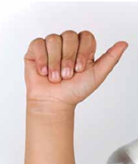
\includegraphics[width=4cm]{Images/Cap 2/Alfabeto LSM/A.png}}} \\
    \hline
    
    B & Los dedos índice, medio, anular y meñique se estiran unidos, y el pulgar se dobla hacia la palma, la cual mira al frente.
    & \makecell{\colorbox{white}{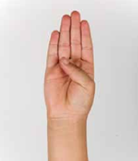
\includegraphics[width=4cm]{Images/Cap 2/Alfabeto LSM/B.png}}} \\
    \hline
    
    C & Los dedos índice, medio, anular y meñique se mantienen unidos y en posición cóncava; el pulgar también se coloca en esa posición. La palma mira a un lado.
    & \makecell{\colorbox{white}{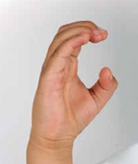
\includegraphics[width=4cm]{Images/Cap 2/Alfabeto LSM/C.png}}} \\
    \hline

    D & Los dedos medio, anular, meñique y pulgar se unen por las puntas y el dedo índice se estira. La palma mira al frente.
    & \makecell{\colorbox{white}{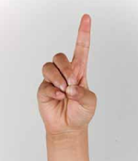
\includegraphics[width=4cm]{Images/Cap 2/Alfabeto LSM/D.png}}} \\
    \hline

    E & Se doblan los dedos completamente y se muestran las uñas. La palma mira al frente.
    & \makecell{\colorbox{white}{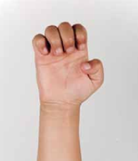
\includegraphics[width=4cm]{Images/Cap 2/Alfabeto LSM/E.png}}} \\
    \hline

    F & Con la mano abierta y los dedos unidos, se dobla el índice hasta que su parte lateral toque la yema del pulgar. La palma mira a un lado.
    & \makecell{\colorbox{white}{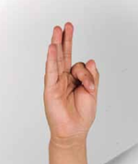
\includegraphics[width=4cm]{Images/Cap 2/Alfabeto LSM/F.png}}} \\
    \hline

    G & Se cierra la mano y los dedos índice y pulgar se estiran. La palma mira hacia la persona que se comunica.
    & \makecell{\colorbox{white}{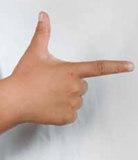
\includegraphics[width=4cm]{Images/Cap 2/Alfabeto LSM/G.png}}} \\
    \hline

    H & Se cierra la mano y los dedos índice y medio se unen y se estiran, se extiende el dedo pulgar señalando hacia arriba. La palma mira hacia la persona que se comunica.
    & \makecell{\colorbox{white}{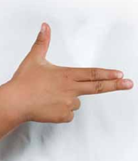
\includegraphics[width=4cm]{Images/Cap 2/Alfabeto LSM/H.png}}} \\
    \hline

    I & Con la mano cerrada, el dedo meñique se estira señalando hacia arriba. La palma se coloca de lado.
    & \makecell{\colorbox{white}{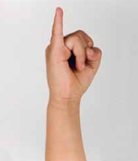
\includegraphics[width=4cm]{Images/Cap 2/Alfabeto LSM/I.png}}} \\
    \hline

    J & Con la mano cerrada, el dedo meñique estirado señala hacia arriba y la palma señala a un lado. La mano dibuja una “j” en el aire.
    & \makecell{\colorbox{white}{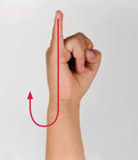
\includegraphics[width=4cm]{Images/Cap 2/Alfabeto LSM/J.png}}} \\
    \hline

    K & Se cierra la mano con los dedos índice, medio y pulgar estirados. La yema del pulgar se coloca entre el índice y el medio, moviendo la muñeca hacia arriba.
    & \makecell{\colorbox{white}{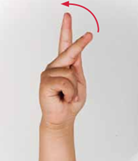
\includegraphics[width=4cm]{Images/Cap 2/Alfabeto LSM/K.png}}} \\
    \hline

    L & Con la mano cerrada y los dedos índice y pulgar estiados, se forma una “L”. La palma mira al frente.
    & \makecell{\colorbox{white}{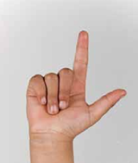
\includegraphics[width=4cm]{Images/Cap 2/Alfabeto LSM/L.png}}} \\
    \hline

    M & Con la mano cerrada, se ponen los dedos índice, medio y anular sobre el pulgar.
    & \makecell{\colorbox{white}{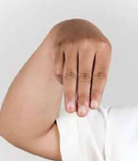
\includegraphics[width=4cm]{Images/Cap 2/Alfabeto LSM/M.png}}} \\
    \hline
 
    N & Con la mano cerrada, se ponen los dedos índice y medio sobre el pulgar. 
    & \makecell{\colorbox{white}{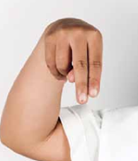
\includegraphics[width=4cm]{Images/Cap 2/Alfabeto LSM/N.png}}} \\
    \hline

    Ñ & Con la mano cerrada, se ponen los dedos índice y medio sobre el pulgar. Se mueve la muñeca a los lados. 
    & \makecell{\colorbox{white}{\includegraphics[width=4cm]{Images/Cap 2/Alfabeto LSM/Ñ.png}}} \\
    \hline

    O & Con la mano se forma una letra “o”. Todos los dedos se tocan por las puntas. 
    & \makecell{\colorbox{white}{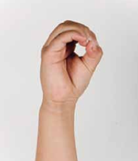
\includegraphics[width=4cm]{Images/Cap 2/Alfabeto LSM/O.png}}} \\
    \hline

    P & Con la mano cerrada y los dedos índice, medio y pulgar estirados, se coloca la yema del pulgar entre el índice y el medio.
    & \makecell{\colorbox{white}{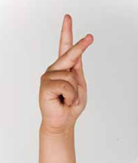
\includegraphics[width=4cm]{Images/Cap 2/Alfabeto LSM/P.png}}} \\
    \hline
    
    Q & Con la mano cerrada, se colocan los dedos índice y pulgar en posición de garra. La palma mira hacia abajo, y se mueve hacia los lados.
    & \makecell{\colorbox{white}{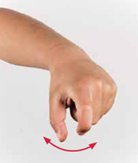
\includegraphics[width=4cm]{Images/Cap 2/Alfabeto LSM/Q.png}}} \\
    \hline
    
    R & Con la mano cerrada, se estiran y entrelazan los dedos índice y medio. La palma mira al frente.
    & \makecell{\colorbox{white}{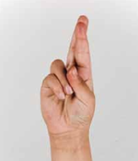
\includegraphics[width=4cm]{Images/Cap 2/Alfabeto LSM/R.png}}} \\
    \hline

    S & Con la mano cerrada, se pone el pulgar sobre los otros dedos. La palma mira al frente.
    & \makecell{\colorbox{white}{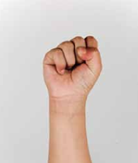
\includegraphics[width=4cm]{Images/Cap 2/Alfabeto LSM/S.png}}} \\
    \hline

    T & Con la mano cerrada, el pulgar se pone entre el índice y el medio. La palma mira al frente. 
    & \makecell{\colorbox{white}{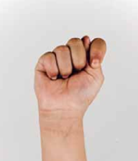
\includegraphics[width=4cm]{Images/Cap 2/Alfabeto LSM/T.png}}} \\
    \hline

    U & Con la mano cerrada, se estiran los dedos índice y medio unidos. La palma mira al frente. 
    & \makecell{\colorbox{white}{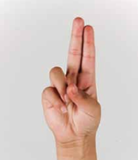
\includegraphics[width=4cm]{Images/Cap 2/Alfabeto LSM/U.png}}} \\
    \hline

    V & Con la mano cerrada, se estiran los dedos índice y medio separados. La palma mira al frente. 
    & \makecell{\colorbox{white}{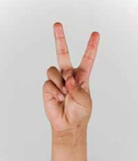
\includegraphics[width=4cm]{Images/Cap 2/Alfabeto LSM/V.png}}} \\
    \hline

    W & Con la mano cerrada, se estiran los dedos índice, medio y anular separados. La palma mira al frente. 
    & \makecell{\colorbox{white}{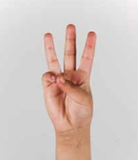
\includegraphics[width=4cm]{Images/Cap 2/Alfabeto LSM/W.png}}} \\
    \hline

    X & Con la mano cerrada, el índice y el pulgar en posición de garra y la palma dirigida a un lado, se realiza un movimiento al frente y de regreso. 
    & \makecell{\colorbox{white}{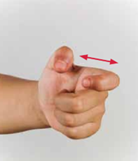
\includegraphics[width=4cm]{Images/Cap 2/Alfabeto LSM/X.png}}} \\
    \hline
    
    Y & Con la mano cerrada, se estira el meñique y el pulgar. La palma mira hacia la persona que se comunica. 
    & \makecell{\colorbox{white}{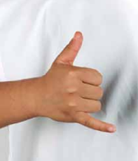
\includegraphics[width=4cm]{Images/Cap 2/Alfabeto LSM/Y.png}}} \\
    \hline

    Z & Con la mano cerrada, el dedo índice estirado y la palma al frente, se dibuja una letra z en el aire. 
    & \makecell{\colorbox{white}{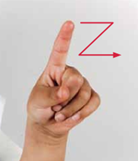
\includegraphics[width=4cm]{Images/Cap 2/Alfabeto LSM/Z.png}}} \\
    \hline
\end{longtable}
\vspace{-0.5em} % Opcional, para ajustar espacio
\captionof{table}[Abecedario de la LSM]{Abecedario de la LSM, obtenido de [s91].} \label{tabla:LSM}


\newpage

\subsection{Grámatica de la Lengua de Señas Mexicana}
La gramática estudia cómo se conectan los elementos de una lengua para crear oraciones con sentido. En la Lengua de Señas Mexicana (LSM), esa estructura no depende de sonidos ni palabras habladas, sino del uso visual del cuerpo, el espacio y los movimientos [s102].\\

La LSM se desarrolla en un espacio frente al cuerpo, dividido en tres zonas principales [s102]:

\begin{itemize}
    \item Una línea vertical que va desde la cintura hasta la parte superior de la cabeza.
    \item Un límite horizontal, que se extiende hasta los codos con los brazos en ángulo.
    \item Un tercer límite que marca qué tan lejos están las manos del cuerpo.
\end{itemize}

Si la seña se realiza fuera de estos límites, suele entenderse como un énfasis o exageración del mensaje.\\

A diferencia del español, la LSM no se basa en sonidos, sino en aspectos visuales y espaciales. Las señas suelen representar ideas complejas, como si fueran palabras individuales con sentido propio. Estas señas se consideran morfemas libres, ya que no necesitan agregarse a otras ni modificarse con terminaciones [s101].\\

En esta lengua, no se usan frecuentemente sufijos y prefijos para cambiar el significado. En su lugar, expresiones faciales, movimientos de cabeza o del cuerpo ayudan a matizar lo que se dice. Estos gestos pueden aportar información como si la acción se repite, si está terminada, si es deseada, obligatoria, o si es posible [s101].\\

Las señas no tienen una categoría gramatical fija. Una misma seña puede funcionar como verbo, adjetivo o sustantivo, dependiendo del contexto en que se use. Esta flexibilidad se debe a un fenómeno llamado prototipicidad, que permite a ciertas formas adaptarse a distintas funciones según la necesidad.\\

Existen señas que siguen patrones más estables, como los verbos direccionales, que cambian su movimiento para indicar quién realiza una acción y hacia quién va dirigida. Sin embargo, estas señas también pueden usarse en otros contextos sin perder su significado [s101].\\

Las oraciones en LSM se forman con señas que expresan acciones, participantes, tiempo, condiciones o características. En oraciones simples, las señas que representan sujetos u objetos se comportan como nombres, aunque no siempre sean sustantivos. Las acciones o ideas principales se representan con señas que funcionan como predicados [s101].\\

También es común ver señas que expresan pronombres, ubicaciones o tiempos. A veces se usa el deletreo dactilológico o nombres propios, los cuales pueden repetirse al final de la oración como una forma de remarcar la información, lo que algunos estudios llaman “etiquetado” o “tags” [s101].\\

\begin{center}
    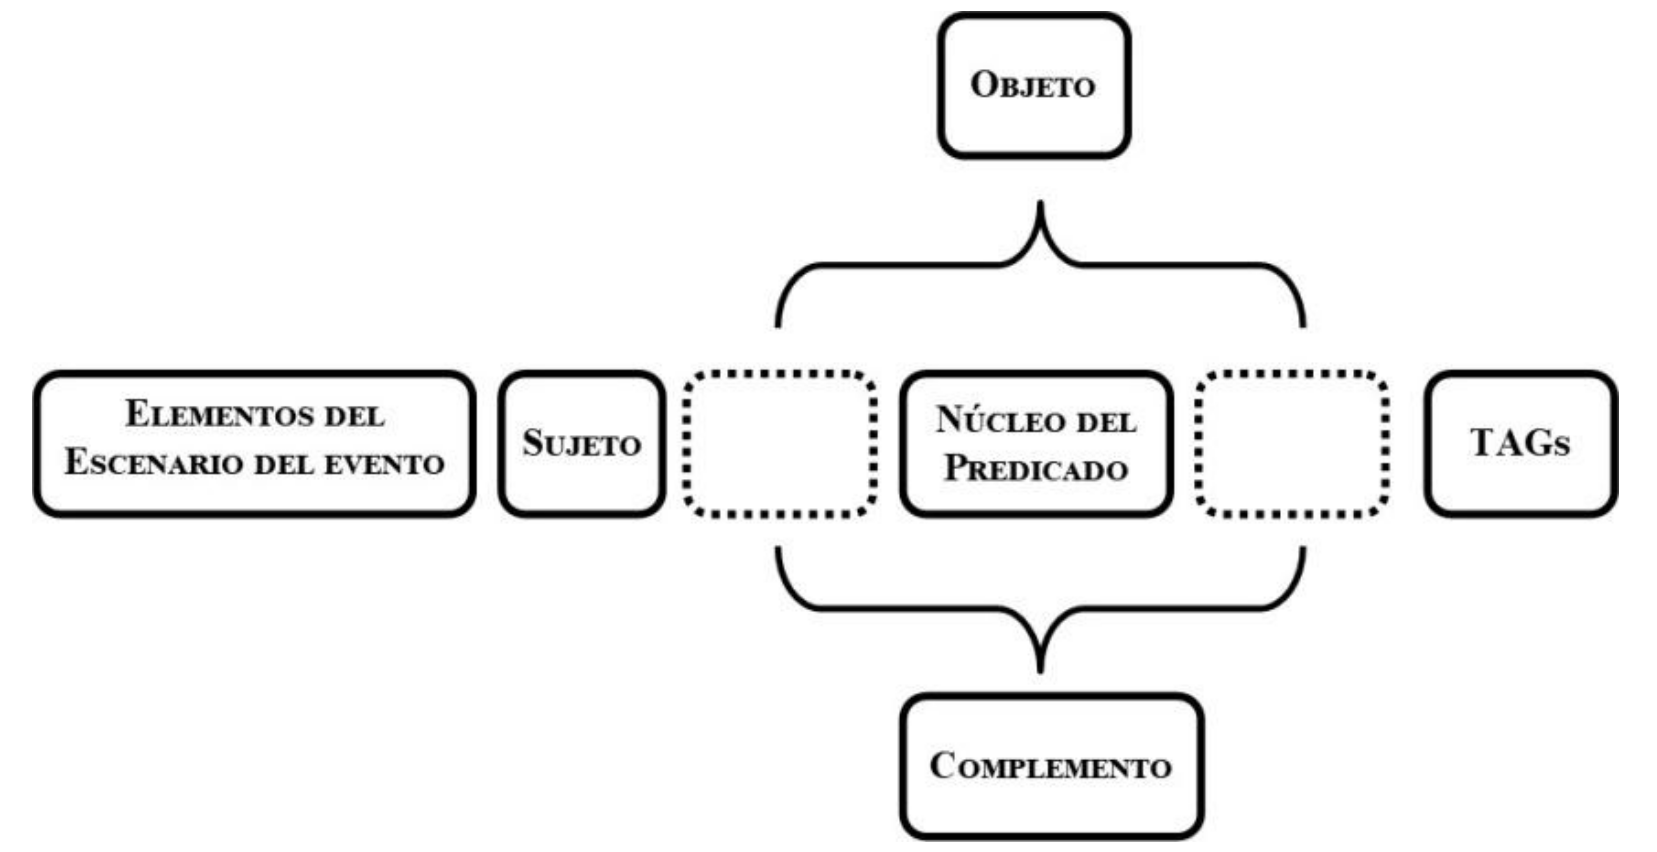
\includegraphics[width=0.9\textwidth]{Images/Cap 2/Estructura_gramatica_LSM.png}
    \captionof{figure}[Estructura gramatical de una oración de LSM]{Estructura gramatical de una oración de LSM, obtenido de [s101].}  % Pie de foto manual
\end{center}

\textbf{Fonología}\\
En las lenguas de señas, los fonemas, las unidades mínimas con significado, pueden descomponerse en siete componentes esenciales [s100]:

\begin{enumerate}
    \item Configuración manual: Es la forma específica que adopta la mano al ejecutar un signo determinado.
    \item Orientación de la mano: Hace referencia a la dirección en la que se posiciona la palma, ya sea orientada hacia arriba, abajo o frente al emisor.
    \item Zona de ejecución: Indica la parte del cuerpo en la que se realiza el signo, como por ejemplo la frente, la boca, el pecho o los hombros.
    \item Desplazamiento: Describe el tipo de movimiento que se lleva a cabo con las manos al hacer un signo; este puede ser giratorio, lineal, en vaivén o segmentado.
    \item Área de contacto: Se refiere a la parte de la mano dominante (la derecha para personas diestras o la izquierda para personas zurdas) que entra en contacto con el cuerpo. Puede involucrar la palma, las yemas o el dorso de los dedos.
    \item Plano de producción: Se trata de la distancia entre el cuerpo y el lugar donde se articula el signo. El Plano 1 está en contacto directo con el cuerpo, mientras que el Plano 4 se encuentra más alejado, con los brazos completamente extendidos.
    \item Elementos corporales no manuales: Son señales complementarias que refuerzan el mensaje, como expresiones faciales, movimientos del torso, gesticulaciones orales o el uso del cuello y los hombros. Por ejemplo, para comunicar una acción futura se inclina el cuerpo hacia delante, y para indicar el pasado, hacia atrás.\\
\end{enumerate}

\textbf{La Configuración Manual (CM) en la LSM}\\
En las lenguas de señas, las manos son las principales herramientas para comunicar, aunque no son las únicas. Además de considerar la dirección del movimiento y el lugar en el espacio donde se hace una seña, también es esencial observar la forma que toman las manos, conocida como configuración manual (CM). Esta configuración puede variar tanto en la mano dominante como en la no dominante.\\

La configuración manual, entonces, representa la forma específica que adoptan las manos al momento de hacer una seña. Esto incluye aspectos como:

\begin{itemize}
    \item La posición de los dedos: si están juntos o separados, doblados o rectos.
    \item La forma general de la mano: abierta, en puño, en forma de garra, etc.
    \item La ubicación del pulgar y del índice, que suelen tener movimientos propios.
\end{itemize}

Desde un punto de vista técnico, la configuración manual forma parte de lo que se llama la matriz articulatoria. Dentro de ella, se distinguen dos grupos importantes:

\begin{itemize}
    \item Los dedos (índice, medio, anular y meñique), que suelen moverse como bloque.
    \item El pulgar, que, por su movilidad más independiente, se analiza aparte.
\end{itemize}

Debido a todas las combinaciones posibles entre estos elementos, las configuraciones manuales no pueden reducirse a formas simples, sino que son estructuras complejas que generan significado cuando se combinan con otros componentes de la seña.

\newpage

\textbf{Orientación de la Palma de la Mano}\\
La orientación de la palma se refiere a la dirección en la que se encuentra la palma de la mano en relación con el cuerpo de la persona que está haciendo la seña, justo en el momento en que adopta la configuración manual.

En la Lengua de Señas Mexicana (LSM), se han identificado nueve posibles formas de orientar la palma durante la articulación de una seña. Estas son:

\begin{enumerate}
    \item Palma hacia arriba, con los dedos apuntando a la izquierda.
    \item Palma hacia arriba, con los dedos apuntando hacia el frente.
    \item Palma hacia abajo, con los dedos dirigidos a la izquierda.
    \item Palma hacia abajo, con los dedos apuntando hacia adelante.
    \item Palma hacia la izquierda, con los dedos hacia arriba.
    \item Palma hacia la izquierda, con los dedos hacia el frente.
    \item Palma hacia el frente, con los dedos señalando hacia arriba.
    \item Palma frente al cuerpo, dedos hacia arriba.
    \item Palma frente al cuerpo, dedos hacia la izquierda.
\end{enumerate}

\begin{center}
    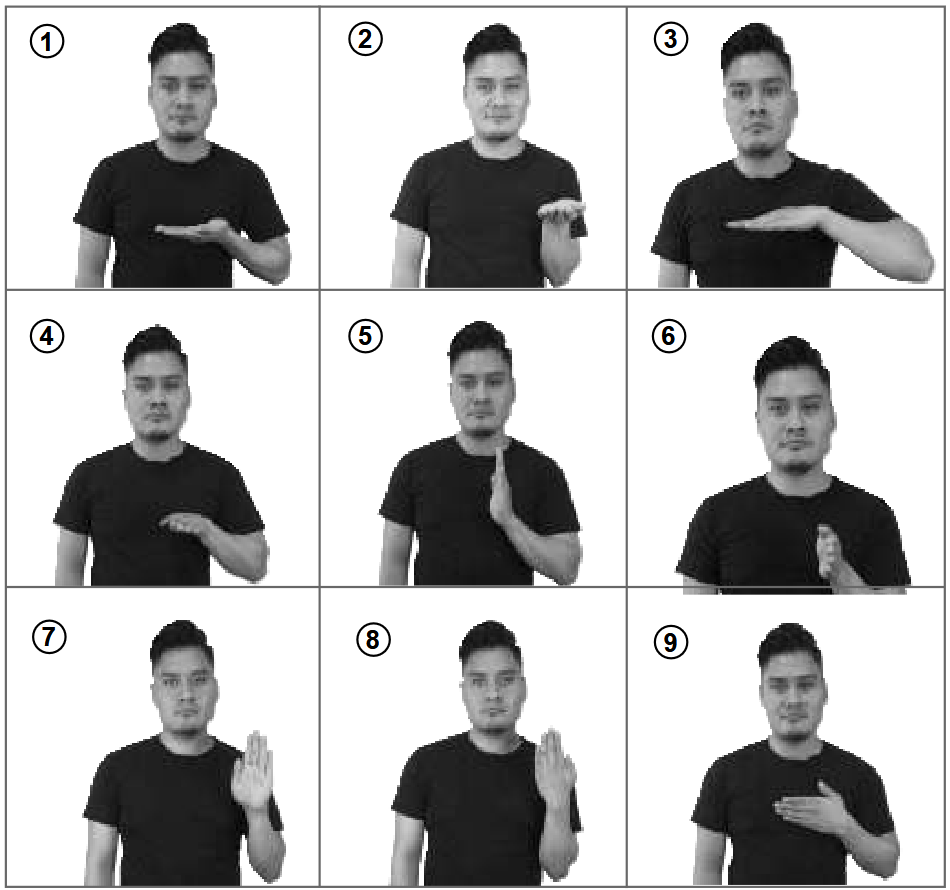
\includegraphics[width=0.7\textwidth]{Images/Cap 2/Orientacion_Palma_Mano.png}
    \captionof{figure}[Orientaciones de la palma de la mano en LSM]{Orientaciones de la palma de la mano en LSM, obtenido de [s102].}  % Pie de foto manual
\end{center}

Cada una de estas orientaciones forma parte de la estructura visual y espacial de una seña, y su correcta ejecución es clave para transmitir el significado deseado.\\

\textbf{Ubicación en la Lengua de Señas Mexicana (LSM)}\\
La ubicación se refiere al lugar específico en el espacio donde se realiza una seña. Este espacio, conocido como espacio señante, puede estar frente al cuerpo o sobre él, y es clave para transmitir el significado correcto.\\

Para describir las señas en este diccionario, se dividió el espacio señante principalmente en niveles de altura y direcciones laterales. En algunos casos, también se toma en cuenta una tercera dimensión, que implica mayor cercanía o profundidad.\\

Cuando las señas se hacen sobre el cuerpo, se habla de "alturas" específicas, como por ejemplo:
\begin{itemize}
    \item A la altura del cuello
    \item A la altura del hombro
    \item A la altura del pecho
    \item A la altura del plexo
    \item A la altura de la cintura
    \item A la altura de la cadera
\end{itemize}

Si la seña se mueve entre dos puntos, se describe como un desplazamiento, por ejemplo:

\begin{itemize}
    \item Del pecho a la cintura
    \item Del hombro a la cadera
    \item Del cuello a la cadera
\end{itemize}

Cuando el movimiento es horizontal o de un lado a otro, también se aclara, por ejemplo:
\begin{itemize}
    \item A la altura del pecho, de izquierda a derecha
\end{itemize}

En el caso de las señas realizadas en la cara, se puede ser más preciso indicando zonas como:
\begin{itemize}
    \item A la altura de los ojos
    \item A la altura de las cejas    
\end{itemize}

Y si la seña se hace sobre el tronco del cuerpo, se especifica si es:
\begin{itemize}
    \item Del lado izquierdo
    \item Del lado derecho
    \item Al centro
\end{itemize}

Aunque algunas ubicaciones pueden detallarse aún más, se busca usar una descripción unificada para facilitar la comprensión.\\

\textbf{Dirección del Movimiento de la mano en la LSM}\\
La dirección se refiere a la trayectoria que la mano sigue al realizar una seña. En el siguiente esquema se muestran las nueve direcciones que las configuraciones manuales pueden seguir durante la articulación de las señas respecto al cuerpo.

\begin{center}
    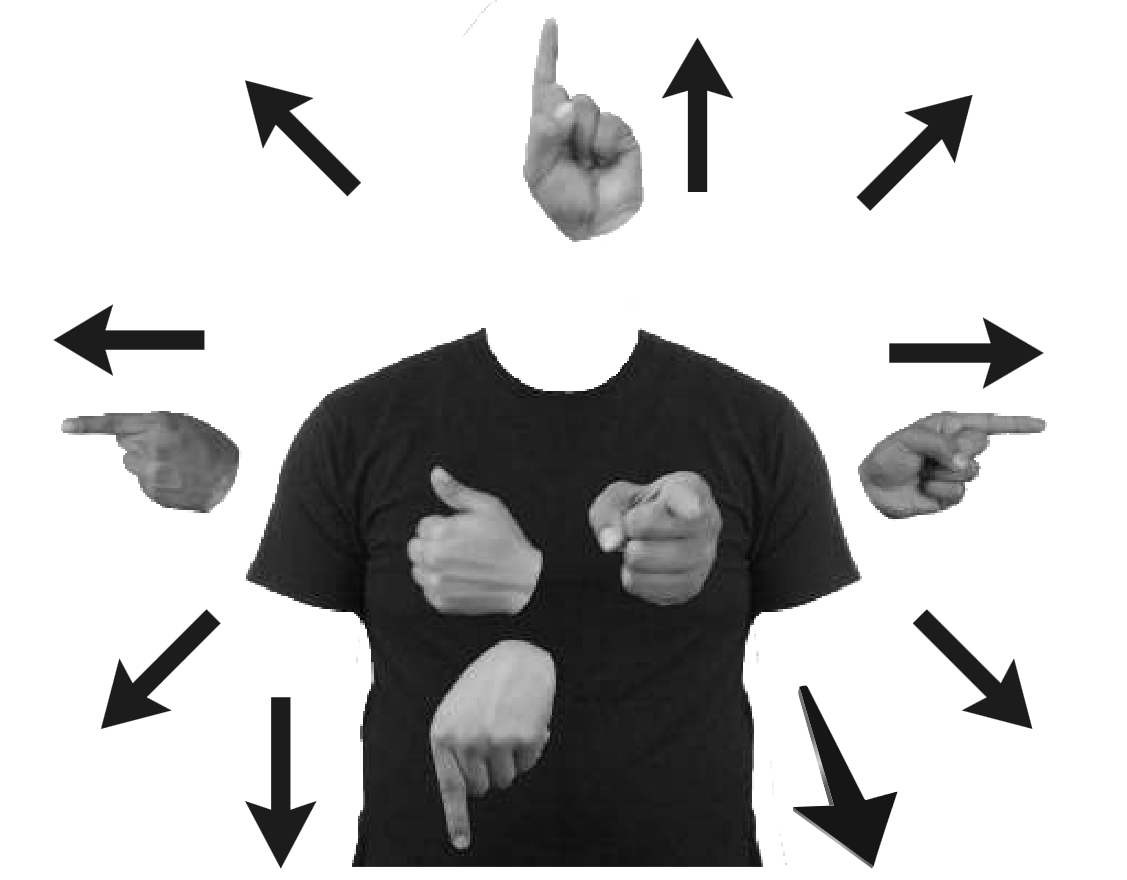
\includegraphics[width=0.8\textwidth]{Images/Cap 2/Direccion_Manos_LSM.png}
    \captionof{figure}[Direcciones posibles que sigue la mano en la LSM]{Direcciones posibles que sigue la mano en la LSM, obtenido de [s102].}  % Pie de foto manual
\end{center}

\textbf{Explicación de los movimientos y sus símbolos}\\
Una vez especificadas las posibles direcciones de las configuraciones manuales, se presenta a continuación una tabla con todos los movimientos que las manos pueden realizar en la LSM. En la primera columna se menciona el nombre del movimiento; en la segunda, la descripción del mismo, y en la tercera aparecen flechas o imágenes de la mano para indicar la dirección o la manera en que las configuraciones manuales se mueven.\\

\renewcommand\arraystretch{1.3}
\setlength{\fboxsep}{4pt}

\begin{longtable}{|m{5cm}|m{5cm}|m{5cm}|}
    \hline
    \textbf{Movimiento} & \textbf{Descripción del Movimiento} & \textbf{Imagen} \\
    \hline
    \endfirsthead
    
    \hline
    \textbf{Movimiento} & \textbf{Descripción del Movimiento} & \textbf{Imagen} \\
    \hline
    \endhead
    
    \hline
    \endfoot
    
    \hline
    \endlastfoot
    
     & Se emplea una numeración progresiva para señalar cómo cambian las formas de las manos y los desplazamientos en las señas que combinan varios movimientos.
    & \makecell{\colorbox{white}{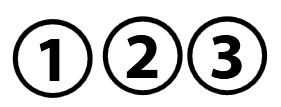
\includegraphics[width=4cm]{Images/Cap 2/Movimientos LSM/1.png}}} \\
    \hline

    Lineal (lin) & Movimiento rectilíneo.
    & \makecell{\colorbox{white}{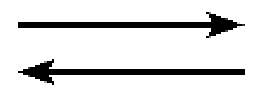
\includegraphics[width=4cm]{Images/Cap 2/Movimientos LSM/2.png}}} \\
    \hline

    Arco (ar) & El desplazamiento del brazo, la muñeca o la mano dibuja una curva en forma de arco.
    & \makecell{\colorbox{white}{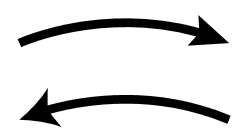
\includegraphics[width=4cm]{Images/Cap 2/Movimientos LSM/3.png}}} \\
    \hline

    Extensión de dedos (E) & Los dedos se extienden.
    & \makecell{\colorbox{white}{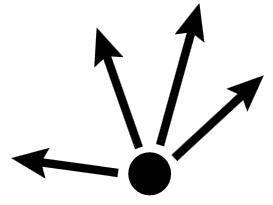
\includegraphics[width=4cm]{Images/Cap 2/Movimientos LSM/4.png}}} \\
    \hline

    Vaivén (va) & Se realiza un movimiento intercalado entre ambas manos o brazos.
    & \makecell{\colorbox{white}{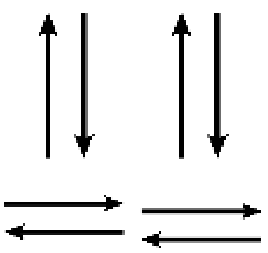
\includegraphics[width=4cm]{Images/Cap 2/Movimientos LSM/5.png}}} \\
    \hline
    
    Circular (circ) & La trayectoria de la mano, muñeca o brazo describe movimientos circulares o semicirculares.
    & \makecell{\colorbox{white}{
\includegraphics[width=4cm]{Images/Cap 2/Movimientos LSM/6.png}}} \\
    \hline

    Espiral (es) & La mano o el brazo giran siguiendo un patrón redondeado.
    & \makecell{\colorbox{white}{
\includegraphics[width=4cm]{Images/Cap 2/Movimientos LSM/7.png}}} \\
    \hline

    Flexión de dedos (f) & Los dedos se retraen.
    & \makecell{\colorbox{white}{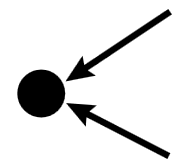
\includegraphics[width=4cm]{Images/Cap 2/Movimientos LSM/8.png}}} \\
    \hline

    Ondular (ond) & El movimiento de la mano o el brazo imita una forma de onda.
    & \makecell{\colorbox{white}{
\includegraphics[width=4cm]{Images/Cap 2/Movimientos LSM/9.png}}} \\
    \hline
    
    Salto & La mano o los dedos simulan uno o varios saltos.
    & \makecell{\colorbox{white}{
\includegraphics[width=4cm]{Images/Cap 2/Movimientos LSM/10.png}}} \\
    \hline

    Movimiento vibratorio local (vib) & La mano tiembla.
    & \makecell{\colorbox{white}{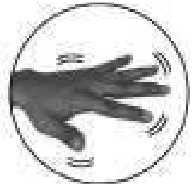
\includegraphics[width=4cm]{Images/Cap 2/Movimientos LSM/11.png}}} \\
    \hline
    
    Cabeceo de muñeca (cab) & El movimiento parte desde la parte posterior y avanza al frente, usando solo el giro de la muñeca.
    & \makecell{\colorbox{white}{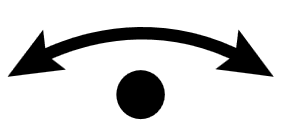
\includegraphics[width=4cm]{Images/Cap 2/Movimientos LSM/12.png}}} \\
    \hline
    
    Aplanado (apl) & Se realiza un contacto breve entre el índice y medio, o el índice y el pulgar, seguido de una separación.
    & \makecell{\colorbox{white}{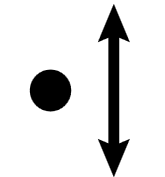
\includegraphics[width=4cm]{Images/Cap 2/Movimientos LSM/13.png}}} \\
    \hline

    Apulgarado (p) & El índice o medio se libera con impulso del pulgar, pasando de estar doblado a completamente recto.
    & \makecell{\colorbox{white}{\includegraphics[width=4cm]{Images/Cap 2/Movimientos LSM/14.png}}} \\
    \hline

    Cambios progresivos en los dedos (prog) & Los dedos se mueven uno a uno de forma intercalada.
    & \makecell{\colorbox{white}{\includegraphics[width=4cm]{Images/Cap 2/Movimientos LSM/15.png}}} \\
    \hline

    Deslizamiento (desl) & Se realiza un movimiento deslizante de los dedos sobre la superficie del pulgar.
    & \makecell{\colorbox{white}{\includegraphics[width=4cm]{Images/Cap 2/Movimientos LSM/16.png}}} \\
    \hline

    Zig-zag (zig) & El índice traza en el aire la forma de la letra Z.
    & \makecell{\colorbox{white}{\includegraphics[width=4cm]{Images/Cap 2/Movimientos LSM/17.png}}} \\
    \hline
    
    Siete (7) & Se realiza un movimiento que dibuja el número siete en el espacio.
    & \makecell{\colorbox{white}{\includegraphics[width=4cm]{Images/Cap 2/Movimientos LSM/18.png}}} \\
    \hline

    Rotación de muñeca (rot) & La rotación del antebrazo o la muñeca provoca que la mano cambie su dirección.
    & \makecell{\colorbox{white}{\includegraphics[width=4cm]{Images/Cap 2/Movimientos LSM/19.png}}} \\
    \hline
    
    Choque (ch) & Las manos se encuentran y se tocan.
    & \makecell{\colorbox{white}{\includegraphics[width=4cm]{Images/Cap 2/Movimientos LSM/20.png}}} \\
    \hline
    
    Doblar (dob) & Mientras el pulgar permanece quieto, los demás dedos se doblan hacia el centro de la mano.
    & \makecell{\colorbox{white}{\includegraphics[width=4cm]{Images/Cap 2/Movimientos LSM/21.png}}} \\
    \hline
    
    Cruzado (crz) & Los brazos se mueven hacia el centro cruzándose, y las manos se aproximan en un punto medio.
    & \makecell{\colorbox{white}{\includegraphics[width=4cm]{Images/Cap 2/Movimientos LSM/22.png}}} \\
    \hline
    
    Simétrico (sim) & Desde una posición inicial común, las manos se separan hacia diferentes direcciones: superior, inferior o lateral.
    & \makecell{\colorbox{white}{\includegraphics[width=4cm]{Images/Cap 2/Movimientos LSM/23.png}}} \\
    \hline

    Prensar & El índice y el pulgar realizan un gesto de pinza al agarrar otra mano o una zona del cuerpo.
    & \makecell{\colorbox{white}{\includegraphics[width=4cm]{Images/Cap 2/Movimientos LSM/24.png}}} \\
    \hline
\end{longtable}
\vspace{-0.5em} % Opcional, para ajustar espacio
\captionof{table}[Movimientos de las manos]{Movimientos de las manos, obtenido de [s91].} \label{tabla:Movimiento_LSM}

\textbf{Rasgos no manuales: expresión facial y gestos}\\
Los rasgos no manuales (RNM) en la Lengua de Señas Mexicana incluyen la expresión facial, los gestos y los movimientos del cuerpo. Estos elementos se realizan al mismo tiempo que las señas y tienen una función gramatical clave, ya que aportan significado al mensaje, similar a cómo el tono de voz o la velocidad lo hacen en el español hablado.\\

También existen gestos universales que no dependen del idioma o la cultura, como los que expresan felicidad, tristeza, dolor o alegría, y que se entienden en cualquier parte del mundo.\\

\textbf{Tipos de Señas en la LSM}\\
En la Lengua de Señas Mexicana (LSM), las señas se pueden clasificar de diferentes maneras, principalmente según cuántas manos se usan y cómo se mueven.

\begin{itemize}
    \item Seña manual (SM): Se realiza con una sola mano.
    \item Seña bimanual (SB): Usa ambas manos, pero no necesariamente hacen lo mismo; puede haber movimientos distintos entre una y otra.
    \item Seña simétrica (SS): Ambas manos se mueven al mismo tiempo con movimientos similares o en espejo (como si se reflejaran una a la otra).
    \item Seña compuesta (SC): Se forma a partir de dos o más señas simples o al menos tres formas diferentes de las manos.
\end{itemize}

\newpage
Además, según la relación entre la seña y su significado, también se pueden clasificar así:
\begin{itemize}
    \item Icónicas: Estas señas imitan la forma o alguna característica del objeto al que se refieren. Por ejemplo, la seña de "árbol" muestra cómo es un árbol.
    \item Referenciales en el cuerpo: Algunas señas se hacen en partes del cuerpo relacionadas con el objeto, como la seña de "manzana", que se realiza en la mejilla.
    \item Arbitrarias: No guardan ninguna relación visual con el objeto o concepto. Ejemplos de estas son las señas de "gracias" u "oportunidad".
    \item Inicializadas o alfabéticas: Se utilizan las letras del alfabeto manual, generalmente la inicial de la palabra en español, como en “mamá” o “alumno”.
    \item Indéxicas: Estas señas señalan un lugar, persona u objeto en el espacio, como los pronombres: yo, tú, él, ella, allá, aquí, etc.
    \item Numéricas: Son aquellas donde la forma de la mano representa un número, y se usan para nombrar cosas como países o acciones. Ejemplos: "Dinamarca" (con el número 8), "mujer" (número 1), "abanico" (número 4) y "atención" (número 6).\\
\end{itemize}

\textbf{Clasificadores en la LSM}\\
En la LSM, los clasificadores son señas especiales que permiten describir mejor las características de un objeto. Estas señas combinan dos elementos: uno que indica a qué tipo de objeto se hace referencia (como persona, animal, cosa) y otro que muestra sus propiedades, como forma, tamaño o cómo se mueve.\\

Los clasificadores se basan en la configuración manual (CM), es decir, en la forma en la que se colocan y usan las manos. A través de estas configuraciones, se puede representar si un objeto es redondo, plano, grande, pequeño, blando, rígido, entre otros rasgos. También se pueden indicar su ubicación, cantidad u orden. Son muy útiles cuando no existe una seña exacta para algo, y ayudan a transmitir el mensaje de manera visual y clara.\\

Además, existen clasificadores de predicado, que no solo describen el objeto, sino que también aportan información sobre su movimiento, posición o estado. Estos se combinan con “raíces de movimiento” para señalar si algo se mueve, está quieto o entra en contacto con algo. Las raíces de movimiento pueden ser:
\begin{itemize}
    \item Movimiento o proceso
    \item Descripción estática
    \item Contacto con otro objeto
\end{itemize}

Los clasificadores también se organizan en diferentes tipos, dependiendo de lo que representan:
\begin{itemize}
    \item Clasificadores de entidad (personas, animales, cosas)
    \item De superficie (planos, mesas, pisos)
    \item De profundidad y anchura (algo profundo o ancho)
    \item De extensión o límites (como bordes o extremos)
    \item De perímetro (formas cerradas)
    \item De instrumento (objetos usados para realizar acciones) 
\end{itemize}

\textbf{Afijos}\\
Un afijo es una pequeña unidad con significado que se añade a una palabra para cambiar su sentido o su función gramatical. De acuerdo con la definición de la Real Academia Española, los afijos son morfemas que se agregan a la raíz de una palabra para alterar su significado o categoría. Sin embargo, en la Lengua de Señas, el uso de afijos no es común como lo es en las lenguas orales.\\

En las lenguas habladas, los afijos como prefijos y sufijos son parte esencial de la estructura de muchas palabras. En cambio, en la Lengua de Señas, su presencia es limitada y aparece sobre todo en situaciones en las que interviene el español escrito. Generalmente, son personas oyentes que conocen la LSM quienes tienden a emplear estos elementos con mayor frecuencia, adaptando la estructura del español al sistema visual y gestual de la lengua de señas.\\

\textbf{Prefijos}\\
En la Lengua de Señas Mexicana (LSM), los prefijos son elementos que se colocan al inicio de una seña para agregar información como el tiempo, el género o el número. Aunque en las lenguas orales los prefijos son comunes, en LSM su uso es más limitado y, en muchos casos, surge por influencia del español. Actualmente, se conservan pocos prefijos, como por ejemplo “in-” o “im-”, que se representan con una “I” hecha por la mano dominante al tocar la mano base.\\

Para expresar el género femenino, se utiliza una seña específica que aparece después de indicar el masculino. El número (singular o plural) suele marcarse antes del sustantivo, y si se quiere enfatizar, puede colocarse también después.\\

El tiempo del mensaje se indica al inicio, ya sea mediante una seña específica o con movimientos del cuerpo: inclinarse hacia adelante para el futuro, o hacia atrás para el pasado.\\

En cuanto a la negación, existen señas conocidas como dobletes, que tienen una forma afirmativa y otra negativa completamente distinta, sin necesidad de añadir gestos como mover la cabeza. Algunos ejemplos son:
\begin{itemize}
    \item Gustar / No gustar
    \item Poder / No poder
    \item Saber / No saber
    \item Todavía / Todavía no
    \item Querer / No querer
    \item Haber / No haber
    \item Sirve / No sirve
\end{itemize}

\textbf{Sufijos}\\
Los sufijos son pequeñas unidades de significado que se colocan después de una seña para dar más precisión o detalle al mensaje. Su uso en la Lengua de Señas Mexicana (LSM) se ha dado principalmente por la influencia del idioma español, ya que en las lenguas orales es común agregar estas terminaciones a las palabras.\\

En el pasado, los sufijos más frecuentes en LSM eran “-ción” y “-mente”, ya que ayudan a formar sustantivos abstractos o adverbios. Sin embargo, con el tiempo han dejado de usarse tanto, y actualmente los sufijos que se siguen utilizando con mayor frecuencia son:

\begin{itemize}
    \item -ito / -ita, que indican diminutivo o cercanía con afecto.
    \item -al, usado para formar adjetivos relacionados a un lugar o cosa.
    \item -or / -ora, que hacen referencia a profesiones o a quien realiza una acción.
    \item -dad, que se usa para formar conceptos abstractos, como en “amistad” o “bondad”.
\end{itemize}

\subsection{Dactilogía}
La dactilología es un sistema de comunicación que transmite información mediante el deletreo manual, y en ocasiones es usado en conjunto con la lengua de señas. Se emplea la mano de diferente manera para pronunciar cada una de las letras [s22].\\

Otra definición de la dactilología es que es la representación manual de cada una de las letras que componen el alfabeto, para poder transmitir a las personas sordas cualquier palabra que se desee comunicar. Todas las lenguas de señas poseen mecanismos internos que les permiten generar mensajes [s23].\\

Para comunicarse por medio de dactilología se emplea la mano dominante a la altura de la barbilla, en conjunto con la articulación oral, siendo necesario que la cara y la boca sean visibles [s23]. Principalmente se usa para sustantivos, nombres propios, direcciones y palabras para los cuales no existe un signo creado.\\

Si bien la discapacidad auditiva representa una barrera de la comunicación, las personas sordas en los últimos años han buscado superar esa barrera con ayuda de dispositivos tecnológicos que puedan fungir como intérpretes. El desarrollo de la Inteligencia Artificial (IA), más concretamente las técnicas de Procesamiento de Lenguaje Natural (PLN) y modelado de animaciones 3D, han ayudado a crear nuevos sistemas que faciliten la interacción entre personas oyentes y personas de la comunidad sorda, derribando las barreras de la comunicación.\\

En los siguientes apartados se analizarán un par de herramientas que serán necesarias para el desarrollo del prototipo planteado en el capítulo 1, como lo es la Inteligencia Artificial y el Procesamiento de Lenguaje Natural.\\

\section{Inteligencia Artificial}
La Inteligencia Artificial (IA) es la capacidad que poseen las máquinas para usar algoritmos y aprender de los datos para tomar decisiones tal como lo haría un ser humano [s3]. A diferencia del ser humano, la IA no necesita descansar y es capaz de analizar grandes cantidades de información, reduciendo el margen de error.\\

La IA se basa en el uso de algoritmos y tecnologías de aprendizaje automático para dar a las máquinas la capacidad de aplicar ciertas habilidades cognitivas y realizar tareas por sí mismas de manera autónoma o semiautónoma. A medida que la IA mejora, muchos procesos son más eficientes y algunas tareas que parecían complicadas se realizan con mayor rapidez y precisión [s31].\\

\subsection{Clasificación de la Inteligencia Artificial}
La IA puede ser clasificada de varias maneras, ya sea a partir de su grado de capacidad cognitiva o a partir de su grado de autonomía [s31].\\

\textbf{Clasificación a partir de su grado de capacidad cognitiva:}
\begin{itemize}
    \item Inteligencia Artificial débil o limitada. Está diseñada para realizar tareas específicas de manera eficiente, pero no tiene la capacidad de razonar ni aprender de nuevas situaciones [s31].\\
\item Inteligencia Artificial general o fuerte. Este tipo de IA tiene la capacidad de realizar varias tareas cognitivas como el razonamiento, el aprendizaje y la resolución de problemas. A diferencia de la IA débil, la IA fuerte es capaz de adaptarse a nuevas situaciones y entornos [s31].\\
\item Super Inteligencia Artificial. Tiene la capacidad de realizar cualquier tarea compleja que requiere Inteligencia Humana, ya que es muy poderosa, y puede superar a los seres humanos en términos de capacidad cognitiva y de aprendizaje [s31].\\

\end{itemize}

\textbf{Clasificación de acuerdo con su grado de autonomía:}

\begin{itemize}
    \item Inteligencia Artificial Reactiva. Este tipo de IA realiza tareas específicas de manera autónoma, pero no tiene la capacidad de recordar eventos pasados ni de anticipar situaciones futuras. Es útil en situaciones en las que se requieren respuestas rápidas y precisas a situaciones específicas [s31].\\
\item Inteligencia Artificial Deliberativa. Tiene la capacidad de planificar y tomar decisiones basándose en información del entorno y en objetivos predeterminados. Es decir, puede analizar situaciones y elegir opciones que le permitan cumplir con objetivos, o adaptarse a entornos empleando información del pasado y del futuro [s31].\\

\item Inteligencia Artificial Cognitiva. Se caracteriza por su capacidad de imitar las funciones cognitivas humanas como lo son el razonamiento, la percepción y el aprendizaje, y tienen la capacidad de adaptarse a nuevas situaciones y entornos [s31].\\

\item Inteligencia Artificial Autónoma. Es capaz de interactuar de manera autónoma con su entorno, tomar decisiones y aprender de nuevas situaciones, y cambiar sus objetivos y estrategias en función de las estrategias sin la necesidad de la intervención humana [s31].

\end{itemize}

De igual manera, la IA emplea diferentes técnicas, las cuales se enlistan a continuación [s4]:

\begin{itemize}
    \item Búsqueda de soluciones. Esta técnica tiene por objetivo encontrar mecanismos de deducción y búsqueda de soluciones para la resolución de problemas cuando no se cuenta con un método directo [s4].\\
\item Representación del conocimiento. Elaboración de métodos y técnicas eficientes que sean capaces de organizar conocimientos en un sistema, para posteriormente ser usados en la búsqueda de soluciones para diferentes problemáticas [s4].\\
\item Reconocimiento de patrones. Son técnicas de clasificación para identificar subgrupos midiendo el parecido o similitud entre formas, con el objetivo de obtener conclusiones [s4].\\
\item Robótica. Esta técnica tiene por objetivo la construcción de robots inteligentes capaces de funcionar con autonomía, que cuenten con la habilidad de realizar procesos mecánicos y manuales con el fin de obtener mayor productividad, suplir mano de obra y proporcionalidad flexibilidad en procesos industriales [s4].\\
\item Redes Neuronales. Son sistemas compuestos por estructuras de red, con un gran número de conexiones entre diferentes capas de procesadores, que a su vez tienen asignadas diferentes funciones. Las redes neuronales efectúan una labor de aprendizaje por la reproducción de las salidas de un conjunto de entrenamiento [s4].\\
\item Algoritmos genéticos. Son los tipos de algoritmos que tratan de emular el proceso de selección natural a un problema dado, en el que se aplican operadores genéticos para evaluar cada una de las soluciones propuestas. Se emplean procedimientos de búsqueda y optimización para mejorar las soluciones existentes y generar nuevas [s4].\\
\item Sistemas expertos. Sistemas que almacenan conocimientos de expertos sobre un área o campo especializado, para obtener una solución mediante una deducción lógica [s4]. \\
\item Procesamiento de Lenguaje Natural (PLN). El PLN se centra en el diseño de métodos y algoritmos que toman como entrada o producen como salida datos en la forma del lenguaje humano, ya sea en forma de texto, audio o animación [s41].

\end{itemize}

En este Trabajo Terminal nos centraremos en la técnica de Procesamiento de Lenguaje Natural (PLN). En el siguiente apartado se profundizará más en el concepto, características y usos del PLN.\\

\section{Procesamiento de Lenguaje Natural (PLN)}
El Procesamiento de Lenguaje Natural (PLN, o NLP por sus siglas en inglés) es el campo de estudio que busca entender cómo funciona el lenguaje, su construcción, la generación de nuevo lenguaje, así como todas las tareas que tienen relación con el tratamiento del lenguaje como lo es la generación de texto, traductores, generadores de resúmenes, chatbots, entre otros [s44].\\

El PLN emplea el lenguaje natural para establecer comunicación entre un ser humano y una computadora. Esta última deberá entender las oraciones que le sean proporcionadas mediante modelos que le ayuden a entender los mecanismos humanos relacionados con el lenguaje [s43]. 


\subsection{Arquitectura de un sistema de PLN}

La arquitectura de un sistema de PLN está dividida en los siguientes niveles [s46]:\

\begin{enumerate}[label=\alph*.]
    \item \textbf{Nivel Fonético.} En este nivel se interpretan los sonidos dentro de las palabras.
    \item \textbf{Nivel Fonémico.} En el nivel fonémico se trabajan con los fonemas, los cuales son unidades teóricas básicas para estudiar el nivel fonológico de la lengua humana, ya que analizan la varianza en la pronunciación cuando las palabras están conectadas.
    \item \textbf{Nivel Morfológico.} Indica cómo es que las palabras se construyen a partir de unidades de significado más pequeñas, llamadas morfemas.
    \item \textbf{Nivel Léxico.} El nivel léxico se encarga del significado individual de cada palabra, analizando cada una de las palabras para conocer su significado y función dentro de una oración, tomando en cuenta el contexto en el que se encuentre.
    \item \textbf{Nivel Sintáctico.} Se analiza cómo es que las palabras se unen para formar oraciones, entendiendo la función estructural que cada palabra posee.
    \item \textbf{Nivel Semántico.} Se refiere al significado de las palabras, y cómo los mismos se unen para darle sentido a una oración, considerando también el contexto de la oración.
    \item \textbf{Nivel de Discurso.} Se encarga de trabajar con unidades de texto grandes, haciendo conexiones entre las oraciones. Se identifica la función que cumple cada oración en el texto, sumando información al significado del texto completo.
    \item \textbf{Nivel Pragmático.} Trata de cómo las oraciones son empleadas en diferentes situaciones y cómo es que el uso afecta el significado de las mismas.
\end{enumerate}

\begin{center}
    \includegraphics[width=0.8\textwidth]{Images/Cap 2/Niveles_Arquitectura_PLN.png}
    \captionof{figure}[Niveles de la arquitectura de un Sistema de Procesamiento de Lenguaje Natural]{Niveles de la arquitectura de un Sistema de Procesamiento de Lenguaje Natural, obtenido de [s43].}  % Pie de foto manual
\end{center}

\textbf{Los pasos que sigue la arquitectura del sistema de PLN es la siguiente [s43]:}
\begin{enumerate}
    \item El usuario le expresa a la computadora lo que desea hacer.\\
    \item La computadora analiza las oraciones que el usuario le proporciona, en el sentido morfológico y sintáctico. En otras palabras, se verifican los componentes léxicos definidos y se verifica si se cumple un orden gramatical entre los elementos identificados.\\
    \item Se realiza un análisis sintáctico de las oraciones, para saber cuál es el significado de cada oración.\\
    \item Después de realizar el paso anterior, se lleva a cabo un análisis pragmático de todas las oraciones juntas. Al final de este paso, la computadora obtiene la expresión final.\\
    \item Una vez obtenida la expresión final, la misma es ejecutada para obtener un resultado que será proporcionado al usuario.
\end{enumerate}

\subsection{Técnicas de PLN}
El PLN se apoya de un conjunto de técnicas mediante las cuales se extrae información determinada de un texto. A continuación, se describen algunas de las técnicas más comunes utilizadas [s46]:

\begin{enumerate}
    \item Detección de oraciones. La detección de oraciones recorta una secuencia de caracteres entre dos signos de puntuación; el signo debe estar acompañado por un espacio en blanco y se excluye el caso de la primer frase, y en posibles ocasiones la última frase. Corresponde el nivel de procesamiento sintáctico dentro de la arquitectura de PLN.\\
    
La detección de oraciones puede presentar algunas dificultades a la hora de procesar títulos, abreviaturas, o algunos elementos que no siguen algún patrón de texto plano. En esos casos se emplean bancos de palabras, que incluyen aquellos símbolos o abreviaturas necesarias para detectar las sentencias, y posteriormente son cargadas en el modelo [s46].
\begin{center}
    \includegraphics[width=0.8\textwidth]{Images/Cap 2/Deteccion_Oraciones.png}
    \captionof{figure}[Ejemplo de la delimitación de oraciones dentro de un párrafo]{Ejemplo de la delimitación de oraciones dentro de un párrafo, obtenido de [s46].}  % Pie de foto manual
\end{center}
El ejemplo anterior muestra que, en el párrafo, el modelo en español determina que “Sr.” es una abreviatura de la palabra “Señor”, y por consiguiente ignora el signo de puntuación como final de la oración.

\item Segmentación por palabras. Después de que se identifican cada una de las oraciones que componen un texto, se procede a la segmentación por palabras, más conocida como analizador léxico o “Tokenizer”.\\


Esta técnica, perteneciente al nivel léxico, consiste en la identificación de tokens, los cuales son unidades lingüísticas como palabras, puntuación, números, caracteres alfanuméricos, etc. Para identificar tokens en idiomas modernos, se delimitan espacios en blanco con límites de palabra, entre comillas, paréntesis y puntuación.\\

El trato con las abreviaciones es similar a la detección de oraciones, ya que se emplea una lista de palabras recortadas reconocidas [s46].\begin{center}
    \includegraphics[width=0.8\textwidth]{Images/Cap 2/Separacion_Palabras.png}
    \captionof{figure}[Ejemplo de separación de palabras en un párrafo]{Ejemplo de separación de palabras en un párrafo, obtenido de [s46].}  % Pie de foto manual
\end{center}
En el ejemplo anterior, se obtiene la lista de palabras del texto, con la separación por palabras indicada por los espacios en blanco y los signos de puntuación. 

\item Etiquetado gramatical o Part-of-Speech (POS) - tagging. El proceso de etiquetado gramatical consiste en asignar la categoría gramatical a cada una de las palabras de un texto, de acuerdo con la definición de esta o el contexto en el que aparece, como lo pueden ser los sustantivos, adjetivos, adverbios, etc. \\

Para lograr lo anterior, es primordial establecer las relaciones de una palabra con sus adyacentes dentro de una frase o de un párrafo. Un mismo token puede tener múltiples etiquetas POS, pero solo una es válida dependiendo del contexto.
\begin{center}
    \includegraphics[width=0.8\textwidth]{Images/Cap 2/POS-tagging.png}
    \captionof{figure}[POS Tagger]{POS Tagger, obtenido de [s46].}  % Pie de foto manual
\end{center}
\item Segmentación morfológica. En esta etapa, se realiza la identificación de morfemas, que son un fragmento mínimo capaz de expresar el significado de una palabra, es decir, es la unidad significativa más pequeña de un idioma.\\

La identificación de morfemas permite el análisis en profundidad de una palabra en un texto, ya que de esta forma se obtiene información específica como el género, modo, tiempo, etc. y es posible ubicar de manera precisa cada palabra de una oración.\\

Los morfemas se clasifican en 2 categorías. Los morfemas independientes admiten cierta libertad fonológica del lexema: 
\begin{itemize}
    \item Pronombres: cuíde-se, di-le, él, ella.
\item Preposiciones: desde, a, con, de.
\item Conjunciones: y, e, o, pero, aunque.
\item Determinantes: él, ella, ese, un, una.
\end{itemize}
Por otro lado, los morfemas dependientes van unidos a otra unidad mínima dotada de significado, conocidos como monemas, para completar su significado.  Los tipos de morfemas dependientes son: 

\begin{enumerate}
    \item Derivativos: estos morfemas son facultativos, es decir, añaden matices al significado de los lexemas.
    \begin{itemize}
        \item Prefijos
        \item Sufijos
        \item Interfijos
    \end{itemize}
    \item Flexivos: estos morfemas son constitutivos, es decir, señalan relaciones gramaticales y sus accidentes entre los diferentes agentes de una acción verbal o una expresión nominal.
    \begin{itemize}
        \item Género
\item Número
\item Persona
\item Modo y tiempo
    \end{itemize}
\end{enumerate}

\item Eliminación de Stop Words. Mediante esta técnica, se excluyen palabras comunes que tienen poco valor para la recuperación de información, con el fin de reducir el tamaño de un texto y seleccionar las palabras clave. La cantidad de ocurrencias de una palabra en un texto determina si es o no una “stop word”, siendo que cuanto más ocurrencias existan menos relevancia tiene en el texto; en su mayoría, los artículos, los pronombres, las preposiciones y las conjunciones.\\

A partir de un listado de palabras Stop words, se hace una busqueda de aquellas palabras con mayor ocurrencia dentro de un texto, para su posible eliminación. En ocasiones, al listado de palabras de uso común se le agrega un conjunto de palabras propias del documento que se analiza, empleando la técnica TF-IDF (Term Frequency - Inverse Document Frequency), que permite determinar qué palabras son importantes para un documento de acuerdo con la frecuencia de aparición dentro de un texto.
\begin{center}
    \includegraphics[width=0.8\textwidth]{Images/Cap 2/Deteccion_Stopwords.png}
    \captionof{figure}[Ejemplo de Detección de Stop words]{Ejemplo de Detección de Stop words, obtenido de [s34].}  % Pie de foto manual
\end{center}

\item Reconocimiento de Entidades Nombradas (NER). Se realiza una busqueda y clasificación de elementos de texto que pertenecen a categorías predefinidas, como lo son nombres de personas, nombres de entidades, organizaciones, lugares, expresiones temporales, cantidades, porcentajes. etc.
Para poder hacer el reconocimiento de las diferentes entidades, se utilizan una serie de aproximaciones, siendo necesario ademas, tener una noción del contexto en el cual se encuentra cada una de las entidades para determinar su significado. Finalmente, dentro de las posibles entidades se realiza una asociación con los conceptos del contexto dentro de una base de datos de conocimiento.
\begin{center}
    \includegraphics[width=0.8\textwidth]{Images/Cap 2/NER.png}
    \captionof{figure}[Reconocimiento de Entidades Nombradas (NER)]{Reconocimiento de Entidades Nombradas (NER), obtenido de [s46]}  % Pie de foto manual
\end{center}
\item Stemming. Esta técnica busca un concepto de una palabra mediante la eliminación de prefijos y sufijos para obtener la raíz. De esta manera, se reduce la palabra a su mínimo elemento con significado

\begin{center}
    \includegraphics[width=0.8\textwidth]{Images/Cap 2/Stemming.png}
    \captionof{figure}[Ejemplo de los términos derivados de la raíz “catalog”]{Ejemplo de los términos derivados de la raíz “catalog”, obtenido de [s46].}  % Pie de foto manual
\end{center}
No obstante, es importante mencionar que esta técnica no siempre funciona correctamente debido a que hay palabras que poseen raíces compartidas por más de un significado. 
\begin{table}[H]
    \centering
    \begin{tabular}{|p{4cm}|p{3cm}|p{5cm}|}
        \hline
        \textbf{Término con prefijo} & \textbf{Raíz/Stem} & \textbf{Término con el que causaría confusión} \\
        \hline
        Prevalencia & valenc & Valencia, valencia, valenciano, ambivalencia, polivalencia \\
        \hline
        Precatalogar & catalog & Descatalogar, catálogo \\
        \hline
    \end{tabular}
    \caption[Ejemplos de términos con raíces compartidas]{Ejemplos de términos con raíces compartidas, obtenido de [s46]}
    \label{tabla:confusion}
\end{table}

\end{enumerate}

\subsection{Aplicaciones del PLN}
A continuación, se enlistan las principales aplicaciones del PLN:
\begin{itemize}
    \item Recuperación y extracción de información. La recuperación de información es el proceso de encontrar datos en un repositorio grande, para satisfacer una necesidad de información [s45].\\ 
    Por su parte, la extracción de información consiste en la obtención de ciertos elementos dentro de un texto que son de interés, para posteriormente ser pasadas a un formato de base de datos [s45].    
    \item Minería de datos. La minería de datos permite descubrir patrones ocultos y relaciones en datos estructurados, empleando técnicas de reconocimiento de información, extracción de información y corpus procesados con técnicas de lingüística computacional [s45].
    \item Sistemas de búsqueda de respuestas. Son sistemas diseñados para interpretar una pregunta en lenguaje natural y proporcionar una respuesta, para evitar que los usuarios naveguen y lean varias páginas de resultados de búsqueda. Estos sistemas son alimentados con contenido fuente para entender las preguntas del usuario y encontrar las respuestas [s45].
    \item Generación de resúmenes automáticos. La generación de resúmenes consiste en emplear herramientas de PLN, para tomar una colección de términos, frases o párrafos significativos que definen el significado del texto original para generar un resumen. También se pueden emplear técnicas de PLN para parafrasear un texto y producir una síntesis [s45].
    \item Análisis de sentimientos. El análisis de sentimientos en textos es la identificación y extracción de información subjetiva, empleando herramientas de PLN y software de análisis de textos para automatizar el proceso. El análisis de sentimientos emplea una clasificación polarizada de sentimientos que consiste en un rango de -10 a 10 que se basa en el aprendizaje para evaluar emociones tanto negativas como positivas en corpus etiquetados de entrenamiento [s45].
    \item Traducción automática. La traducción automática consiste en tomar el texto escrito en un lenguaje y traducirlo a otro, manteniendo el mismo significado. El proceso de traducción automática sigue tres pasos: en primer lugar, el texto en el lenguaje original se transforma a una representación intermedia, luego se realizan modificaciones a esta representación intermedia basándose en la morfología del lenguaje, y finalmente se transforma al lenguaje destino [s45].
\end{itemize}

Este Trabajo Terminal gira en torno a la traducción automática, más en concreto del idioma español a la LSM. En el estado del arte se revisaron trabajos similares que fueron una implementación de la traducción automática, en los que algunos emplearon modelos de animación 3D. En el siguiente apartado se revisara una de las tecnologías necesarias para la construcción de modelos 3D, como lo es MediaPipe.\\

\section{MediaPipe}
MediaPipe es un conjunto de herramientas de código abierto para ser empleadas en tareas como el reconocimiento facial, seguimiento de gestos, detección de objetos y el seguimiento del cuerpo humano [s5].

\begin{center}
    \includegraphics[width=0.6\textwidth]{Images/Cap 2/MediaPipeLogo.jpeg}
    \captionof{figure}[Logo de Mediapipe]{Logo de Mediapipe, obtenido de [i3].} 
\end{center}


\subsection{Herramientas de MediaPipe}
Las principales herramientas que ofrece MediaPipe son:
\begin{itemize}
    \item MediaPipe Detección de caras. Permite detectar y seguir rostros de una imagen o vídeos en tiempo real, empleando técnicas de machine learning para mejorar la precisión [s5].
    \item Malla facial MediaPipe. Proporciona una malla 3D del rostro, para proporcionar información precisa sobre los rasgos faciales, lo cuál es útil en aplicaciones de animación y modelado 3D [s5].
    \item MediaPipe Seguimiento manual. Con esta herramienta se puede detectar y seguir los movimientos de la mano en tiempo real, con alta precisión [s5].
    \item MediaPipe Holistic. Combina la detección facial, el seguimiento de manos y el seguimiento corporal en una sola herramienta integrada, lo que es útil para aplicaciones de realidad aumentada y juegos [s5].
    \item MediaPipe Objectron. Es una herramienta para detectar y seguir objetos 3D en el espacio, siendo útil para comprender e interactuar con objetos reales en un entorno virtual [s5].
    \item Segmentación MediaPipe Selfie. Permite segmentar a las personas en el fondo de una imagen o vídeo [s5].
    \item MediaPipe Pose. Detecta las posturas del cuerpo humano, proporcionando información sobre las posiciones de las articulaciones y las extremidades [s5].
    \item Reconocimiento de gestos MediaPipe. Herramienta empleada en el reconocimiento de gestos de la mano para interacciones intuitivas y control de gestos [s5].
    \item MediaPipe EfficientDet. Mediante el uso de Redes Neuronales rápidas y eficaces, se puede mejorar la detección y localización de objetos en imágenes [s5]. 

\end{itemize}

\subsection{MediaPipe Hands}
MediaPipe Hands es una herramienta que permite el seguimiento en tiempo real de manos y dedos mediante el uso de técnicas de Machine Learning (ML), logrando detectar 21 puntos de referencia tridimensionales (3D) a partir de una sola imagen, incluso en dispositivos móviles [s104].\\

\begin{center}
    \includegraphics[width=0.9\textwidth]{Images/Cap 2/MediaPipe_Hands.png}
    \captionof{figure}[MediaPipe Hands]{MediaPipe Hands, obtenido de [s104].}  % Pie de foto manual
\end{center}

Este sistema funciona mediante un pipeline compuesto por dos modelos que trabajan de manera conjunta [s104]:

\begin{enumerate}
    \item El modelo de detección de palmas, que analiza la imagen para localizar y delimitar la región donde se encuentra la mano, generando un cuadro delimitador orientado.
    \item El modelo de estimación de puntos clave, que toma como entrada la región definida por el modelo anterior y predice las coordenadas 3D de 21 puntos clave (nudillos y articulaciones) de la mano.
\end{enumerate}

\begin{center}
\includegraphics[width=0.9\textwidth]{Images/Cap 2/MediaPipe_hand_landmarks.png}
\captionof{figure}[Listado de los 21 puntos clave de la mano que son detectados por el modelo de estimación de puntos clave]{Listado de los 21 puntos clave de la mano que son detectados por el modelo de estimación de puntos clave, obtenido de [s103].}  % Pie de foto manual
\end{center}


Para entrenar el modelo de estimación de puntos clave, se utilizaron aproximadamente 30,000 imágenes reales junto con modelos sintéticos de manos, superpuestos sobre distintos fondos [s103].\\

Debido a que la detección de la palma es más costosa computacionalmente, en flujos de video continuo el sistema optimiza su rendimiento reutilizando la región de la mano previamente detectada por el modelo de estimación de puntos clave. Solo en caso de perder la mano del encuadre o de no poder hacer un seguimiento adecuado, el sistema vuelve a activar el modelo de detección de palmas. Esto permite reducir significativamente las llamadas a este último modelo, mejorando la eficiencia general del sistema [s103].\\

\subsection{MediaPipe Pose}
Por su parte, MediaPipe Pose permite detectar puntos de referencia de cuerpos humanos en una imagen o vídeo. Se emplea principalmente para identificar ubicaciones claves del cuerpo, analizar la postura y categorizar los movimientos [s51].

El marcador de poses emplea una serie de modelos para predecir los marcadores de poses [s51]:
\begin{itemize}

    \item Modelo de detección de poses. Detectar la presencia de cuerpos con algunos puntos de referencia de poses clave.
    \item Modelo de marcador de pose. Agregar una asignación completa de una pose, en la que se generan 33 puntos de referencia de la pose 3D.

\end{itemize}
El modelo de marcador de pose realiza un seguimiento de 33 ubicaciones de puntos de referencia del cuerpo.
\begin{center}
    \includegraphics[width=0.8\textwidth]{Images/Cap 2/MediaPipe_Pose.png}
    \captionof{figure}[Ubicaciones de puntos de referencia del cuerpo]{Ubicaciones de puntos de referencia del cuerpo, obtenido de [s51].}  % Pie de foto manual
\end{center}

A continuación, se enlistan las partes representadas del cuerpo:

\begin{enumerate}
    \item Nose - nariz  
    \item Left eye (inner) - ojo izquierdo (interior)  
    \item Left eye - ojo izquierdo  
    \item Left eye (outer) - ojo izquierdo (exterior)  
    \item Right eye (inner) - ojo derecho (interior)  
    \item Right eye - ojo derecho  
    \item Right eye (outer) - ojo derecho (exterior)  
    \item Left ear - oreja izquierda  
    \item Right ear - oreja derecha  
    \item Mouth (left) - boca (izquierda)  
    \item Mouth (right) - boca (derecha)  
    \item Left shoulder - hombro izquierdo  
    \item Right shoulder - hombro derecho  
    \item Left elbow - codo izquierdo  
    \item Right elbow - codo derecho  
    \item Left wrist - muñeca izquierda  
    \item Right wrist - muñeca derecha  
    \item Left pinky - meñique izquierdo  
    \item Right pinky - meñique derecho  
    \item Left index - índice izquierdo  
    \item Right index - índice derecho  
    \item Left thumb - pulgar izquierdo  
    \item Right thumb - pulgar derecho  
    \item Left hip - cadera izquierda  
    \item Right hip - cadera derecha  
    \item Left knee - rodilla izquierda  
    \item Right knee - rodilla derecha  
    \item Left ankle - tobillo izquierdo  
    \item Right ankle - tobillo derecho  
    \item Left heel - talón izquierdo  
    \item Right heel - talón derecho  
    \item Left foot index - punta del pie izquierdo  
    \item Right foot index - punta del pie derecho  
\end{enumerate}

MediaPipe suele ser empleado en conjunto con plataformas y motores gráficos, como pueden ser Blender y Unity, para la creación de modelos 3D. En el siguiente apartado se revisará al motor gráfico Unity, enfocado principalmente en el desarrollo de modelos 3D.

\section{Modelado de Animaciones 3D}
El término animación 3D se refiere a la técnica de animación empleada para desplazar modelos tridimensionales generados digitalmente, sirviéndose para ello de un eje de coordenadas cartesiano virtual [s7].\\

La animación 3D ha estado históricamente más orientada a la replicación de la física del mundo real, ya que representa con total libertad la fuerza de gravedad, la inercia o la masa de cuerpos [s7].

\subsection{Unity}
Unity es una plataforma para el desarrollo de videojuegos y aplicaciones interactivas, que ofrece una amplia variedad de herramientas y recursos para crear experiencias visuales y funcionales [s8]. Es un motor gráfico empleado para desarrollar videojuegos, aplicaciones interactivas en 2D, 3D, realidad aumentada (AR) y realidad virtual (VR).\\

\begin{center}
    \includegraphics[width=0.6\textwidth]{Images/Cap 2/Unity_Logo.png}
    \captionof{figure}[Logo de Unity]{Logo de Unity, obtenido de [i4].} 
\end{center}

Unity destaca por su conjunto de características robustas que facilitan el desarrollo de aplicaciones interactivas de alta calidad para la simulación física y el rendering, las cuáles requieren visualización y experiencia de usuario de alta calidad [s8].\\

En la actualidad Unity es empleado en múltiples industrias, además del desarrollo de videojuegos, ya que es popular en sectores como la arquitectura, el diseño automotriz, la medicina y la educación. Además, tiene soporte en varias plataformas como PC, consolas, dispositivos móviles y dispositivos de realidad aumentada [s8].\\

Considerando que Unity tiene compatibilidad con dispositivos móviles, en el siguiente apartado se hará un breve análisis de Android, un sistema operativo móvil que es ampliamente utilizado en smartphones.\\

\section{Sistema Operativo Android}
Un sistema operativo móvil es un conjunto de programas que habilitan características específicas de un teléfono móvil y brindan servicios a las aplicaciones móviles que se ejecutan en él [s81].\\

El sistema operativo Android es un sistema operativo móvil desarrollado por la empresa estadounidense Google y que está basado en el sistema operativo Linux. Es un sistema operativo abierto, gratuito, versátil, seguro y altamente personalizable que está desarrollado para dispositivos móviles como smartphones y tablets [s81].

\begin{center}
    \includegraphics[width=0.6\textwidth]{Images/Cap 2/Android_Logo.png}
    \captionof{figure}[Logo de Android]{Logo de Android, obtenido de [i5].} 
\end{center}

Las principales características de Android son las siguientes [s81]:

\begin{itemize}

    \item Interfaz de Usuario (UI) personalizable. Los usuarios son capaces de cambiar el aspecto de sus dispositivos para adaptarlos a sus necesidades.
    \item Compatibilidad con múltiples fabricantes. Este sistema operativo es ejecutado en una gran cantidad de dispositivos de múltiples fabricantes.
    \item Google Play Store. Android cuenta con una tienda de aplicaciones que permite descargar diferentes aplicaciones de diversa índole, basadas en las necesidades de cada usuario.
    \item Asistente Virtual. Los usuarios tienen acceso a un asistente virtual llamado Google Assistant, que ayuda en la realización de tareas.
    \item Integración con servicios de Google. Android está integrado con servicios de Google como Gmail, Google Drive, Google Photos, Maps, entre otros.
    \item Compatibilidad con tecnologías emergentes. Android es compatible con tecnologías como la Realidad Virtual (VR), la Realidad Aumentada (AR) y los asistentes virtuales. 
\end{itemize}

La versión actual del Sistema Operativo Android, al momento, es la versión Android 14, la cual fue anunciada el 04 de Octubre de 2023.
\chapter{Desarrollo}
\section{Análisis de viabilidad y factibilidad}
En esta sección, se presenta el análisis de viabilidad y factibilidad del prototipo de aplicación móvil de apoyo para la traducción de español a Lengua de Señas Mexicana (LSM) empleando técnicas de Procesamiento de Lenguaje Natural (PLN) y modelado 3D, con el objetivo de evaluar si existen las condiciones técnicas, humanas, tecnológicas y financieras necesarias para su desarrollo exitoso del mismo. En primer lugar, se analiza la viabilidad, considerando los conocimientos del equipo, las tecnologías disponibles, las condiciones de ejecución y el potencial de escalabilidad del prototipo. Posteriormente, se estudia la factibilidad, enfocándose en los recursos financieros, humanos y tecnológicos, así como en el tiempo estimado para completar el proyecto.\\

\subsection{Viabilidad}
El análisis de viabilidad considera los conocimientos técnicos del equipo, la madurez de las tecnologías disponibles y las condiciones actuales para el desarrollo. Este análisis permite evaluar si el proyecto puede llevarse a cabo de manera exitosa bajo las condiciones planteadas.

\subsubsection{Conocimientos y experiencia}
El equipo de desarrollo posee conocimientos en Procesamiento de Lenguaje Natural (PLN), así como habilidades básicas en animaciones y recursos visuales. Aunque la experiencia en animación 3D orientada a señas, en programación de aplicaciones móviles y en el manejo de la Lengua de Señas Mexicana (LSM) es limitada, se considera factible adquirir y aplicar los conocimientos necesarios mediante el uso de recursos de investigación, bibliotecas especializadas y la colaboración con expertos en LSM, tomando en cuenta la versión correspondiente al uso y documentación del año 2024. Esta disposición de aprendizaje y fortalecimiento de competencias respalda la viabilidad técnica del proyecto en función de las capacidades del equipo.

De manera complementaria, se cuenta con diversas tecnologías que facilitarán la implementación del prototipo, tal como se describe a continuación.

\subsubsection{Tecnologías disponibles}
Actualmente, existen diversas tecnologías y herramientas que facilitan la creación de sistemas de traducción de texto a señas, tales como conjunto de datos de señas en video, motores de animación 3D y frameworks para el desarrollo de aplicaciones móviles. Asimismo, se dispone de plataformas de código abierto que permiten representar señas mediante modelos animados o videos precargados, optimizando así los recursos disponibles para el desarrollo de prototipos.

Las tecnologías consideradas para el presente proyecto incluyen:
\begin{itemize} 
	\item Librerías y conjunto de datos de señas mexicanas (videos de señas). 
	\item Herramientas de animación 3D como Blender (versión 4.4.3) o Unity (versión 6.1), así como motores ligeros compatibles con aplicaciones móviles. 
	\item Frameworks de desarrollo móvil como Flutter (versión 3.29.3) y React Native (versión 0.79). 
	\item Herramientas de Procesamiento de Lenguaje Natural (PLN) para el análisis y segmentación de frases en español. 
\end{itemize}

\subsubsection{Condiciones para la ejecución}
El proyecto se desarrolla en el marco de un trabajo terminal académico, lo que garantiza el acceso a recursos institucionales, asesoría especializada y bibliografía técnica actualizada. De igual manera, el creciente interés social y académico por fomentar la inclusión de la comunidad sorda en México genera un entorno favorable para la implementación de este tipo de iniciativas, fortaleciendo así las condiciones de ejecución del prototipo.

\subsection{Factibilidad}
La factibilidad del proyecto se analiza considerando los recursos financieros, humanos y tecnológicos disponibles, así como el tiempo estimado para su desarrollo y finalización.

\subsubsection{Recursos financieros}
El presente apartado tiene como objetivo evaluar los costos asociados al desarrollo, despliegue y potencial comercialización del prototipo. 

Para ello, se plantea un análisis financiero estructurado en dos niveles: 

\begin{itemize}
	\item \textbf{Enfoque académico:} incluye estimaciones de costos simbólicos aproximados del mercado laboral en México correspondientes al año 2025 [CITA IEEE], considerando el uso de recursos propios, herramientas gratuitas y asesorías puntuales. Este enfoque representa fielmente la ejecución del proyecto dentro de un marco académico.
	
	\item \textbf{Enfoque exploratorio de comercialización:} presenta una simulación de costos reales basada en tarifas aproximadas de mercado laboral en México correspondientes al año 2025 [CITA IEEE], incluyendo sueldos profesionales, licencias, infraestructura tecnológica y servicios externos. Este análisis permite anticipar los requerimientos financieros de una futura etapa de comercialización.
\end{itemize}

Ambas perspectivas se estructuran mediante dos métodos complementarios de análisis financiero:

\begin{itemize}
	\item \textbf{Estimación por recursos:} identifica y valora los insumos materiales, humanos y tecnológicos necesarios para el desarrollo y operación del prototipo.
	\item \textbf{Estimación por actividades:} desglosa las tareas específicas del proyecto, asignando tiempos estimados y costos unitarios para cada una.
\end{itemize}

Esta estructura metodológica permite identificar con precisión los recursos involucrados, calcular el presupuesto total estimado y analizar la factibilidad financiera del proyecto, tanto en su ejecución académica como en un escenario de comercialización futuro.

\paragraph{\textbf{Informe de costos de creación del prototipo.}} 
Este informe presenta el análisis financiero asociado a la creación del prototipo en cuestión. El objetivo es identificar y estructurar los costos necesarios para garantizar la factibilidad del proyecto en su etapa de creación.

\paragraph{\textbf{Presupuesto mediante recursos.}} 
Dentro del análisis basado en recursos, el proceso de desarrollo se ha estructurado en tres etapas principales, cada una integrada por actividades específicas que permiten avanzar de manera ordenada, asegurando la calidad y funcionalidad del prototipo final. Las etapas contempladas son:

\begin{itemize}
	\item \textbf{Creación del prototipo}. 
	\item \textbf{Despliegue del prototipo}.
	\item \textbf{Evaluación financiera}. 
\end{itemize}

Cada una de estas etapas será detallada en los apartados siguientes.

\paragraph{\textbf{Creación del prototipo.}} 
Esta primera etapa abarca todas las actividades necesarias para el desarrollo inicial del prototipo: definición de objetivos, especificaciones técnicas, requisitos, diseño de animaciones, etc. Aquí se implementan técnicas de PLN para la segmentación de frases y modelado/animación 3D para representar las señas en LSM.

\paragraph{\textbf{Despliegue del prototipo.}} 
Incluye acciones para poner en funcionamiento la app en Android (versión 14), publicación, configuración técnica, documentación técnica y pruebas piloto con usuarios. Esta retroalimentación permitirá ajustar y mejorar la experiencia de uso.

\paragraph{\textbf{Evaluación financiera.}} 
Implica analizar los costos de las etapas anteriores y valorar beneficios esperados como impacto social, accesibilidad y sostenibilidad. Aunque el proyecto tiene fines académicos, se incluye un análisis básico de posibilidad de escalamiento.

Este enfoque estructurado de desarrollo permite garantizar una planeación clara y eficiente, considerando los elementos técnicos, operativos y financieros necesarios para la ejecución del proyecto.

Por último, como medida preventiva ante posibles riesgos o imprevistos, se contempla una reserva de contingencia equivalente al 15\% del costo total estimado.


\paragraph{\textbf{Análisis de recursos.}} 
\paragraph{\textbf{Costos de servicios.}} 
A continuación, se detallan los costos asociados a los servicios necesarios para el desarrollo del prototipo, considerando un periodo estimado de ejecución de cuatro meses. Se incluyen los servicios con ambos enfoques, el académico y el exploratorio de comercialización.


\begin{table}[H]
	\centering
	\renewcommand{\arraystretch}{1.6}
	\setlength{\tabcolsep}{12pt}
	\Huge % tamaño de fuente más grande posible
	\begin{adjustbox}{max width=\textwidth}
		\begin{tabular}{|p{7cm}|r|r|r|}
			\hline
			\textbf{Recurso} & \textbf{Costo mensual (MXN \$)} & \textbf{Costo a 4 meses (MXN \$)} & \textbf{Costo a 1 año (MXN \$)} \\ \hline
			Electricidad e Internet (compartido entre integrantes) & \$500.00 & \$2,000.00 & \$6,000.00 \\ \hline
			Almacenamiento en la nube (Google Drive / GitHub) & \$300.00 & \$1,200.00 & \$3,600.00 \\ \hline
			Pruebas en dispositivos Android (emulador físico o virtual) & \$500.00 & \$2,000.00 & \$6,000.00 \\ \hline
			Reserva para servicios externos o pruebas adicionales & \$1,000.00 & \$4,000.00 & \$12,000.00 \\ \hline
			\textbf{Total estimado de servicios} & \textbf{\$2,300.00} & \textbf{\$9,200.00} & \textbf{\$27,600.00} \\ \hline
		\end{tabular}
	\end{adjustbox}
	\caption[Costos estimados de servicios en el escenario académico durante la creación del prototipo]{Costos estimados de servicios en el escenario académico durante la creación del prototipo, elaboración propia.}
	\label{tab:costos_servicios}
\end{table}



\begin{table}[H]
	\centering
	\renewcommand{\arraystretch}{1.6}
	\setlength{\tabcolsep}{12pt}
	\Huge % Tamaño de fuente más grande disponible en LaTeX estándar
	\begin{adjustbox}{max width=\textwidth}
		\begin{tabular}{|p{7cm}|r|r|r|}
			\hline
			\textbf{Recurso o servicio} & \textbf{Costo mensual (MXN \$)} & \textbf{Costo a 4 meses (MXN \$)} & \textbf{Costo a 1 año (MXN \$)} \\ \hline
			Electricidad e internet (oficina dedicada) & \$2,500.00 & \$10,000.00 & \$30,000.00 \\ \hline
			Renta de espacio de coworking (para 4 personas) & \$9,000.00 & \$36,000.00 & \$108,000.00 \\ \hline
			Suscripción a plataformas de desarrollo (GitHub Copilot, Blender Studio, etc.) & \$800.00 & \$3,200.00 & \$9,600.00 \\ \hline
			API de lenguaje natural (OpenAI GPT, DialogFlow) & \$1,000.00 & \$4,000.00 & \$12,000.00 \\ \hline
			Servicios de almacenamiento en la nube (Google Cloud, Firebase, etc.) & \$750.00 & \$3,000.00 & \$9,000.00 \\ \hline
			Servidor para aplicación móvil (Firebase/AWS) & \$1,200.00 & \$4,800.00 & \$14,400.00 \\ \hline
			Licencia de software para animación (Unity, MediaPipe, etc.) & \$1,500.00 & \$6,000.00 & \$18,000.00 \\ \hline
			Validación profesional de señas LSM (freelancer mensual) & \$5,000.00 & \$20,000.00 & \$60,000.00 \\ \hline
			Servicios de soporte técnico y mantenimiento & \$3,000.00 & \$12,000.00 & \$36,000.00 \\ \hline
			Marketing digital (redes sociales, web, SEO) & \$2,000.00 & \$8,000.00 & \$24,000.00 \\ \hline
			Traducción y adaptación de contenido LSM (consultoría externa) & \$4,000.00 & \$16,000.00 & \$48,000.00 \\ \hline
			\textbf{TOTAL ESTIMADO} & \textbf{\$30,750.00} & \textbf{\$123,000.00} & \textbf{\$369,000.00} \\ \hline
		\end{tabular}
	\end{adjustbox}
	\caption[Costos estimados de servicios en un escenario comercial para la creación del prototipo]{Costos estimados de servicios en un escenario comercial para la creación del prototipo, elaboración propia.}
	\label{tab:costos_comercial}
\end{table}


\paragraph{\textbf{Compras no recurrentes.}} 
En esta sección se presentan los costos estimados de artículos y adquisiciones necesarias para la creación del prototipo, clasificadas como compras no recurrentes. Estas compras representan inversiones únicas que no implican costos periódicos, pero que son fundamentales para el correcto desarrollo y prueba de la aplicación.

\begin{table}[H]
	\centering
	\renewcommand{\arraystretch}{1.6}
	\setlength{\tabcolsep}{10pt}
	\Huge
	\begin{adjustbox}{max width=\textwidth}
		\begin{tabular}{|p{7cm}|c|r|r|}
			\hline
			\textbf{Recurso} & \textbf{Unidades} & \textbf{Costo unitario (MXN \$)} & \textbf{Costo total (MXN \$)} \\ \hline
			Equipo de cómputo personal (propio de los integrantes) & 3 & -- & -- \\ \hline
			Dispositivo Android para pruebas físicas & 1 & -- & -- \\ \hline
			Capacitación online (cursos: Blender, MediaPipe, PLN) & 3 cursos & \$800.00 & \$2,400.00 \\ \hline
			Compra de modelos 3D o recursos gráficos (opcional) & 1 paquete & \$2,500.00 & \$2,500.00 \\ \hline
			\textbf{Total compras no recurrentes} & & & \textbf{\$4,900.00} \\ \hline
		\end{tabular}
	\end{adjustbox}
	\caption[Costos estimados de artículos y compras no recurrentes en el escenario académico]{Costos estimados de artículos y compras no recurrentes en el escenario académico, elaboración propia.}
	\label{tab:compras_no_recurrentes}
\end{table}


\noindent \textbf{Nota aclaratoria:}  
el equipo de cómputo utilizado corresponde a dispositivos personales de los integrantes del proyecto, por lo cual no se ha considerado un costo adicional en esta categoría. La compra de modelos 3D o recursos gráficos es considerada opcional y dependerá de la necesidad de complementar el material gráfico disponible de manera gratuita o de libre acceso.

\begin{table}[H]
	\centering
	\renewcommand{\arraystretch}{1.6}
	\setlength{\tabcolsep}{10pt}
	\Huge
	\begin{adjustbox}{max width=\textwidth}
		\begin{tabular}{|p{7cm}|c|r|r|}
			\hline
			\textbf{Recurso} & \textbf{Unidades} & \textbf{Costo unitario (MXN \$)} & \textbf{Costo total (MXN \$)} \\ \hline
			Equipo de cómputo profesional (para desarrollo y edición 3D) & 4 & \$25,000.00 & \$100,000.00 \\ \hline
			Dispositivos móviles de prueba (Android gama media) & 2 & \$12,000.00 & \$24,000.00 \\ \hline
			Cámara y sensor de movimiento (para captura LSM y pruebas) & 1 & \$12,000.00 & \$12,000.00 \\ \hline
			Paquete profesional de modelos 3D con licencia comercial & 1 & \$10,000.00 & \$10,000.00 \\ \hline
			Cursos y certificaciones profesionales (PLN, UX, IA, Unity) & 4 & \$3,000.00 & \$12,000.00 \\ \hline
			Equipo de audio y grabación (para interfaz voz/signos) & 1 & \$4,500.00 & \$4,500.00 \\ \hline
			\textbf{Total compras no recurrentes} & & & \textbf{\$162,500.00} \\ \hline
		\end{tabular}
	\end{adjustbox}
	\caption[Costos estimados de compras no recurrentes en un escenario de comercialización]{Costos estimados de compras no recurrentes en un escenario de comercialización, elaboración propia.}
	\label{tab:compras_no_recurrentes_comercial}
\end{table}


\paragraph{\textbf{Sueldos y asesorías.}} 
El presente apartado presenta el costo estimado de los sueldos y asesorías considerados para la creación del prototipo en cuestión. Se adopta un enfoque dual que contempla tanto el escenario académico de ejecución como una proyección orientada a una futura etapa de comercialización del producto.

\begin{table}[H]
	\centering
	\renewcommand{\arraystretch}{1.6}
	\setlength{\tabcolsep}{10pt}
	\Huge
	\begin{adjustbox}{max width=\textwidth}
		\begin{tabular}{|p{5.5cm}|c|r|r|r|r|}
			\hline
			\textbf{Equipo} & \textbf{Cantidad} & \multicolumn{2}{c|}{\textbf{Desarrollo}} & \multicolumn{2}{c|}{\textbf{Mantenimiento / Ajustes}} \\ \hline
			\textbf{Tipo} & & \textbf{Mensual (MXN \$)} & \textbf{4 meses (MXN \$)} & \textbf{Mensual (MXN \$)} & \textbf{A un año (MXN \$)} \\ \hline
			Desarrollador Full Stack Junior (estudiante) & 3 & \$72,000.00 (\$24,000.00 c/u) & \$288,000.00 & -- & -- \\ \hline
			Asesoría en animación 3D (freelance) & 1 parcial & \$300.00 (por sesión) & \$1,200.00 (cuatro sesiones) & -- & -- \\ \hline
			Asesoría en LSM (validación de señas) & 1 parcial & \$200.00 (por sesión) & \$800.00 (cuatro sesiones) & -- & -- \\ \hline
			\textbf{Total} & \textbf{5} & \textbf{\$72,500.00} & \textbf{\$290,000.00} & -- & -- \\ \hline
		\end{tabular}
	\end{adjustbox}
	\caption[Costos estimados en el escenario académico de sueldos y asesorías durante la creación del prototipo]{Costos estimados en el escenario académico de sueldos y asesorías durante la creación del prototipo, elaboración propia.}
	\label{tab:sueldos_asesorias}
\end{table}


\noindent \textbf{Nota aclaratoria:}  
el sueldo en este caso, se considera un pago simbólico, sin embargo, el sueldo mensual se consideró como un aproximado para un Desarrollador Full Stack Junior en México con fecha de mayo de 2025 \cite{ref63}.  

\begin{table}[H]
	\centering
	\renewcommand{\arraystretch}{1.6}
	\setlength{\tabcolsep}{10pt}
	\Huge
	\begin{adjustbox}{max width=\textwidth}
		\begin{tabular}{|p{5.8cm}|c|r|r|r|r|}
			\hline
			\textbf{Rol / Servicio} & \textbf{Cantidad} & \multicolumn{2}{c|}{\textbf{Desarrollo}} & \multicolumn{2}{c|}{\textbf{Mantenimiento / Ajustes}} \\ \hline
			\textbf{Tipo} & & \textbf{Mensual (MXN \$)} & \textbf{4 meses (MXN \$)} & \textbf{Mensual (MXN \$)} & \textbf{A un año (MXN \$)} \\ \hline
			Desarrollador backend / frontend & 2 & \$28,000.00 & \$224,000.00 & \$16,000.00 & \$192,000.00 \\ \hline
			Especialista en PLN & 1 & \$30,000.00 & \$120,000.00 & \$15,000.00 & \$180,000.00 \\ \hline
			Diseñador 3D / animador (Unity / Blender) & 1 & \$25,000.00 & \$100,000.00 & \$12,000.00 & \$144,000.00 \\ \hline
			Asesoría profesional en LSM & 1 parcial & \$10,000.00 & \$40,000.00 & \$5,000.00 & \$60,000.00 \\ \hline
			Soporte técnico / DevOps & 1 & \$15,000.00 & \$60,000.00 & \$10,000.00 & \$120,000.00 \\ \hline
			\textbf{Total estimado} & \textbf{6} & \textbf{\$108,000.00} & \textbf{\$544,000.00} & \textbf{\$58,000.00} & \textbf{\$696,000.00} \\ \hline
		\end{tabular}
	\end{adjustbox}
	\caption[Costos estimados de sueldos y asesorías en un entorno comercial durante la creación del prototipo]{Costos estimados de sueldos y asesorías en un entorno comercial durante la creación del prototipo, elaboración propia.}	
	\label{tab:sueldos_comercial}
\end{table}



\noindent \textbf{Nota aclaratoria:}  
La columna de “Mantenimiento / Ajustes” se incluye únicamente como referencia para una posible fase futura de operación continua, en caso de que el prototipo evolucione hacia un producto comercial o requiera soporte extendido. Los sueldos se consideran como un aproximado en México con fecha de mayo de 2025 \cite{ref64, ref65, ref66, ref67, ref68, ref69, ref70}. 


\paragraph{\textbf{Presupuesto mediante actividades.}} 
En el siguiente apartado, se presenta el presupuesto detallado por actividades, donde se especifica el tiempo estimado y el costo asociado a cada tarea del proyecto. Además, los valores por hora se ajustan para una estimación freelance o contratista externo (no asalariado fijo), ideal para la simulación de costos comerciales.  Los sueldos se consideran como un aproximado en México con fecha de mayo de 2025 \cite{ref71, ref72, ref73, ref74, ref75, ref76, ref77}.

Las actividades específicas y sus tiempos estimados se encuentran detallados en los anexos titulados \textbf{\nameref{anexo:actividades_academicas}} y \textbf{\nameref{anexo:actividades_comercial}} .


\paragraph{\textbf{Resumen de costos estimados.}}
El presente apartado presenta el resumen de los costos que incluye ambos escenarios tanto el académico como el de proyección a comercialización en un futuro. El análisis incluye el presupuesto derivado de las actividades de desarrollo, los recursos necesarios para las fases de creación y despliegue, las compras no recurrentes, los sueldos del equipo de trabajo y una reserva contemplada para cubrir posibles riesgos o imprevistos durante la implementación.

\begin{table}[H]
	\centering
	\renewcommand{\arraystretch}{1.5}
	\setlength{\tabcolsep}{12pt}
	\resizebox{\textwidth}{!}{%
		\begin{tabular}{|l|r|}
			\hline
			\textbf{Concepto} & \textbf{Monto estimado (MXN \$)} \\ \hline
			Presupuesto total de actividades & \$71,100.00 \\ \hline
			Presupuesto total de recursos (desarrollo) & \$9,200.00 \\ \hline
			Presupuesto total de recursos (despliegue) & \$27,600.00 \\ \hline
			Compras no recurrentes & \$4,900.00 \\ \hline
			Sueldo del equipo (desarrollo) & \$290,000.00 \\ \hline
			Sueldo del equipo (mantenimiento) & -- \\ \hline
			Reserva para riesgos e imprevistos (15\%) & \$10,665.00 \\ \hline
			\textbf{Presupuesto total estimado del proyecto} & \textbf{\$413,939.00} \\ \hline
		\end{tabular}%
	}
	\caption[Resumen de costos estimados para el desarrollo y despliegue en el escenario académico]{Resumen de costos estimados para el desarrollo y despliegue en el escenario académico, elaboración propia.}	
	\label{tab:costos_academico}
\end{table}

\begin{table}[H]
	\centering
	\renewcommand{\arraystretch}{1.5}
	\setlength{\tabcolsep}{12pt}
	\resizebox{\textwidth}{!}{%
		\begin{tabular}{|l|r|}
			\hline
			\textbf{Concepto} & \textbf{Monto estimado (MXN \$)} \\ \hline
			Presupuesto total de actividades & \$179,280.00 \\ \hline
			Presupuesto total de recursos (desarrollo) & \$123,000.00 \\ \hline
			Presupuesto total de recursos (despliegue) & \$369,000.00 \\ \hline
			Compras no recurrentes & \$162,500.00 \\ \hline
			Sueldo del equipo (desarrollo) & \$544,000.00 \\ \hline
			Sueldo del equipo (mantenimiento) & \$696,000.00 \\ \hline
			Reserva para riesgos e imprevistos (15\%) & \$26,892.00 \\ \hline
			\textbf{Presupuesto total estimado del proyecto} & \textbf{\$2,101,346.00} \\ \hline
		\end{tabular}%
	}
	\caption[Resumen de costos estimados para el desarrollo y despliegue en un entorno comercial del prototipo]{Resumen de costos estimados para el desarrollo y despliegue en un entorno comercial del prototipo, elaboración propia.}	
	\label{tab:costos_comerciall}
\end{table}

\noindent \textbf{Nota aclaratoria:}  
el presupuesto presentado considera un escenario de escalamiento comercial del prototipo, por lo que las cifras reflejan una estimación basada en tarifas de mercado, infraestructura de operación real y recursos humanos contratados de manera formal. Cabe resaltar que, para efectos académicos, los costos efectivos en la fase de prototipo fueron significativamente menores, basados en costos de oportunidad y recursos propios. La reserva para riesgos e imprevistos contempla un porcentaje adicional sobre el subtotal, como medida preventiva ante ajustes, retrasos o necesidades técnicas no previstas.

\paragraph{\textbf{Informe de costo de despliegue del prototipo.}}
El despliegue del prototipo constituye una etapa crucial dentro del proyecto, ya que permite verificar la correcta operación de la aplicación, validar la experiencia de usuario y obtener retroalimentación que contribuya a la mejora continua de la solución. Esta fase busca asegurar que el prototipo sea funcional, accesible y que cumpla con los objetivos de accesibilidad e inclusión establecidos para su prueba en un entorno académico o controlado.

A continuación, se detallan los principales aspectos relacionados con esta etapa:
\paragraph{\textbf{Objetivos del despliegue.}}
Los objetivos principales del despliegue del prototipo son los siguientes:

\begin{itemize}
	\item Verificar la funcionalidad de la aplicación y su compatibilidad en dispositivos con Android 14.
	\item Realizar pruebas piloto para validar la comprensión y fluidez de las animaciones 3D en Lengua de Señas Mexicana (LSM).
	\item Obtener retroalimentación de usuarios potenciales y especialistas para identificar áreas de oportunidad y mejora en el prototipo.
\end{itemize}

\paragraph{\textbf{Cronograma del despliegue.}}
El cronograma de despliegue se fundamenta en la planificación estratégica de las actividades necesarias para la publicación, prueba y evaluación del prototipo. Estas actividades incluyen la ejecución de pruebas internas, la validación con usuarios, la recopilación sistemática de observaciones y la realización de ajustes finales basados en los resultados obtenidos.


Las actividades específicas y sus tiempos estimados se encuentran detallados en el anexo titulado \textbf{\nameref{anexo:actividades_academicas}} y en \textbf{\nameref{anexo:actividades_comercial}}

\paragraph{\textbf{Costos del despliegue.}}
La fase de despliegue representa una etapa crítica del proyecto, ya que permite validar el funcionamiento del prototipo, ajustar detalles técnicos y garantizar que cumpla con los criterios de calidad y usabilidad esperados.

Para ofrecer una visión integral, esta sección presenta dos enfoques diferenciados en la estimación de costos:

\begin{itemize}
	\item \textbf{Enfoque académico:} se consideran costos simbólicos asociados a la ejecución del proyecto en un entorno universitario, utilizando recursos propios y trabajo colaborativo de los estudiantes. Este enfoque refleja la realidad operativa del desarrollo del prototipo en su contexto actual.
	
	\item \textbf{Enfoque exploratorio de comercialización:} se presenta una estimación realista basada en tarifas de mercado, que contempla los costos necesarios para validar, documentar y lanzar el prototipo como un producto funcional en un entorno profesional, incluyendo personal especializado, infraestructura y herramientas de control de calidad.
\end{itemize}

\vspace{1em}
\noindent\textbf{Resumen de costos (despliegue) – Enfoque académico:}
\begin{itemize}
	\item \textbf{Gestión de calidad y pruebas internas:} \$3,600.00 MXN (simbólico).
	\item \textbf{Validación con usuarios (pruebas piloto y retroalimentación):} \$7,500.00 MXN (simbólico).
	\item \textbf{Documentación y ajustes finales del prototipo:} \$1,500.00 MXN (simbólico).
\end{itemize}

\noindent\textbf{Costo total estimado (académico):} \textbf{\$12,600.00 MXN}

\vspace{1em}
\noindent\textbf{Resumen de costos (despliegue) – Enfoque comercial:} (según tarifas profesionales conservadoras)

\begin{itemize}
	\item \textbf{Gestión de calidad (definición de estándares, métricas y control):} \$6,520.00 MXN.
	\item \textbf{Pruebas técnicas e integración (unitarias, con usuarios, corrección de errores):} \$15,000.00 MXN.
	\item \textbf{Preparación de entorno de producción y despliegue técnico:} \$16,000.00 MXN.
\end{itemize}

\noindent\textbf{Costo total estimado (comercial):} \textbf{\$37,520.00 MXN}

\vspace{1em}
Esta doble perspectiva permite comparar la ejecución del despliegue del prototipo en un entorno académico y en un escenario comercial futuro, facilitando la toma de decisiones sobre su escalabilidad y viabilidad económica.

\paragraph{\textbf{Métricas para medir el éxito.}}
Para evaluar la efectividad del despliegue del prototipo, se definirán los siguientes indicadores clave de desempeño (KPIs):

\begin{itemize}
	\item Porcentaje de pruebas funcionales exitosas (fluidez y comprensión de las animaciones 3D): superior al 90\%.
	\item Nivel de satisfacción o retroalimentación positiva de los usuarios evaluadores: superior al 85\%.
\end{itemize}

El cumplimiento de estas métricas permitirá validar que el prototipo alcanza los niveles de funcionalidad, accesibilidad e inclusión planteados como objetivos principales del proyecto.

\paragraph{\textbf{Análisis exploratorio de costo de desarrollo.}}
\paragraph{\textbf{Escenario de posible futura etapa de comercialización.}}
Este apartado presenta una proyección financiera elaborada bajo un enfoque comercial, con el objetivo de estimar los costos y condiciones necesarias para escalar el prototipo de aplicación a un producto funcional en el mercado. Aunque el presente trabajo terminal tiene un carácter académico, esta simulación permite anticipar los requerimientos económicos y técnicos para una eventual implementación comercial.

\paragraph{\textbf{Análisis de costos.}}
A continuación, se presenta el desglose de costos estimados para una fase inicial de comercialización del prototipo, considerando sueldos profesionales, infraestructura tecnológica, servicios especializados, mantenimiento y una reserva para riesgos:

\begin{table}[H]
	\centering
	\renewcommand{\arraystretch}{1.5}
	\setlength{\tabcolsep}{12pt}
	\resizebox{\textwidth}{!}{%
		\begin{tabular}{|l|r|}
			\hline
			\textbf{Concepto} & \textbf{Monto estimado (MXN \$)} \\ \hline
			Presupuesto total de actividades & \$179,280.00 \\ \hline
			Presupuesto total de recursos (desarrollo) & \$123,000.00 \\ \hline
			Presupuesto total de recursos (despliegue) & \$369,000.00 \\ \hline
			Compras no recurrentes & \$162,500.00 \\ \hline
			Sueldo del equipo (desarrollo) & \$544,000.00 \\ \hline
			Sueldo del equipo (mantenimiento) & \$696,000.00 \\ \hline
			Reserva para riesgos e imprevistos (15\%) & \$26,892.00 \\ \hline
			\textbf{Presupuesto total estimado del proyecto} & \textbf{\$2,101,346.00} \\ \hline
		\end{tabular}%
	}
	\caption[Proyección de costos para una posible fase comercial]{Proyección de costos para una posible fase comercial, elaboración propia.}	
	\label{tab:costos_desarrollo}
\end{table}

\noindent \textbf{Nota:} Esta estimación considera valores realistas para una implementación comercial, incluyendo tarifas conservadoras por perfil profesional, recursos tecnológicos y una reserva destinada a cubrir contingencias operativas o técnicas.

\paragraph{\textbf{Determinación del precio de desarrollo.}}

Para calcular un precio base de suscripción mensual, se considera el siguiente escenario:

\begin{itemize}
	\item Número de usuarios esperados: \textbf{200}.
	\item Tiempo promedio de uso por usuario: \textbf{40 horas mensuales}.
	\item Periodo de recuperación de inversión: \textbf{24 meses}.
\end{itemize}

\paragraph{\textbf{Cálculo del precio base mensual.}}

\[
\text{Costo mensual del proyecto} = \frac{\num{2101346.00}}{24} = \num{87556.08}
\]

\[
\text{Costo mensual por usuario} = \frac{\num{87556.08}}{200} = \num{437.78}
\]

\[
\text{Costo por hora de uso} = \frac{\num{437.78}}{40} = \num{10.94}
\]

\paragraph{\textbf{Propuesta de precio final.}}
Considerando un margen de ganancia del \textbf{20\%}, el precio sugerido de suscripción mensual sería:

\[
\text{Precio base mensual} = \num{437.78} \times 1.20 = \num{525.34}
\]

Redondeando al entero más cercano:

\[
\text{Precio base mensual redondeado} = \num{525.00}
\]

\begin{flushleft}
	\textbf{Nota final:} esta simulación financiera tiene carácter exploratorio y busca establecer un marco inicial para la evaluación económica del producto. Las cifras deberán ser validadas y refinadas mediante estudios de mercado y pruebas piloto antes de su implementación real.
\end{flushleft}



\subsubsection{Recursos humanos}
El equipo de desarrollo está conformado por tres estudiantes de la carrera de Ingeniería en Inteligencia Artificial, con experiencia académica en proyectos de Ingeniería de software. Esta preparación garantiza que el equipo cuenta con las competencias necesarias para realizar el análisis, diseño, implementación, prueba y validación del prototipo propuesto.

Adicionalmente, se contempla la posibilidad de realizar capacitaciones específicas en el manejo de conjuntos de datos de señas y técnicas de animación 3D, con el objetivo de reforzar el conocimiento técnico necesario para los módulos especializados del sistema.

La asignación de tres integrantes al proyecto se fundamenta mediante una estimación del esfuerzo utilizando el modelo \textbf{COCOMO II (Constructive Cost Model II)}, específicamente en su modalidad \textit{Early Design Model}, apropiada para proyectos en etapas iniciales [CITA IEEE].

La fórmula del modelo es la siguiente:

\[
\text{Esfuerzo (PM)} = A \cdot (\text{Tamaño})^E \cdot \prod EM_i
\]

Donde:

\begin{itemize}
	\item \textbf{PM} = Persona-meses estimados de esfuerzo.
	\item \textbf{A} = Constante base del modelo. Se usa el valor estándar de $A = 2.94$.
	\item \textbf{Tamaño} = Tamaño estimado del software en miles de líneas de código (KLOC). Se considera un tamaño de $2$ KLOC (2,000 líneas de código).
	\item \textbf{E} = Exponente de escala. Para este proyecto se asume $E = 1.05$, valor apropiado para proyectos con requisitos moderadamente definidos.
	\item $\prod EM_i$ = Producto de los multiplicadores de esfuerzo. Se asume un valor neutral de $1.0$, al tratarse de un entorno académico con condiciones estándar.
\end{itemize}

Sustituyendo los valores en la fórmula:

\[
\text{PM} = 2.94 \cdot (2)^{1.05} \cdot 1.0 \approx 2.94 \cdot 2.07 = \textbf{6.09 persona-meses.}
\]

Considerando un periodo de desarrollo de aproximadamente ocho meses, el esfuerzo mensual requerido se calcula como:

\[
\frac{6.09 \text{ persona-meses}}{8 \text{ meses}} = \num{0.76125} \approx \num{0.76} \text{ personas por mes.}
\]

Aunque el esfuerzo promedio mensual es inferior a una persona de tiempo completo, se justifica la participación de al menos tres integrantes en el proyecto, debido a las siguientes razones:

\begin{itemize}
	\item Permite distribuir responsabilidades de forma especializada entre los tres módulos principales del sistema: procesamiento de lenguaje natural, generación de animaciones 3D y desarrollo móvil.
	\item Favorece el trabajo en paralelo, lo que reduce los tiempos de espera entre etapas y facilita el cumplimiento de plazos intermedios.
	\item Mejora la calidad del prototipo al facilitar revisiones cruzadas, pruebas continuas y retroalimentación iterativa.
	\item Minimiza el riesgo operativo frente a posibles contingencias como cargas académicas variables, imprevistos personales o rotación parcial del equipo.
\end{itemize}


\subsubsection{Recursos tecnológicos}
El equipo de trabajo dispone del equipo de cómputo necesario para el desarrollo, prueba y validación de la aplicación móvil. Además, se cuenta con acceso a las plataformas de desarrollo y a las herramientas de software requeridas, tales como ambientes de programación, motores de animación 3D y bibliotecas especializadas de procesamiento de lenguaje natural (PLN). Esta disponibilidad de recursos tecnológicos garantiza las condiciones adecuadas para la implementación efectiva del prototipo.

\subsubsection{Plazo}
El tiempo estimado para el desarrollo del prototipo es de aproximadamente ocho meses, considerando las fases de análisis, diseño, desarrollo, pruebas y presentación final. Dado que el alcance del proyecto se limita a la traducción de un conjunto predefinido de frases específicas, se considera que el plazo establecido es adecuado para cumplir con los objetivos planteados y la solución propuesta. \\


El análisis realizado en esta sección, permite concluir que el proyecto es tanto viable como factible dentro del contexto académico en el cual se desarrolla. El equipo de trabajo cuenta con los conocimientos fundamentales, el acceso a las tecnologías requeridas y los recursos necesarios para la construcción de un prototipo funcional. Aunque se han identificado áreas que demandarán un proceso de capacitación complementaria, estas no representan un obstáculo significativo para el éxito del proyecto, siempre que se mantenga una adecuada gestión de tiempos y actividades conforme a los alcances establecidos. De este modo, se fortalecen las condiciones para lograr un desarrollo efectivo que cumpla con los objetivos planteados y a futuro siente las bases para una posible expansión comercial.

\section{Análisis y diseño de sistemas}
\subsection{Entregables}

\subsubsection{Diagrama de arquitectura}
\begin{center}
	\includegraphics[width=0.97\textwidth]{Images/Cap 3/Arquitectura_Grande.jpg}
	\captionof{figure}[Diagrama de arquitectura, elaboración propia]{Diagrama de arquitectura, elaboración propia.}  % Pie de foto manual
\end{center}

 \begin{flushleft} \href{https://miro.com/app/board/uXjVI24dV0c=/?share_link_id=690276332577}{\textbf{Ver el diagrama de arquitetcura con detalle}} \end{flushleft}

\subsubsection{Reglas de negocio}

\begin{table}[H]
	\centering
	\renewcommand{\arraystretch}{1.5}
	\setlength{\tabcolsep}{5pt}
	\begin{adjustbox}{max width=\linewidth}
		\normalsize
		\begin{tabular}{|c|p{4.5cm}|p{9cm}|}
			\hline
			\textbf{Núm.} & \textbf{Nombre} & \textbf{Descripción} \\ \hline
			
			RN01 & Entrada de texto manual & El sistema debe permitir al usuario solo ingresar texto de forma manual o pegarlo desde otra aplicación. \\ \hline
			
			RN02 & Límite de caracteres & El campo de entrada debe tener un límite de caracteres (por ejemplo, 30 caracteres). \\ \hline
			
			RN03 & Validación de caracteres & El sistema debe validar el texto ingresado para evitar caracteres no permitidos. \\ \hline
			
			RN04 & Activación del botón & El botón de traducción debe estar habilitado solo cuando el campo de texto no esté vacío. \\ \hline
			
			RN05 & Error por texto inválido & El sistema debe mostrar un mensaje de error si el texto ingresado no es válido. \\ \hline
			
			RN06 & Edición antes de traducir & El sistema debe permitir al usuario editar el texto antes de enviarlo a traducción. \\ \hline
			
			RN07 & Siempre mostrar animación & El sistema siempre debe mostrar alguna animación, ya sea la correspondiente a la traducción o el deletreo. \\ \hline
			
		\end{tabular}
	\end{adjustbox}
	\caption[Reglas de negocio del prototipo]{Reglas de negocio definidas para el prototipo, elaboración propia.}
	\label{tab:reglas_negocio}
\end{table}

\subsubsection{Requerimientos funcionales}

\begin{table}[H]
	\centering
	\renewcommand{\arraystretch}{1.6}
	\setlength{\tabcolsep}{5pt}
	\begin{adjustbox}{max width=\linewidth}
		\normalsize
		\begin{tabular}{|c|p{13.5cm}|}
			\hline
			\textbf{Núm.} & \textbf{Descripción} \\ \hline
			
			RF01 & La aplicación debe permitir al usuario ingresar y editar texto que será traducido a LSM. \\ \hline
			
			RF02 & Implementar un módulo que valide, analice y procese el texto ingresado, identificando frases clave y contextos específicos para su traducción adecuada. \\ \hline
			
			RF03 & Desarrollar avatares 3D que representen visualmente las señas correspondientes a las frases procesadas. Los avatares deben ser capaces de mostrar expresiones faciales y movimientos corporales que reflejen la gramática y sintaxis de la LSM. \\ \hline
			
			RF04 & El sistema debe intentar asignarle una traducción a la frase ingresada. En caso de que a una frase no se le pueda asignar una traducción, la aplicación debe ofrecer la opción de deletrear palabra por palabra utilizando el alfabeto dactilológico de la LSM. \\ \hline
			
		\end{tabular}
	\end{adjustbox}
	\caption[Requerimientos funcionales del prototipo]{Requerimientos funcionales del prototipo, elaboración propia.}
	\label{tab:requerimientos_funcionales}
\end{table}

\subsubsection{Requerimientos no funcionales}
En este caso, los requerimientos no funcionales se basaron en los especificados por Ian Sommerville [CITAAAA 1].

\begin{table}[H]
	\centering
	\renewcommand{\arraystretch}{1.6}
	\setlength{\tabcolsep}{5pt}
	\begin{adjustbox}{max width=\linewidth}
		\normalsize
		\begin{tabular}{|c|p{8.1cm}|p{4.6cm}|}
			\hline
			\textbf{Núm.} & \textbf{Descripción} & \textbf{Métricas} \\ \hline
			
			RNF01 & La aplicación debe cargar y procesar las traducciones en menos de 2 segundos, garantizando una experiencia de usuario rápida y eficiente. & 
			\begin{tabular}[t]{@{}p{4.6cm}@{}}
				\raggedright \textbf{Métrica 1:} tiempo de respuesta promedio de 2 segundos por petición. \\
			\end{tabular} \\ \hline
			
			RNF02 & La interfaz debe ser fácil de navegar, con instrucciones claras y botones de acción bien definidos, siguiendo las heurísticas de usabilidad de Nielsen. & 
			\begin{tabular}[t]{@{}p{4.6cm}@{}}
				\raggedright \textbf{Métrica 1:} 80\,\% de usuarios completan tareas básicas sin ayuda. \\
				\textbf{Métrica 2:} tiempo promedio de 1 minuto para tareas básicas.
			\end{tabular} \\ \hline
			
			RNF03 & Las animaciones entre señas deben ser fluidas y naturales, utilizando IA para optimizar las transiciones y evitar movimientos bruscos o poco realistas. & 
			\begin{tabular}[t]{@{}p{4.6cm}@{}}
				\raggedright \textbf{Métrica 1:} 80\,\% de textos producen animaciones sin movimientos bruscos ni interrupciones entre señas.
				
			\end{tabular} \\ \hline
			
			RNF04 & Diseñar una interfaz intuitiva y accesible, siguiendo las heurísticas de usabilidad de Nielsen, que permita a los usuarios ingresar texto personalizado para su traducción. & 
			\begin{tabular}[t]{@{}p{4.6cm}@{}}
				\raggedright \textbf{Métrica 1:} máximo de 5 clics para completar una tarea básica.
			\end{tabular} \\ \hline
			
			RNF05 & El sistema debe ser capaz de adaptarse a futuras expansiones, como la inclusión de más frases, soporte para otros dialectos de señas o integración con otras plataformas. & 
			\begin{tabular}[t]{@{}p{4.6cm}@{}}
				\raggedright \textbf{Métrica 1:} nuevas funciones deben agregarse como módulos independientes, sin modificar más del 5\% del código existente. 
			\end{tabular} \\ \hline
			
			RNF06 & La aplicación debe ser compatible con la última versión de Android (versión 14), garantizando su funcionamiento en una amplia gama de dispositivos móviles. & 
			\begin{tabular}[t]{@{}p{4.6cm}@{}}
				\raggedright \textbf{Métrica 1:} validación funcional en al menos 3 dispositivos con Android (versión 14).
			\end{tabular} \\ \hline
			
		\end{tabular}
	\end{adjustbox}
	\caption[Requerimientos no funcionales del prototipo]{Requerimientos no funcionales del prototipo, elaboración propia.}
	\label{tab:requerimientos_no_funcionales}
\end{table}

\subsubsection{Diagrama de procesos}
\begin{center}
    \makebox[\textwidth]{%
        \includegraphics[width=1.2\textwidth]{Images/Cap 3/Procesos.jpeg}
    }
    \captionof{figure}{Diagrama de procesos del sistema.}
\end{center}

\subsubsection{Diagrama de actividades} 
\begin{center}
	\makebox[\textwidth]{%
		\includegraphics[width=1\textwidth]{Images/Cap 3/actividades.png}
	}
    \captionof{figure}{Diagrama de actividades del sistema}
\end{center}


\subsubsection{Diagrama de clases}
\begin{center}
	\makebox[\textwidth]{%
		\includegraphics[width=1\textwidth]{Images/Cap 3/clasesFinal.png}
	}
	\captionof{figure}{Diagrama de clases del sistema}
\end{center}

\subsubsection{Diagrama de secuencia}
\begin{center}
	\makebox[\textwidth]{%
		\includegraphics[width=1\textwidth]{Images/Cap 3/Secuencia.png}
	}
    \captionof{figure}{Diagrama de secuencia del sistema}
\end{center}

\subsubsection{Casos de uso}
\subsubsection{Caso de uso 01: Traducir texto}
\subsubsection{Resumen}
El usuario ingresa texto en la aplicación, que luego es procesado y traducido a LSM para visualizar una animación correspondiente a la traducción.
\subsubsection{Descripción}

\noindent
\begin{tabularx}{\textwidth}{|l|X|}
\hline
\textbf{Caso de uso} & Traducir texto \\ \hline

\textbf{Actor principal} & Usuario (persona que ingresa el texto a traducir). \\ \hline

\textbf{Descripción} & El usuario ingresa texto en el campo indicado de la aplicación. El sistema procesa la frase y determina si existe una traducción directa en LSM. En caso afirmativo, se reproduce la animación correspondiente con un avatar 3D. Si no se encuentra una coincidencia, el sistema recurre al deletreo dactilológico para representar el texto ingresado. \\ \hline

\textbf{Atributos del texto} & Máximo 50 caracteres. Validación para evitar caracteres especiales o símbolos no admitidos. \\ \hline

\textbf{Entrada} & Texto proporcionado por el usuario. \\ \hline

\textbf{Procesamiento} & El módulo de procesamiento de lenguaje natural (PLN) analiza el texto y busca coincidencias en el conjunto de datos. Si no hay coincidencia, se segmenta y transforma en deletreo letra por letra. \\ \hline

\textbf{Salida} & Se muestra la animación en 3D de la traducción en LSM o, en su defecto, del deletreo dactilológico correspondiente. Se incluye un mensaje visual de inicio con la palabra "Vamos". \\ \hline

\textbf{Precondiciones} & El sistema debe estar encendido, funcional y el usuario debe encontrarse en la pantalla principal con acceso al campo de texto. \\ \hline

\textbf{Postcondiciones} & El usuario visualiza la animación correspondiente y tiene la opción de ingresar una nueva frase para traducir. \\ \hline

\textbf{Excepciones} & Si el texto excede el límite o contiene caracteres no válidos, el sistema mostrará un mensaje de error con base en la RN05 e invitará a corregir la entrada. \\ \hline
\end{tabularx}
\captionof{table}[Caso de uso 1]{Caso de uso 1, elaboración propia.}


    

\subsubsection{Trayectoria principal}
\begin{enumerate}[label=\textbf{\arabic*}, leftmargin=1.5cm]
    \item \UCsystem \ El sistema muestra un campo de entrada de texto en la pantalla principal de la aplicación, permitiendo al usuario ingresar texto.  
    Además, la interfaz incluye:  
    \begin{itemize}
        \item Botón para iniciar la traducción.
    \end{itemize}

    \item \UCactor \ Ingresa el texto en el campo de entrada.  
   
    \item \UCsystem \ El sistema procesa el texto ingresado y le asigna una traducción a LSM, mostrandole la animación asignada si la hubo o el deletreo dactilológico si no se le pudo asignar una.

    \item \UCactor \ Puede ingresar texto nuevo y volver a interar la traducción.

\end{enumerate}

\subsubsection{Trayectoria alternativa A}
\begin{enumerate}[label=\textbf{\arabic*}, leftmargin=1.5cm]
    \item \UCactor \ Ingresa el texto con caracteres no permitidos o excede el límite de caracteres.
	\item \UCsystem \ El sistema muestra un mensaje de error indicando que el texto no es válido con base en la RN05.  
	\item \UCactor \ El usuario corrige el texto y vuelve a intentar la traducción.
\end{enumerate}

\subsubsection{Trayectoria alternativa B}
\begin{enumerate}[label=\textbf{\arabic*}, leftmargin=1.5cm]
    \item \UCactor \ Intenta traducir el texto sin haberlo ingresado.
	\item \UCsystem \ El sistema muestra un mensaje de error indicando que el campo de texto está vacío con base en la RN04.
	\item \UCactor \ El usuario ingresa el texto y vuelve a intentar la traducción.
\end{enumerate}

\textit{--- Fin del caso de uso.}


\subsubsection{Diagrama de casos de uso}
\begin{center}
    \includegraphics[width=0.6\textwidth]{Images/Cap 3/casodeuso.png}
    \captionof{figure}{Diagrama de caso de uso 1}
\end{center}


\subsubsection{Identificación de frases}

\begin{table}[H]
\centering
\begin{tabularx}{\textwidth}{|X|X|X|}
\hline
\textbf{Emergencia (3 a 5 palabras)} & \textbf{Saludo (2 a 4 palabras)} & \textbf{Agradecimiento/ Respuestas (2 a 4 palabras)} \\ \hline
Ayuda, por favor. & Hola, ¿cómo estás? & Gracias. \\ \hline
Llama a la policía. & Buenos días. & Muchas gracias. \\ \hline
Necesito un médico. & Buenas tardes. & Te lo agradezco. \\ \hline
Estoy herido/a. & Buenas noches. & Qué amable. \\ \hline
¿Dónde está el hospital? & ¿Qué tal? & Estoy muy agradecido/a. \\ \hline
Es una emergencia. & Mucho gusto. & Gracias por tu ayuda. \\ \hline
¿Puedes ayudarme? & Encantado/a de conocerte. & Cuando quieras. \\ \hline
Necesito asistencia urgente. & ¿Cómo te llamas? & No hay problema. \\ \hline
¿Dónde está la salida? & Me llamo [nombre]. & No pasa nada. \\ \hline
¡Fuego! ¡Fuego! & Hasta luego. & Es un placer. \\ \hline
\end{tabularx}
\caption[Identificación de frases]{Identificación de frases, elaboración propia.}
\end{table}
Las frases seleccionadas son ejemplos representativos de situaciones cotidianas y de emergencia. Se busca que el usuario pueda comunicarse de manera efectiva en contextos importantes, facilitando la comprensión y la interacción con personas que utilizan la Lengua de Señas Mexicana (LSM).

\subsection{Mockups del sistema}
\begin{center}
    \includegraphics[width=0.5\textwidth]{Images/Cap 3/Pantalla1.png}
    \captionof{figure}{Mockup de la pantalla de carga de la aplicación}
\end{center}

La primera pantalla que se muestra es la pantalla de carga de la aplicación, la cual muestra el mensaje " Espere por favor", junto con el ícono de un reloj para indicar que la app está cargando.

\begin{center}
    \includegraphics[width=0.5\textwidth]{Images/Cap 3/Pantalla2.png}
    \captionof{figure}{Mockup de la pantalla de ingreso de texto}
\end{center}
 
La seguda pantalla de la aplicación, la pantalla principal, es la pantalla para ingresar el texto. Se muestra el nombre de la app y  un cuadro para ingresar el texto y un botón para acceder a la traducción.\\

Se debe ingresar texto dentro del cuadro de entrada de texto, para que se realice todo el Procesamiento de Lenguaje Natural y mostrar la animación.

\begin{center}
    \includegraphics[width=0.5\textwidth]{Images/Cap 3/Pantalla3.png}
    \captionof{figure}{Mockup de la pantalla la animación}
\end{center}

La tercera pantalla de la aplicación es la pantalla en donde se muestra la animación 3D asignada a la traducción, para que el usuario sepa en que momento inicia la traducción se le mostrará un mensaje con la palabra "Vamos" . Además se le indica la frase ingresada del usuario y la traducción asignada. Debajo del avatar 3D, se vuelve a mostrar el cuadro de entrada de texto para ingresar un nuevo mensaje.

\begin{center}
    \includegraphics[width=0.5\textwidth]{Images/Cap 3/Pantalla4.png}
    \captionof{figure}{Mockup de la pantalla la animación}
\end{center}

En caso de que no se le pueda asignar una traducción a la frase ingresada, se mostrará la pantalla de deletreo dactilológico, al igual que la Pantalla anterior para que el usuario sepa en que momento inicia la traducción se le mostrará un mensaje con la palabra "Vamos". En esta pantalla se muestra el avatar 3D realizando el deletreo de la frase ingresada por el usuario. Al igual que en la pantalla anterior, se vuelve a mostrar el cuadro de entrada de texto para ingresar un nuevo mensaje.

\begin{center}
	\includegraphics[width=0.5\textwidth]{Images/Cap 3/Paleta.png}
	\captionof{figure}{Paleta de colores de la aplicación}
\end{center}
Se selccionó la siguiente paleta de colores para la aplicación, ya que usa colores representativos de la bandera de LSM, además de que los colores son agradables a la vista y no generan cansancio visual.

\subsection{Identificación y evaluación de riesgos}
\subsubsection{Leyenda de probabilidad y efecto}
\textbf{Probabilidad:}
\begin{itemize}
	\item \textbf{Muy alta ($>$75\%):} Altamente probable que ocurra.
	\item \textbf{Alta (50-75\%):} Probable que ocurra en varias ocasiones durante el proyecto.
	\item \textbf{Moderada (25-50\%):} Existe una posibilidad razonable de que ocurra.
	\item \textbf{Baja (10-25\%):} Poco probable que ocurra, pero no imposible.
\end{itemize}

\textbf{Efecto (Impacto):}
\begin{itemize}
	\item \textbf{Catastrófico:} Afecta gravemente el éxito del proyecto, podría impedir la continuidad del mismo.
	\item \textbf{Serio:} Genera retrasos significativos o pérdida parcial de calidad en el desarrollo o resultados.
	\item \textbf{Tolerable:} Impacto menor, manejable sin afectar los objetivos generales del proyecto.
\end{itemize}


% ===== RIESGOS TÉCNICOS =====
\subsubsection{Riesgos técnicos}
Los riesgos técnicos están relacionados con las limitaciones de la tecnología utilizada, la precisión del modelo de traducción y la adaptación a las particularidades de la Lengua de Señas Mexicana (LSM).

\setlength{\tabcolsep}{4pt}
\renewcommand{\arraystretch}{1.2}

\begin{longtable}{|>{\centering\arraybackslash}p{0.8cm}|>{\raggedright\arraybackslash}p{3.5cm}|>{\raggedright\arraybackslash}p{5.1cm}|>{\raggedright\arraybackslash}p{5.1cm}|}
	\hline
	\textbf{ID} & \textbf{Riesgo específico} & \textbf{Probabilidad} & \textbf{Efecto} \\
	\hline
	T1 & Precisión limitada del modelo de traducción de español a LSM. & Alta (50-75\%) & Serio \\
	\hline
	T2 & Escasa disponibilidad de datasets de calidad para LSM. & Alta (50-75\%) & Serio \\
	\hline
	T3 & Desactualización tecnológica del modelo de IA frente a avances rápidos en el área. & Moderada (25-50\%) & Serio \\
	\hline
	T4 & Dificultad para manejar las variaciones regionales y culturales de LSM. & Media (25-50\%) & Tolerable \\
	\hline
	T5 & Problemas de compatibilidad y funcionamiento multiplataforma. & Moderado (25-50\%) & Serio \\
	\hline
\caption[Resumen de riesgos técnicos]{Resumen de riesgos técnicos, elaboración propia.} \label{tab:riesgos_tecnicos_resumen} \\

\end{longtable}

% ===== RIESGOS FINANCIEROS Y COMERCIALES =====
\subsubsection{Riesgos financieros y comerciales}
Estos riesgos afectan la viabilidad económica del proyecto y su posible escalamiento hacia una fase comercial.

\setlength{\tabcolsep}{4pt}
\renewcommand{\arraystretch}{1.2}

\begin{longtable}{|>{\centering\arraybackslash}p{0.8cm}|>{\raggedright\arraybackslash}p{3.5cm}|>{\raggedright\arraybackslash}p{5.1cm}|>{\raggedright\arraybackslash}p{5.1cm}|}
	\hline
	\textbf{ID} & \textbf{Riesgo específico} & \textbf{Probabilidad} & \textbf{Efecto} \\
	\hline
	F1 & Subestimación de los costos de producción y operación en una fase comercial. & Alta (50-75\%) & Catastrófico \\
	\hline
	F2 & Falta de modelos de negocio viables para monetizar la solución. & Moderada (25-50\%) & Serio \\
	\hline
	F3 & Dependencia de apoyos gubernamentales o financiamiento social para escalar el proyecto. & Media (25-50\%) & Serio \\
	\hline
	F4 & Competencia con otras soluciones similares con mayor madurez o presencia en el mercado. & Media (25-50\%) & Serio \\
	\hline

\caption[Resumen de riesgos financieros y comerciales]{Resumen de riesgos financieros y comerciales, elaboración propia.} \label{tab:riesgos_financieros_resumen} \\
\end{longtable}

% ===== RIESGOS HUMANOS Y DE GESTIÓN =====
\subsubsection{Riesgos humanos y de gestión}
Estos riesgos se refieren a la disponibilidad, capacitación y coordinación del equipo, así como a la correcta gestión del proyecto.

\setlength{\tabcolsep}{4pt}
\renewcommand{\arraystretch}{1.2}

\begin{longtable}{|>{\centering\arraybackslash}p{0.8cm}|>{\raggedright\arraybackslash}p{3.5cm}|>{\raggedright\arraybackslash}p{5.1cm}|>{\raggedright\arraybackslash}p{5.1cm}|}
	\hline
	\textbf{ID} & \textbf{Riesgo específico} & \textbf{Probabilidad} & \textbf{Efecto} \\
	\hline
	H1 & Falta de experiencia del equipo en procesos de validación lingüística y cultural de LSM. & Alta (50-75\%) & Serio \\
	\hline
	H2 & Dependencia de colaboración externa para la validación de señas. & Media (25-50\%) & Serio \\
	\hline
	H3 & Desmotivación o alta rotación del equipo técnico. & Moderada (25-50\%) & Serio \\
	\hline
	H4 & Falta de claridad o definición adecuada de los requerimientos funcionales. & Alta (50-75\%) & Serio \\
	\hline
\caption[Resumen de riesgos humanos y de gestión]{Resumen de riesgos humanos y de gestión, elaboración propia.} \label{tab:riesgos_humanoss_resumen} \\
\end{longtable}

% ===== RIESGOS ÉTICOS Y REGULATORIOS =====
\subsubsection{Riesgos éticos y regulatorios}
Riesgos asociados a las normativas, certificaciones y cuestiones éticas, especialmente por el tipo de aplicación y su uso potencial en contextos sensibles.

\setlength{\tabcolsep}{4pt}
\renewcommand{\arraystretch}{1.2}

\begin{longtable}{|>{\centering\arraybackslash}p{0.8cm}|>{\raggedright\arraybackslash}p{3.5cm}|>{\raggedright\arraybackslash}p{5.1cm}|>{\raggedright\arraybackslash}p{5.1cm}|}
	\hline
	\textbf{ID} & \textbf{Riesgo específico} & \textbf{Probabilidad} & \textbf{Efecto} \\
	\hline
	E1 & Interpretación incorrecta de mensajes sensibles (contexto médico, legal, etc.). & Baja (10-25\%) & Catastrófico \\
	\hline
	E2 & Ausencia de certificaciones o validaciones oficiales del modelo de traducción. & Moderada (25-50\%) & Serio \\
	\hline
	E3 & Uso no autorizado de conjuntos de datos o glosarios protegidos. & Baja (10-25\%) & Catastrófico \\
	\hline
	E4 & Incumplimiento con normativas de accesibilidad digital o protección de datos. & Moderada (25-50\%) & Catastrófico \\
	\hline
\caption[Resumen de riesgos éticos y regulatorios]{Resumen de riesgos éticos y regulatorios, elaboración propia.} \label{tab:riesgos_eticos_resumen} \\
\end{longtable}

\newpage
\subsection{Planes de prevención y contingencia para riegos}

Esta sección describe las acciones preventivas y los planes de contingencia asociados a los riesgos identificados para el proyecto. La información se organiza por categoría de riesgo, facilitando la identificación y trazabilidad de las medidas frente a cada riesgo.

\subsubsection{Planes de prevención y contingencia para riesgos técnicos}

\setlength{\tabcolsep}{4pt}
\renewcommand{\arraystretch}{1.2}

\begin{longtable}{|>{\centering\arraybackslash}p{0.8cm}|>{\raggedright\arraybackslash}p{3.5cm}|>{\raggedright\arraybackslash}p{5.1cm}|>{\raggedright\arraybackslash}p{5.1cm}|}
	\hline
	\textbf{ID} & \textbf{Riesgo específico} & \textbf{Prevención} & \textbf{Plan de contingencia} \\
	\hline
	T1 & Precisión limitada del modelo de traducción de español a LSM. &
	\begin{itemize}
		\item Validar el modelo con expertos en LSM.
		\item Realizar pruebas piloto con retroalimentación continua.
		\item Incorporar técnicas de mejora continua en el entrenamiento.
	\end{itemize} &
	\begin{itemize}
		\item Ajustar el modelo mediante reentrenamiento con nuevos datos.
		\item Aplicar correcciones manuales temporales mientras se mejora la precisión.
		\item Evaluar modelos alternativos si el desempeño es insatisfactorio.
	\end{itemize} \\
	\hline
	T2 & Escasa disponibilidad de datasets de calidad para LSM. &
	\begin{itemize}
		\item Buscar colaboración con instituciones o expertos en LSM.
		\item Utilizar técnicas de data augmentation para ampliar los datos existentes.
	\end{itemize} &
	\begin{itemize}
		\item Integrar validaciones humanas adicionales para compensar la falta de datos.
		\item Ajustar el alcance del proyecto si los datos son insuficientes.
	\end{itemize} \\
	\hline
	T3 & Desactualización tecnológica del modelo de IA. &
	\begin{itemize}
		\item Mantener vigilancia tecnológica constante.
		\item Participar en foros y comunidades sobre IA y accesibilidad.
	\end{itemize} &
	\begin{itemize}
		\item Migrar a nuevas versiones o tecnologías según los avances detectados.
		\item Ajustar la arquitectura para facilitar futuras actualizaciones.
	\end{itemize} \\
	\hline
	T4 & Dificultad para manejar las variaciones regionales y culturales de LSM. &
	\begin{itemize}
		\item Buscar especialistas del área para el uso de región específica.
	\end{itemize} &
	\begin{itemize}
		\item Limitar el alcance del prototipo a ciertas regiones mientras se extiende la cobertura.
		\item Informar claramente las limitaciones del modelo a los usuarios.
	\end{itemize} \\
	\hline
	T5 & Problemas de compatibilidad y funcionamiento multiplataforma. &
	\begin{itemize}
		\item Desarrollar bajo estándares multiplataforma.
		\item Realizar pruebas en distintos dispositivos y navegadores.
	\end{itemize} &
	\begin{itemize}
		\item Aplicar correcciones específicas por plataforma detectada.
		\item Priorizar las plataformas con mayor demanda de usuarios.
	\end{itemize} \\
	\hline
	\caption[Planes de prevención y contingencia para riesgos técnicos]{Planes de prevención y contingencia para riesgos técnicos, elaboración propia.} \label{tab:riesgos_tecnicos}\\
\end{longtable}


\newpage
% ========================
% Puedes continuar con las siguientes subsecciones:

\subsubsection{Planes de prevención y contingencia para riesgos financieros y comerciales}

\setlength{\tabcolsep}{4pt}
\renewcommand{\arraystretch}{1.2}

\begin{longtable}{|>{\centering\arraybackslash}p{0.8cm}|>{\raggedright\arraybackslash}p{3.5cm}|>{\raggedright\arraybackslash}p{5.1cm}|>{\raggedright\arraybackslash}p{5.1cm}|}
	\hline
	\textbf{ID} & \textbf{Riesgo específico} & \textbf{Prevención} & \textbf{Plan de contingencia} \\
	\hline
	F1 & Subestimación de los costos de producción y operación en una fase comercial. &
	\begin{itemize}
		\item Elaborar un análisis financiero detallado con escenarios conservadores.
		\item Incluir márgenes de contingencia en la planificación de costos.
	\end{itemize} &
	\begin{itemize}
		\item Reevaluar los costos y ajustar el modelo de negocio.
		\item Buscar financiamiento adicional o ajustar el alcance del proyecto.
	\end{itemize} \\
	\hline
	F2 & Falta de modelos de negocio viables para monetizar la solución. &
	\begin{itemize}
		\item Diseñar y evaluar diferentes modelos de negocio desde la fase temprana.
		\item Consultar expertos en comercialización y accesibilidad.
	\end{itemize} &
	\begin{itemize}
		\item Ajustar la estrategia hacia modelos freemium, licencias o apoyos institucionales.
		\item Explorar alianzas con organizaciones del sector social o educativo.
	\end{itemize} \\
	\hline
	F3 & Dependencia de apoyos gubernamentales o financiamiento social para escalar el proyecto. &
	\begin{itemize}
		\item Diversificar las posibles fuentes de financiamiento (fondos privados, crowdfunding).
		\item Preparar la documentación requerida para aplicar a diferentes programas.
	\end{itemize} &
	\begin{itemize}
		\item Redimensionar el proyecto a una escala mínima viable si no se obtienen los fondos esperados.
		\item Buscar inversionistas privados o aliados estratégicos.
	\end{itemize} \\
	\hline
	F4 & Competencia con otras soluciones similares con mayor madurez o presencia en el mercado. &
	\begin{itemize}
		\item Realizar un monitoreo constante del mercado y de las soluciones existentes.
		\item Diferenciar la propuesta de valor en facilidad de uso, precio o calidad.
	\end{itemize} &
	\begin{itemize}
		\item Ajustar el enfoque del producto según las necesidades no cubiertas por la competencia.
		\item Enfocar el desarrollo en nichos específicos o sectores desatendidos.
	\end{itemize} \\
	\hline
	 \caption[Planes de prevención y contingencia para riesgos financieros y comerciales]{Planes de prevención y contingencia para riesgos financieros y comerciales, elaboración propia.} \label{tab:riesgos_financieros}\\
\end{longtable}

\newpage

\subsubsection{Planes de prevención y contingencia para riesgos humanos y de gestión}

\setlength{\tabcolsep}{4pt}
\renewcommand{\arraystretch}{1.2}

\begin{longtable}{|>{\centering\arraybackslash}p{0.8cm}|>{\raggedright\arraybackslash}p{3.5cm}|>{\raggedright\arraybackslash}p{5.1cm}|>{\raggedright\arraybackslash}p{5.1cm}|}
	\hline
	\textbf{ID} & \textbf{Riesgo específico} & \textbf{Prevención} & \textbf{Plan de contingencia} \\
	\hline
	H1 & Falta de experiencia del equipo en validación lingüística y cultural de LSM. &
	\begin{itemize}
		\item Incluir asesoría de expertos en LSM durante el desarrollo.
		\item Capacitar al equipo en aspectos básicos de la cultura y lengua de señas.
	\end{itemize} &
	\begin{itemize}
		\item Contratar o colaborar con intérpretes certificados para cubrir las áreas necesarias.
		\item Ajustar las pruebas de validación incorporando especialistas externos.
	\end{itemize} \\
	\hline
	H2 & Dependencia de colaboración externa para la validación de señas. &
	\begin{itemize}
		\item Establecer acuerdos formales con colaboradores e intérpretes desde el inicio.
		\item Definir tiempos y compromisos claros de participación.
	\end{itemize} &
	\begin{itemize}
		\item Buscar reemplazos o alianzas adicionales si algún colaborador no cumple lo acordado.
		\item Ajustar el cronograma para incluir tiempo adicional si se presentan retrasos.
	\end{itemize} \\
	\hline
	H3 & Desmotivación o alta rotación del equipo técnico. &
	\begin{itemize}
		\item Fomentar un ambiente laboral positivo y flexible.
		\item Ofrecer oportunidades de aprendizaje y desarrollo profesional.
	\end{itemize} &
	\begin{itemize}
		\item Redistribuir funciones y roles de manera temporal.
		\item Contratar personal de refuerzo o apoyo externo si es necesario.
	\end{itemize} \\
	\hline
	H4 & Falta de claridad o definición adecuada de los requerimientos funcionales. &
	\begin{itemize}
		\item Documentar los requisitos de manera detallada y validarlos con los stakeholders.
		\item Realizar sesiones de revisión y ajuste de requisitos de forma periódica.
	\end{itemize} &
	\begin{itemize}
		\item Detener las tareas críticas hasta tener claridad total sobre los requisitos.
		\item Reorganizar el backlog y ajustar las prioridades si es necesario.
	\end{itemize} \\
	\hline
	\caption[Planes de prevención y contingencia para riesgos humanos y de gestión]{Planes de prevención y contingencia para riesgos humanos y de gestión, elaboración propia.} 	\label{tab:riesgos_humanos}\\
\end{longtable}

\subsubsection{Planes de prevención y contingencia para riesgos éticos y regulatorios}

\setlength{\tabcolsep}{4pt}
\renewcommand{\arraystretch}{1.2}

\begin{longtable}{|>{\centering\arraybackslash}p{0.8cm}|>{\raggedright\arraybackslash}p{3.5cm}|>{\raggedright\arraybackslash}p{5.1cm}|>{\raggedright\arraybackslash}p{5.1cm}|}
	\hline
	\textbf{ID} & \textbf{Riesgo específico} & \textbf{Prevención} & \textbf{Plan de contingencia} \\
	\hline
	E1 & Interpretación incorrecta de mensajes sensibles (contexto médico, legal, etc.). &
	\begin{itemize}
		\item Definir claramente los contextos de uso permitidos del sistema.
		\item Incluir advertencias sobre los límites del modelo en el uso de la aplicación.
	\end{itemize} &
	\begin{itemize}
		\item Limitar temporalmente las funcionalidades en contextos de alto riesgo.
		\item Incorporar revisiones humanas en casos sensibles o críticos.
	\end{itemize} \\
	\hline
	E2 & Ausencia de certificaciones o validaciones oficiales del modelo de traducción. &
	\begin{itemize}
		\item Investigar los procesos de certificación existentes y planear la obtención de las acreditaciones.
		\item Involucrar expertos en accesibilidad y traducción en el proceso de validación.
	\end{itemize} &
	\begin{itemize}
		\item Buscar asesoría externa para cumplir los requisitos regulatorios si se identifican brechas.
		\item Ajustar la fase comercial hasta obtener las validaciones requeridas.
	\end{itemize} \\
	\hline
	E3 & Uso no autorizado de conjunto de datos o glosarios protegidos. &
	\begin{itemize}
		\item Verificar licencias de uso de todos los recursos desde la etapa de diseño.
		\item Priorizar el uso de datos open-source o desarrollados internamente.
	\end{itemize} &
	\begin{itemize}
		\item Sustituir inmediatamente los recursos cuestionados por alternativas con licencias válidas.
		\item Consultar asesoría legal para resolver posibles conflictos de derechos de autor.
	\end{itemize} \\
	\hline
	E4 & Incumplimiento con normativas de accesibilidad digital o protección de datos. &
	\begin{itemize}
		\item Asegurar el cumplimiento de la norma ISO 9241-210:2019 y Heurísticas de Jakob Nielsen.
		\item Consultar especialistas en regulación y accesibilidad.
	\end{itemize} &
	\begin{itemize}
		\item Corregir los puntos de incumplimiento detectados antes del lanzamiento comercial.
		\item Documentar y comunicar las acciones correctivas a los usuarios y autoridades si es necesario.
	\end{itemize} \\
	\hline
\caption[Planes de prevención y contingencia para riesgos éticos y regulatorios]{Planes de prevención y contingencia para riesgos éticos y regulatorios, elaboración propia.} 	\label{tab:riesgos_eticos} \\
\end{longtable}

\section{Plan de Pruebas Inicial}
\subsection{Casos de prueba funcionales y de usabilidad}
Para las pruebas iniciales, se contempla que los usuarios objetivo sean personas pertenecientes a la comunidad sorda de México, específicamente personas con discapacidad auditiva que se comunican mediante la Lengua de Señas Mexicana (LSM) e intérpretes de LSM. En particular, las pruebas de funcionalidad y usabilidad se llevarán a cabo con la participación de alumnos e intérpretes de LSM del Centro de Lenguas Extranjeras (CENLEX) del Instituto Politécnico Nacional, así como de personas externas que formen parte de la comunidad sorda.

Las pruebas consideradas son las siguientes:
\begin{itemize}
\item Evaluación de la precisión de los gestos mostrados en las animaciones 3D correspondientes a frases de emergencia.
\item Evaluación de la precisión de los gestos en las animaciones 3D para la traducción dactilológica (alfabeto manual).
\item Valoración de la fluidez en las animaciones 3D.
\item Análisis de la intuitividad de la aplicación y retroalimentación sobre la elección de la paleta de colores.
\item Satisfacción del usuario con la interfaz general (layout, iconografía, navegación).
\item Validación del conjunto de frases (saludos, despedidas y emergencias) incluido.
\end{itemize}


\chapter{Conclusiones}
En la primera etapa desarrollada del Trabajo Terminal, se establecen las bases teóricas y técnicas necesarias para el desarrollo de una solución tecnológica inclusiva orientada a mejorar la comunicación entre personas oyentes y personas con discapacidad auditiva. A partir del análisis de la motivación, la problemática y los objetivos del proyecto, se delimita un enfoque centrado en la accesibilidad lingüística a través de la Lengua de Señas Mexicana (LSM).\\

La revisión del estado del arte y la construcción del marco teórico permiten contextualizar el proyecto dentro del ámbito del procesamiento de lenguaje natural y la representación visual mediante modelado 3D, evidenciando que, si bien existen herramientas similares a nivel internacional, estas no abordan de manera específica las características lingüísticas, culturales y gramaticales de la LSM. Asimismo, el análisis del proceso de comunicación y el estudio profundo de los elementos lingüísticos de esta lengua (como su estructura espacial, dactilología, fonología y gramática) revela los desafíos técnicos de su implementación digital y la necesidad de soluciones adaptadas al contexto mexicano.


% \chapter{Trabajo relacionado}

% \chapter{Desarrollo}

% \chapter{Experimentos}

% \chapter{Conclusiones y trabajo futuro}

% \appendix
\chapter*{Anexos}
\addcontentsline{toc}{chapter}{Anexos}

\chapter{Ley General para la Inclusión de las Personas con Discapacidad}
\label{anexo:ley_inclusion_disc}
\section{Encabezado de la Ley General para la Inclusión de las Personas con Discapacidad}

\begin{center}
	\makebox[\textwidth]{%
		\includegraphics[width=1\textwidth]{Images/Anexos/Encabezado_Ley.png}
	}
    \captionof{figure}[Encabezado de la Ley General para la Inclusión de las Personas con Discapacidad]{Encabezado de la Ley General para la Inclusión de las Personas con Discapacidad, obtenido de \cite{ref34}}
\end{center}

\section{Artículo 2, Fracción XXII}
\begin{center}
	\makebox[\textwidth]{%
		\includegraphics[width=1\textwidth]{Images/Anexos/Art2_FraccXXII.png}
	}
    \captionof{figure}[Artículo 2, Fracción XXII, de la Ley General para la Inclusión de las Personas con Discapacidad]{Artículo 2, Fracción XXII, de la Ley General para la Inclusión de las Personas con Discapacidad, obtenido de \cite{ref34}}
\end{center}

\section{Artículo 20}
\begin{center}
	\makebox[\textwidth]{%
		\includegraphics[width=1\textwidth]{Images/Anexos/Art20.png}
	}
    \captionof{figure}[Artículo 20]{Artículo 20 de la Ley General para la Inclusión de las Personas con Discapacidad, obtenido de \cite{ref34}}
\end{center}

\chapter{Enfoque por actividades (académico)}
\label{anexo:actividades_academicas}  % Etiqueta para hacer referencia
\section{Etapa: creación del prototipo}

\begin{table}[H]
	\centering
	\renewcommand{\arraystretch}{1.6}
	\setlength{\tabcolsep}{10pt}
	\Huge
	\begin{adjustbox}{max width=\textwidth}
		\begin{tabular}{|p{8cm}|c|r|r|}
			\hline
			\textbf{Tareas (Formulación del proyecto)} & \textbf{Horas} & \textbf{Costo por hora (MXN \$)} & \textbf{Costo total (MXN \$)} \\ \hline
			Descripción del proyecto & 1 & \$150.00 & \$150.00 \\ \hline
			Definir el propósito del proyecto & 1 & \$150.00 & \$150.00 \\ \hline
			Planificación del alcance del proyecto & 1 & \$150.00 & \$150.00 \\ \hline
			Definir las actividades necesarias para completar el proyecto & 1 & \$150.00 & \$150.00 \\ \hline
			Definir tareas prioritarias y bloques de trabajo en paralelo & 2 & \$150.00 & \$300.00 \\ \hline
			Estimar recursos y operaciones & 3 & \$150.00 & \$450.00 \\ \hline
			Establecer los objetivos y metas principales & 1 & \$150.00 & \$150.00 \\ \hline
			Identificación de actividades y tareas & 5 & \$150.00 & \$750.00 \\ \hline
			Planificación del cronograma de actividades & 8 & \$150.00 & \$1,200.00 \\ \hline
			\textbf{Total} & \textbf{23} & -- & \textbf{\$3,450.00} \\ \hline
		\end{tabular}
	\end{adjustbox}
	\caption[Costos estimados para la fase de formulación del proyecto]{Costos estimados para la fase de formulación del proyecto, elaboración propia.} 	
	\label{tab:costos_formulacion_nuevo}
\end{table}


\begin{table}[H]
	\centering
	\renewcommand{\arraystretch}{1.6}
	\setlength{\tabcolsep}{10pt}
	\Huge
	\begin{adjustbox}{max width=\textwidth}
		\begin{tabular}{|p{9.5cm}|c|r|r|}
			\hline
			\textbf{Tareas (Análisis del proyecto)} & \textbf{Horas} & \textbf{Costo por hora (MXN \$)} & \textbf{Costo total (MXN \$)} \\ \hline
			Definición de actores & 3 & \$150.00 & \$450.00 \\ \hline
			Análisis funcional y no funcional & 8 & \$150.00 & \$1,200.00 \\ \hline
			Creación de documentación de requerimientos & 5 & \$150.00 & \$750.00 \\ \hline
			Diagrama de casos de uso & 3 & \$150.00 & \$450.00 \\ \hline
			Diseño de pantallas (mockups) & 10 & \$150.00 & \$1,500.00 \\ \hline
			Análisis de viabilidad y factibilidad & 3 & \$150.00 & \$450.00 \\ \hline
			Análisis financiero & 5 & \$150.00 & \$750.00 \\ \hline
			Análisis de riesgos del proyecto & 5 & \$150.00 & \$750.00 \\ \hline
			Documentar los requisitos de alto nivel y entregables del proyecto & 5 & \$150.00 & \$750.00 \\ \hline
			Priorización de módulos según importancia y complejidad & 1 & \$150.00 & \$150.00 \\ \hline
			\textbf{Total} & \textbf{58} & -- & \textbf{\$7,450.00} \\ \hline
		\end{tabular}
	\end{adjustbox}
	\caption[Costos estimados para la fase de análisis del proyecto]{Costos estimados para la fase de análisis del proyecto, elaboración propia.} 	
	\label{tab:costos_analisis_nuevo}
\end{table}

\begin{table}[H]
	\centering
	\renewcommand{\arraystretch}{1.6}
	\setlength{\tabcolsep}{10pt}
	\Huge
	\begin{adjustbox}{max width=\textwidth}
		\begin{tabular}{|p{9.5cm}|c|r|r|}
			\hline
			\textbf{Tareas (Análisis de riesgos)} & \textbf{Horas} & \textbf{Costo por hora (MXN \$)} & \textbf{Costo total (MXN \$)} \\ \hline
			Realizar análisis cualitativo y cuantitativo de riesgos & 4 & \$150.00 & \$600.00 \\ \hline
			Planificar respuestas a los riesgos & 2 & \$150.00 & \$300.00 \\ \hline
			\textbf{Total} & \textbf{6} & -- & \textbf{\$900.00} \\ \hline
		\end{tabular}
	\end{adjustbox}
	\caption[Costos estimados para la fase de análisis de riesgos]{Costos estimados para la fase de análisis de riesgos, elaboración propia.} 	
	\label{tab:costos_riesgos_nuevo}
\end{table}

\begin{table}[H]
	\centering
	\renewcommand{\arraystretch}{1.6}
	\setlength{\tabcolsep}{10pt}
	\Huge
	\begin{adjustbox}{max width=\textwidth}
		\begin{tabular}{|p{9.5cm}|c|r|r|}
			\hline
			\textbf{Tareas (Elaboración de presupuesto)} & \textbf{Horas} & \textbf{Costo por hora (MXN \$)} & \textbf{Costo total (MXN \$)} \\ \hline
			Cotización simbólica de recursos & 5 & \$150.00 & \$750.00 \\ \hline
			Estimación de costos por actividades & 10 & \$150.00 & \$1,500.00 \\ \hline
			Estimación de costos por recursos & 10 & \$150.00 & \$1,500.00 \\ \hline
			\textbf{Total} & \textbf{25} & -- & \textbf{\$3,750.00} \\ \hline
		\end{tabular}
	\end{adjustbox}
	\caption[Costos estimados para la fase de elaboración de presupuesto]{Costos estimados para la fase de elaboración de presupuesto, elaboración propia.} 	
	\label{tab:costos_presupuesto_nuevo}
\end{table}

\begin{table}[H]
	\centering
	\renewcommand{\arraystretch}{1.6}
	\setlength{\tabcolsep}{10pt}
	\Huge
	\begin{adjustbox}{max width=\textwidth}
		\begin{tabular}{|p{9.5cm}|c|r|r|}
			\hline
			\textbf{Tareas (Desarrollo del producto)} & \textbf{Horas} & \textbf{Costo por hora (MXN \$)} & \textbf{Costo total (MXN \$)} \\ \hline
			Definición de la arquitectura básica & 15 & \$150.00 & \$2,250.00 \\ \hline
			Diseño de interfaces de usuario (UI/UX) para cada módulo & 20 & \$150.00 & \$3,000.00 \\ \hline
			Obtención del conjunto de datos & 12 & \$150.00 & \$1,800.00 \\ \hline
			Diagramas de flujo y secuencia & 12 & \$150.00 & \$1,800.00 \\ \hline
			Diagramas correspondientes UML & 20 & \$150.00 & \$3,000.00 \\ \hline
			Integración de APIs externas & 20 & \$150.00 & \$3,000.00 \\ \hline
			Integración backend y frontend & 25 & \$150.00 & \$3,750.00 \\ \hline
			\textbf{Total} & \textbf{124} & -- & \textbf{\$18,600.00} \\ \hline
		\end{tabular}
	\end{adjustbox}
	\caption[Costos estimados para la fase de desarrollo del producto]{Costos estimados para la fase de desarrollo del producto, elaboración propia.} 	
	\label{tab:costos_desarrollo_nuevo}
\end{table}


\section{Etapa: despliegue del prototipo}
\begin{table}[H]
	\centering
	\renewcommand{\arraystretch}{1.6}
	\setlength{\tabcolsep}{10pt}
	\Huge
	\begin{adjustbox}{max width=\textwidth}
		\begin{tabular}{|p{9.5cm}|c|r|r|}
			\hline
			\textbf{Tareas (Gestión de calidad)} & \textbf{Horas} & \textbf{Costo por hora (MXN \$)} & \textbf{Costo total (MXN \$)} \\ \hline
			Definir los estándares de calidad aplicables al proyecto & 8 & \$150.00 & \$1,200.00 \\ \hline
			Identificar métricas de calidad & 6 & \$150.00 & \$900.00 \\ \hline
			Realizar procedimientos de control de calidad & 10 & \$150.00 & \$1,500.00 \\ \hline
			\textbf{Total} & \textbf{24} & -- & \textbf{\$3,600.00} \\ \hline
		\end{tabular}
	\end{adjustbox}
	\caption[Costos estimados para la fase de gestión de calidad]{Costos estimados para la fase de gestión de calidad, elaboración propia.} 	
	\label{tab:costos_calidad_nuevo}
\end{table}

\begin{table}[H]
	\centering
	\renewcommand{\arraystretch}{1.6}
	\setlength{\tabcolsep}{10pt}
	\Huge
	\begin{adjustbox}{max width=\textwidth}
		\begin{tabular}{|p{9.5cm}|c|r|r|}
			\hline
			\textbf{Tareas (Gestión de clientes)} & \textbf{Horas} & \textbf{Costo por hora (MXN \$)} & \textbf{Costo total (MXN \$)} \\ \hline
			Identificar y analizar las partes interesadas de la comunidad & 5 & \$150.00 & \$750.00 \\ \hline
			Desarrollar y mantener la comunicación con la comunidad & 8 & \$150.00 & \$1,200.00 \\ \hline
			Identificar a todos los interesados & 5 & \$150.00 & \$750.00 \\ \hline
			Resolver conflictos con clientes & 10 & \$150.00 & \$1,500.00 \\ \hline
			\textbf{Total} & \textbf{28} & -- & \textbf{\$4,200.00} \\ \hline
		\end{tabular}
	\end{adjustbox}
	\caption[Costos estimados para la fase de gestión de clientes]{Costos estimados para la fase de gestión de clientes, elaboración propia.} 	
	\label{tab:costos_clientes_nuevo}
\end{table}

\begin{table}[H]
	\centering
	\renewcommand{\arraystretch}{1.6}
	\setlength{\tabcolsep}{10pt}
	\Huge
	\begin{adjustbox}{max width=\textwidth}
		\begin{tabular}{|p{9.5cm}|c|r|r|}
			\hline
			\textbf{Tareas (Gestión de adquisiciones)} & \textbf{Horas} & \textbf{Costo por hora (MXN \$)} & \textbf{Costo total (MXN \$)} \\ \hline
			Planificar futuras compras y adquisiciones & 8 & \$150.00 & \$1,200.00 \\ \hline
			\textbf{Total} & \textbf{8} & -- & \textbf{\$1,200.00} \\ \hline
		\end{tabular}
	\end{adjustbox}
	\caption[Costos estimados para la fase de gestión de adquisiciones]{Costos estimados para la fase de gestión de adquisiciones, elaboración propia.} 	
	\label{tab:costos_adquisiciones_nuevo}
\end{table}

\begin{table}[H]
	\centering
	\renewcommand{\arraystretch}{1.6}
	\setlength{\tabcolsep}{10pt}
	\Huge
	\begin{adjustbox}{max width=\textwidth}
		\begin{tabular}{|p{9.5cm}|c|r|r|}
			\hline
			\textbf{Tareas (Gestión de integración)} & \textbf{Horas} & \textbf{Costo por hora (MXN \$)} & \textbf{Costo total (MXN \$)} \\ \hline
			Desarrollar el plan de gestión del proyecto & 15 & \$150.00 & \$2,250.00 \\ \hline
			Dirigir y gestionar el trabajo del proyecto & 20 & \$150.00 & \$3,000.00 \\ \hline
			Monitorear y controlar el trabajo del proyecto & 15 & \$150.00 & \$2,250.00 \\ \hline
			\textbf{Total} & \textbf{50} & -- & \textbf{\$7,500.00} \\ \hline
		\end{tabular}
	\end{adjustbox}
	\caption[Costos estimados para la fase de gestión de integración]{Costos estimados para la fase de gestión de integración, elaboración propia.} 	
	\label{tab:costos_integracion_nuevo}
\end{table}

\begin{table}[H]
	\centering
	\renewcommand{\arraystretch}{1.6}
	\setlength{\tabcolsep}{10pt}
	\Huge
	\begin{adjustbox}{max width=\textwidth}
		\begin{tabular}{|p{9.5cm}|c|r|r|}
			\hline
			\textbf{Tareas (Pruebas)} & \textbf{Horas} & \textbf{Costo por hora (MXN \$)} & \textbf{Costo total (MXN \$)} \\ \hline
			Costo de las pruebas iniciales solo con desarrolladores & 10 & \$150.00 & \$1,500.00 \\ \hline
			Pruebas unitarias para cada módulo & 20 & \$150.00 & \$3,000.00 \\ \hline
			Pruebas de integración & 10 & \$150.00 & \$1,500.00 \\ \hline
			Pruebas con usuarios para validar la usabilidad & 10 & \$150.00 & \$1,500.00 \\ \hline
			\textbf{Total} & \textbf{50} & -- & \textbf{\$7,500.00} \\ \hline
		\end{tabular}
	\end{adjustbox}
	\caption[Costos estimados para la fase de pruebas]{Costos estimados para la fase de pruebas, elaboración propia.} 	
	\label{tab:costos_pruebas_nuevo}
\end{table}

\begin{table}[H]
	\centering
	\renewcommand{\arraystretch}{1.6}
	\setlength{\tabcolsep}{10pt}
	\Huge
	\begin{adjustbox}{max width=\textwidth}
		\begin{tabular}{|p{9.5cm}|c|r|r|}
			\hline
			\textbf{Tareas (Lanzamiento)} & \textbf{Horas} & \textbf{Costo por hora (MXN \$)} & \textbf{Costo total (MXN \$)} \\ \hline
			Preparación del entorno de producción & 10 & \$150.00 & \$1,500.00 \\ \hline
			\textbf{Total} & \textbf{10} & -- & \textbf{\$1,500.00} \\ \hline
		\end{tabular}
	\end{adjustbox}
	\caption[Costos estimados para la fase de lanzamiento]{Costos estimados para la fase de lanzamiento, elaboración propia.} 	
	\label{tab:costos_lanzamiento_nuevo}
\end{table}


\section{Etapa: costo de venta del prototipo}

\begin{table}[H]
	\centering
	\renewcommand{\arraystretch}{1.6}
	\setlength{\tabcolsep}{10pt}
	\Huge
	\begin{adjustbox}{max width=\textwidth}
		\begin{tabular}{|p{9.5cm}|c|r|r|}
			\hline
			\textbf{Tareas (Manual de usuario)} & \textbf{Horas} & \textbf{Costo por hora (MXN \$)} & \textbf{Costo total (MXN \$)} \\ \hline
			Creación de guías paso a paso para cada módulo & 12 & \$150.00 & \$1,800.00 \\ \hline
			Instrucciones claras y visuales para usuarios no técnicos & 10 & \$150.00 & \$1,500.00 \\ \hline
			\textbf{Total} & \textbf{22} & -- & \textbf{\$3,300.00} \\ \hline
		\end{tabular}
	\end{adjustbox}
	\caption[Costos estimados para la fase de elaboración del manual de usuario]{Costos estimados para la fase de elaboración del manual de usuario, elaboración propia.} 	
	\label{tab:costos_manual_nuevo}
\end{table}

\begin{table}[H]
	\centering
	\renewcommand{\arraystretch}{1.6}
	\setlength{\tabcolsep}{10pt}
	\Huge
	\begin{adjustbox}{max width=\textwidth}
		\begin{tabular}{|p{9.5cm}|c|r|r|}
			\hline
			\textbf{Tareas (Manual técnico)} & \textbf{Horas} & \textbf{Costo por hora (MXN \$)} & \textbf{Costo total (MXN \$)} \\ \hline
			Documentación de la arquitectura del sistema & 8 & \$150.00 & \$1,200.00 \\ \hline
			Descripción del conjunto de datos y APIs & 10 & \$150.00 & \$1,500.00 \\ \hline
			\textbf{Total} & \textbf{18} & -- & \textbf{\$2,700.00} \\ \hline
		\end{tabular}
	\end{adjustbox}
	\caption[Costos estimados para la fase de elaboración del manual técnico]{Costos estimados para la fase de elaboración del manual técnico, elaboración propia.} 	
	\label{tab:costos_manual_tecnico_nuevo}
\end{table}

\begin{table}[H]
	\centering
	\renewcommand{\arraystretch}{1.6}
	\setlength{\tabcolsep}{10pt}
	\Huge
	\begin{adjustbox}{max width=\textwidth}
		\begin{tabular}{|p{9.5cm}|c|r|r|}
			\hline
			\textbf{Tareas (Documentación)} & \textbf{Horas} & \textbf{Costo por hora (MXN \$)} & \textbf{Costo total (MXN \$)} \\ \hline
			Documentación de requerimientos & 15 & \$150.00 & \$2,250.00 \\ \hline
			Documentación de pruebas & 6 & \$150.00 & \$900.00 \\ \hline
			Manuales de usuario y técnico & 8 & \$150.00 & \$1,200.00 \\ \hline
			\textbf{Total} & \textbf{29} & -- & \textbf{\$4,350.00} \\ \hline
		\end{tabular}
	\end{adjustbox}
	\caption[Costos estimados para la fase de documentación]{Costos estimados para la fase de documentación, elaboración propia.} 	
	\label{tab:costos_documentacion_nuevo}
\end{table}

\begin{table}[H]
	\centering
	\renewcommand{\arraystretch}{1.6}
	\setlength{\tabcolsep}{10pt}
	\Huge
	\begin{adjustbox}{max width=\textwidth}
		\begin{tabular}{|p{9.5cm}|c|r|r|}
			\hline
			\textbf{Tareas (Presupuesto de ingresos)} & \textbf{Horas} & \textbf{Costo por hora (MXN \$)} & \textbf{Costo total (MXN \$)} \\ \hline
			Estimación de precio de producto final & 6 & \$150.00 & \$900.00 \\ \hline
			\textbf{Total} & \textbf{6} & -- & \textbf{\$900.00} \\ \hline
		\end{tabular}
	\end{adjustbox}
	\caption[Costos estimados para la fase de presupuesto de ingresos]{Costos estimados para la fase de presupuesto de ingresos, elaboración propia.} 	
	\label{tab:costos_presupuesto_ingresos}
\end{table}

\begin{table}[H]
	\centering
	\renewcommand{\arraystretch}{1.6}
	\setlength{\tabcolsep}{10pt}
	\Huge
	\begin{adjustbox}{max width=\textwidth}
		\begin{tabular}{|p{9.5cm}|c|r|r|}
			\hline
			\textbf{Tareas (Estados financieros)} & \textbf{Horas} & \textbf{Costo por hora (MXN \$)} & \textbf{Costo total (MXN \$)} \\ \hline
			Revisión de costos y gastos iniciales & 1 & \$150.00 & \$150.00 \\ \hline
			Proyección de ingresos & 2 & \$150.00 & \$300.00 \\ \hline
			\textbf{Total} & \textbf{3} & -- & \textbf{\$450.00} \\ \hline
		\end{tabular}
	\end{adjustbox}
	\caption[Costos estimados para la fase de estados financieros]{Costos estimados para la fase de estados financieros, elaboración propia.} 	
	\label{tab:costos_estados_financieros}
\end{table}

\chapter{Enfoque por actividades (comercial)}
\label{anexo:actividades_comercial}  % Etiqueta para hacer referencia
\section{Etapa: creación del prototipo}
\begin{table}[H]
	\centering
	\renewcommand{\arraystretch}{1.6}
	\setlength{\tabcolsep}{10pt}
	\Huge
	\begin{adjustbox}{max width=\textwidth}
		\begin{tabular}{|p{9.5cm}|c|r|r|}
			\hline
			\textbf{Tareas (Formulación del proyecto)} & \textbf{Horas} & \textbf{Costo por hora (MXN \$)} & \textbf{Costo total (MXN \$)} \\ \hline
			Descripción del proyecto & 1 & \$280.00 & \$280.00 \\ \hline
			Definir el propósito del proyecto & 1 & \$280.00 & \$280.00 \\ \hline
			Planificación del alcance del proyecto & 1 & \$280.00 & \$280.00 \\ \hline
			Definir las actividades necesarias para completar el proyecto & 1 & \$280.00 & \$280.00 \\ \hline
			Definir tareas prioritarias y bloques de trabajo en paralelo & 2 & \$280.00 & \$560.00 \\ \hline
			Estimar recursos y operaciones & 3 & \$260.00 & \$780.00 \\ \hline
			Establecer los objetivos y metas principales & 1 & \$280.00 & \$280.00 \\ \hline
			Identificación de actividades y tareas & 5 & \$280.00 & \$1,400.00 \\ \hline
			Planificación del cronograma de actividades & 8 & \$280.00 & \$2,240.00 \\ \hline
			\textbf{Total} & \textbf{23} & -- & \textbf{\$6,380.00} \\ \hline
		\end{tabular}
	\end{adjustbox}
	\caption[Costos estimados para la fase de formulación del proyecto (ajustada con nueva tarifa)]{Costos estimados para la fase de formulación del proyecto (ajustada con nueva tarifa), elaboración propia.} 	
	\label{tab:costos_formulacion_tarifa280}
\end{table}

\begin{table}[H]
	\centering
	\renewcommand{\arraystretch}{1.6}
	\setlength{\tabcolsep}{10pt}
	\Huge
	\begin{adjustbox}{max width=\textwidth}
		\begin{tabular}{|p{9.5cm}|c|r|r|}
			\hline
			\textbf{Tareas (Análisis de proyecto)} & \textbf{Horas} & \textbf{Costo por hora (MXN \$)} & \textbf{Costo total (MXN \$)} \\ \hline
			Definición de actores & 3 & \$260.00 & \$780.00 \\ \hline
			Análisis funcional y no funcional & 8 & \$260.00 & \$2,080.00 \\ \hline
			Creación de documentación de requerimientos & 5 & \$240.00 & \$1,200.00 \\ \hline
			Diagrama de casos de uso & 3 & \$260.00 & \$780.00 \\ \hline
			Diseño de pantallas (mockups) & 10 & \$300.00 & \$3,000.00 \\ \hline
			Análisis de viabilidad y factibilidad & 3 & \$260.00 & \$780.00 \\ \hline
			Análisis financiero & 5 & \$270.00 & \$1,350.00 \\ \hline
			Análisis de riesgos del proyecto & 5 & \$270.00 & \$1,350.00 \\ \hline
			Documentar los requisitos de alto nivel y entregables del proyecto & 5 & \$240.00 & \$1,200.00 \\ \hline
			Priorización de módulos según importancia y complejidad & 1 & \$260.00 & \$260.00 \\ \hline
			\textbf{Total} & \textbf{48} & -- & \textbf{\$12,780.00} \\ \hline
		\end{tabular}
	\end{adjustbox}
	\caption[Costos estimados para la fase de análisis de proyecto (con tarifas ajustadas)]{Costos estimados para la fase de análisis de proyecto (con tarifas ajustadas), elaboración propia.} 	
	\label{tab:costos_analisis_actualizado}
\end{table}

\begin{table}[H]
	\centering
	\renewcommand{\arraystretch}{1.6}
	\setlength{\tabcolsep}{10pt}
	\Huge
	\begin{adjustbox}{max width=\textwidth}
		\begin{tabular}{|p{9.5cm}|c|r|r|}
			\hline
			\textbf{Tareas (Análisis de riesgos)} & \textbf{Horas} & \textbf{Costo por hora (MXN \$)} & \textbf{Costo total (MXN \$)} \\ \hline
			Realizar análisis cualitativo y cuantitativo de riesgos & 4 & \$260.00 & \$1,040.00 \\ \hline
			Planificar respuestas a los riesgos & 2 & \$260.00 & \$520.00 \\ \hline
			Monitoreo de riesgos general & 10 & \$280.00 & \$2,800.00 \\ \hline
			\textbf{Total} & \textbf{16} & -- & \textbf{\$4,360.00} \\ \hline
		\end{tabular}
	\end{adjustbox}
	\caption[Costos estimados para la fase de análisis de riesgos (con tarifas ajustadas)]{Costos estimados para la fase de análisis de riesgos (con tarifas ajustadas), elaboración propia.} 
	\label{tab:costos_riesgos_actualizado}
\end{table}

\begin{table}[H]
	\centering
	\renewcommand{\arraystretch}{1.6}
	\setlength{\tabcolsep}{10pt}
	\Huge
	\begin{adjustbox}{max width=\textwidth}
		\begin{tabular}{|p{9.5cm}|c|r|r|}
			\hline
			\textbf{Tareas (Elaboración de presupuesto)} & \textbf{Horas} & \textbf{Costo por hora (MXN \$)} & \textbf{Costo total (MXN \$)} \\ \hline
			Cotización simbólica de recursos & 5 & \$270.00 & \$1,350.00 \\ \hline
			Estimación de costos por actividades & 10 & \$270.00 & \$2,700.00 \\ \hline
			Estimación de costos por recursos & 10 & \$270.00 & \$2,700.00 \\ \hline
			\textbf{Total} & \textbf{25} & -- & \textbf{\$6,750.00} \\ \hline
		\end{tabular}
	\end{adjustbox}
	\caption[Costos estimados para la fase de elaboración de presupuesto (con tarifas ajustadas)]{Costos estimados para la fase de elaboración de presupuesto (con tarifas ajustadas), elaboración propia.} 
	\label{tab:costos_presupuesto_actualizado}
\end{table}

\begin{table}[H]
	\centering
	\renewcommand{\arraystretch}{1.6}
	\setlength{\tabcolsep}{10pt}
	\Huge
	\begin{adjustbox}{max width=\textwidth}
		\begin{tabular}{|p{9.5cm}|c|r|r|}
			\hline
			\textbf{Tareas (Desarrollo del producto)} & \textbf{Horas} & \textbf{Costo por hora (MXN \$)} & \textbf{Costo total (MXN \$)} \\ \hline
			Definición de la arquitectura básica & 15 & \$320.00 & \$4,800.00 \\ \hline
			Diseño de interfaces de usuario (UI/UX) para cada módulo & 20 & \$300.00 & \$6,000.00 \\ \hline
			Obtención del conjunto de datos & 12 & \$260.00 & \$3,120.00 \\ \hline
			Diagramas de flujo y secuencia para cada funcionalidad & 12 & \$240.00 & \$2,880.00 \\ \hline
			Desarrollo de la funcionalidad de inicio de sesión y validación de credenciales & 20 & \$320.00 & \$6,400.00 \\ \hline
			Implementación del sistema de recuperación de contraseña & 15 & \$320.00 & \$4,800.00 \\ \hline
			Creación de la funcionalidad de registro de nuevos usuarios & 15 & \$320.00 & \$4,800.00 \\ \hline
			Integración de APIs externas & 20 & \$320.00 & \$6,400.00 \\ \hline
			Integración backend y frontend & 25 & \$320.00 & \$8,000.00 \\ \hline
			\textbf{Total} & \textbf{154} & -- & \textbf{\$47,200.00} \\ \hline
		\end{tabular}
	\end{adjustbox}
	\caption[Costos estimados para la fase de desarrollo del producto (con tarifas ajustadas)]{Costos estimados para la fase de desarrollo del producto (con tarifas ajustadas), elaboración propia.} 
	\label{tab:costos_desarrollo_actualizado}
\end{table}


\section{Etapa: despliegue del prototipo}

\begin{table}[H]
	\centering
	\renewcommand{\arraystretch}{1.6}
	\setlength{\tabcolsep}{10pt}
	\Huge
	\begin{adjustbox}{max width=\textwidth}
		\begin{tabular}{|p{9.5cm}|c|r|r|}
			\hline
			\textbf{Tareas (Gestión de calidad)} & \textbf{Horas} & \textbf{Costo por hora (MXN \$)} & \textbf{Costo total (MXN \$)} \\ \hline
			Definir los estándares de calidad aplicables al proyecto & 8 & \$280.00 & \$2,240.00 \\ \hline
			Identificar métricas de calidad & 6 & \$280.00 & \$1,680.00 \\ \hline
			Realizar procedimientos de control de calidad & 10 & \$260.00 & \$2,600.00 \\ \hline
			\textbf{Total} & \textbf{24} & -- & \textbf{\$6,520.00} \\ \hline
		\end{tabular}
	\end{adjustbox}
	\caption[Costos estimados para la fase de gestión de calidad (con tarifas ajustadas)]{Costos estimados para la fase de gestión de calidad (con tarifas ajustadas), elaboración propia.} 
	\label{tab:costos_calidad_actualizado}
\end{table}

\begin{table}[H]
	\centering
	\renewcommand{\arraystretch}{1.6}
	\setlength{\tabcolsep}{10pt}
	\Huge
	\begin{adjustbox}{max width=\textwidth}
		\begin{tabular}{|p{9.5cm}|c|r|r|}
			\hline
			\textbf{Tareas (Gestión de clientes)} & \textbf{Horas} & \textbf{Costo por hora (MXN \$)} & \textbf{Costo total (MXN \$)} \\ \hline
			Identificar y analizar las partes interesadas de la comunidad & 5 & \$260.00 & \$1,300.00 \\ \hline
			Desarrollar y mantener la comunicación con la comunidad & 8 & \$280.00 & \$2,240.00 \\ \hline
			Identificar a todos los interesados & 5 & \$260.00 & \$1,300.00 \\ \hline
			Resolver conflictos con clientes & 10 & \$280.00 & \$2,800.00 \\ \hline
			\textbf{Total} & \textbf{28} & -- & \textbf{\$7,640.00} \\ \hline
		\end{tabular}
	\end{adjustbox}
	\caption[Costos estimados para la fase de gestión de clientes (con tarifas ajustadas)]{Costos estimados para la fase de gestión de clientes (con tarifas ajustadas), elaboración propia.} 
	\label{tab:costos_clientes_actualizado}
\end{table}

\begin{table}[H]
	\centering
	\renewcommand{\arraystretch}{1.6}
	\setlength{\tabcolsep}{10pt}
	\Huge
	\begin{adjustbox}{max width=\textwidth}
		\begin{tabular}{|p{9.5cm}|c|r|r|}
			\hline
			\textbf{Tareas (Gestión de adquisiciones)} & \textbf{Horas} & \textbf{Costo por hora (MXN \$)} & \textbf{Costo total (MXN \$)} \\ \hline
			Planificar futuras compras y adquisiciones & 8 & \$280.00 & \$2,240.00 \\ \hline
			Seleccionar proveedores & 6 & \$280.00 & \$1,680.00 \\ \hline
			Administrar contratos con proveedores & 8 & \$280.00 & \$2,240.00 \\ \hline
			\textbf{Total} & \textbf{22} & -- & \textbf{\$6,160.00} \\ \hline
		\end{tabular}
	\end{adjustbox}
	\caption[Costos estimados para la fase de gestión de adquisiciones (con tarifas ajustadas)]{Costos estimados para la fase de gestión de adquisiciones (con tarifas ajustadas), elaboración propia.} 
	\label{tab:costos_adquisiciones_actualizado}
\end{table}

\begin{table}[H]
	\centering
	\renewcommand{\arraystretch}{1.6}
	\setlength{\tabcolsep}{10pt}
	\Huge
	\begin{adjustbox}{max width=\textwidth}
		\begin{tabular}{|p{9.5cm}|c|r|r|}
			\hline
			\textbf{Tareas (Gestión de regulaciones)} & \textbf{Horas} & \textbf{Costo por hora (MXN \$)} & \textbf{Costo total (MXN \$)} \\ \hline
			Evaluar el impacto ambiental del proyecto & 6 & \$260.00 & \$1,560.00 \\ \hline
			Asegurar el cumplimiento con regulaciones y políticas de privacidad & 10 & \$260.00 & \$2,600.00 \\ \hline
			\textbf{Total} & \textbf{16} & -- & \textbf{\$4,160.00} \\ \hline
		\end{tabular}
	\end{adjustbox}
	\caption[Costos estimados para la fase de gestión de regulaciones (con tarifas ajustadas)]{Costos estimados para la fase de gestión de regulaciones (con tarifas ajustadas), elaboración propia.} 
	\label{tab:costos_regulaciones_actualizado}
\end{table}

\begin{table}[H]
	\centering
	\renewcommand{\arraystretch}{1.6}
	\setlength{\tabcolsep}{10pt}
	\Huge
	\begin{adjustbox}{max width=\textwidth}
		\begin{tabular}{|p{9.5cm}|c|r|r|}
			\hline
			\textbf{Tareas (Gestión de integración)} & \textbf{Horas} & \textbf{Costo por hora (MXN \$)} & \textbf{Costo total (MXN \$)} \\ \hline
			Desarrollar el plan de gestión del proyecto & 15 & \$280.00 & \$4,200.00 \\ \hline
			Dirigir y gestionar el trabajo del proyecto & 20 & \$280.00 & \$5,600.00 \\ \hline
			Monitorear y controlar el trabajo del proyecto & 15 & \$280.00 & \$4,200.00 \\ \hline
			\textbf{Total} & \textbf{50} & -- & \textbf{\$14,000.00} \\ \hline
		\end{tabular}
	\end{adjustbox}
	\caption[Costos estimados para la fase de gestión de integración (con tarifas ajustadas)]{Costos estimados para la fase de gestión de integración (con tarifas ajustadas), elaboración propia.} 
	\label{tab:costos_integracion_actualizado}
\end{table}

\begin{table}[H]
	\centering
	\renewcommand{\arraystretch}{1.6}
	\setlength{\tabcolsep}{10pt}
	\Huge
	\begin{adjustbox}{max width=\textwidth}
		\begin{tabular}{|p{9.5cm}|c|r|r|}
			\hline
			\textbf{Tareas (Pruebas)} & \textbf{Horas} & \textbf{Costo por hora (MXN \$)} & \textbf{Costo total (MXN \$)} \\ \hline
			Costo de las pruebas iniciales solo con desarrolladores & 10 & \$280.00 & \$2,800.00 \\ \hline
			Pruebas unitarias para cada módulo & 20 & \$320.00 & \$6,400.00 \\ \hline
			Pruebas de integración & 10 & \$320.00 & \$3,200.00 \\ \hline
			Pruebas con usuarios para validar la usabilidad & 10 & \$260.00 & \$2,600.00 \\ \hline
			\textbf{Total} & \textbf{50} & -- & \textbf{\$15,000.00} \\ \hline
		\end{tabular}
	\end{adjustbox}
	\caption[Costos estimados para la fase de pruebas (con tarifas ajustadas)]{Costos estimados para la fase de pruebas (con tarifas ajustadas), elaboración propia.} 
	\label{tab:costos_pruebas_actualizado}
\end{table}

\begin{table}[H]
	\centering
	\renewcommand{\arraystretch}{1.6}
	\setlength{\tabcolsep}{10pt}
	\Huge
	\begin{adjustbox}{max width=\textwidth}
		\begin{tabular}{|p{9.5cm}|c|r|r|}
			\hline
			\textbf{Tareas (Lanzamiento)} & \textbf{Horas} & \textbf{Costo por hora (MXN \$)} & \textbf{Costo total (MXN \$)} \\ \hline
			Preparación del entorno de producción & 10 & \$320.00 & \$3,200.00 \\ \hline
			Configuración de servidores y bases de datos & 15 & \$320.00 & \$4,800.00 \\ \hline
			Despliegue del sistema en servidores de producción & 15 & \$320.00 & \$4,800.00 \\ \hline
			Configuración de backups y monitoreo & 10 & \$320.00 & \$3,200.00 \\ \hline
			\textbf{Total} & \textbf{50} & -- & \textbf{\$16,000.00} \\ \hline
		\end{tabular}
	\end{adjustbox}
	\caption[Costos estimados para la fase de lanzamiento (con tarifas ajustadas)]{Costos estimados para la fase de lanzamiento (con tarifas ajustadas), elaboración propia.} 
	\label{tab:costos_lanzamiento_actualizado}
\end{table}

\section{Etapa: costo de venta del prototipo}

\begin{table}[H]
	\centering
	\renewcommand{\arraystretch}{1.6}
	\setlength{\tabcolsep}{10pt}
	\Huge
	\begin{adjustbox}{max width=\textwidth}
		\begin{tabular}{|p{9.5cm}|c|r|r|}
			\hline
			\textbf{Tareas (Manual de usuario)} & \textbf{Horas} & \textbf{Costo por hora (MXN \$)} & \textbf{Costo total (MXN \$)} \\ \hline
			Creación de guías paso a paso para cada módulo & 12 & \$240.00 & \$2,880.00 \\ \hline
			Instrucciones claras y visuales para usuarios no técnicos & 10 & \$300.00 & \$3,000.00 \\ \hline
			\textbf{Total} & \textbf{22} & -- & \textbf{\$5,880.00} \\ \hline
		\end{tabular}
	\end{adjustbox}
	\caption[Costos estimados para la fase de manual de usuario (con tarifas ajustadas)]{Costos estimados para la fase de manual de usuario (con tarifas ajustadas), elaboración propia.} 
	\label{tab:costos_manual_usuario_actualizado}
\end{table}

\begin{table}[H]
	\centering
	\renewcommand{\arraystretch}{1.6}
	\setlength{\tabcolsep}{10pt}
	\Huge
	\begin{adjustbox}{max width=\textwidth}
		\begin{tabular}{|p{9.5cm}|c|r|r|}
			\hline
			\textbf{Tareas (Manual técnico)} & \textbf{Horas} & \textbf{Costo por hora (MXN \$)} & \textbf{Costo total (MXN \$)} \\ \hline
			Documentación de la arquitectura del sistema & 8 & \$240.00 & \$1,920.00 \\ \hline
			Instrucciones sobre la configuración del servidor y despliegue & 12 & \$320.00 & \$3,840.00 \\ \hline
			Descripción del conjunto de datos y APIs & 10 & \$320.00 & \$3,200.00 \\ \hline
			\textbf{Total} & \textbf{30} & -- & \textbf{\$8,960.00} \\ \hline
		\end{tabular}
	\end{adjustbox}
	\caption[Costos estimados para la fase de manual técnico (con tarifas ajustadas)]{Costos estimados para la fase de manual técnico (con tarifas ajustadas), elaboración propia.} 
	\label{tab:costos_manual_tecnico_actualizado}
\end{table}

\begin{table}[H]
	\centering
	\renewcommand{\arraystretch}{1.6}
	\setlength{\tabcolsep}{10pt}
	\Huge
	\begin{adjustbox}{max width=\textwidth}
		\begin{tabular}{|p{9.5cm}|c|r|r|}
			\hline
			\textbf{Tareas (Documentación)} & \textbf{Horas} & \textbf{Costo por hora (MXN \$)} & \textbf{Costo total (MXN \$)} \\ \hline
			Documentación de requerimientos & 15 & \$240.00 & \$3,600.00 \\ \hline
			Documentación de pruebas & 6 & \$240.00 & \$1,440.00 \\ \hline
			Manuales de usuario y técnico & 8 & \$240.00 & \$1,920.00 \\ \hline
			\textbf{Total} & \textbf{29} & -- & \textbf{\$6,960.00} \\ \hline
		\end{tabular}
	\end{adjustbox}
	\caption[Costos estimados para la fase de documentación (con tarifas ajustadas)]{Costos estimados para la fase de documentación (con tarifas ajustadas), elaboración propia.} 
	\label{tab:costos_documentacion_actualizado}
\end{table}


\begin{table}[H]
	\centering
	\renewcommand{\arraystretch}{1.6}
	\setlength{\tabcolsep}{10pt}
	\Huge
	\begin{adjustbox}{max width=\textwidth}
		\begin{tabular}{|p{9.5cm}|c|r|r|}
			\hline
			\textbf{Tareas (Presupuesto de ingresos)} & \textbf{Horas} & \textbf{Costo por hora (MXN \$)} & \textbf{Costo total (MXN \$)} \\ \hline
			Estimación de precio de producto final & 6 & \$270.00 & \$1,620.00 \\ \hline
			\textbf{Total} & \textbf{6} & -- & \textbf{\$1,620.00} \\ \hline
		\end{tabular}
	\end{adjustbox}
	\caption[Costos estimados para la fase de presupuesto de ingresos (con tarifa ajustada)]{Costos estimados para la fase de presupuesto de ingresos (con tarifa ajustada), elaboración propia.} 
	\label{tab:costos_presupuesto_ingresos_s}
\end{table}

\begin{table}[H]
	\centering
	\renewcommand{\arraystretch}{1.6}
	\setlength{\tabcolsep}{10pt}
	\Huge
	\begin{adjustbox}{max width=\textwidth}
		\begin{tabular}{|p{9.5cm}|c|r|r|}
			\hline
			\textbf{Tareas (Estados financieros proforma)} & \textbf{Horas} & \textbf{Costo por hora (MXN \$)} & \textbf{Costo total (MXN \$)} \\ \hline
			Revisión de costos y gastos iniciales & 1 & \$270.00 & \$270.00 \\ \hline
			Proyección de ingresos & 2 & \$270.00 & \$540.00 \\ \hline
			Elaboración de balance proforma & 8 & \$270.00 & \$2,160.00 \\ \hline
			Preparación de estado de resultados & 3 & \$270.00 & \$810.00 \\ \hline
			\textbf{Total} & \textbf{14} & -- & \textbf{\$3,780.00} \\ \hline
		\end{tabular}
	\end{adjustbox}
	\caption[Costos estimados para la fase de estados financieros proforma (con tarifas ajustadas)]{Costos estimados para la fase de estados financieros proforma (con tarifas ajustadas), elaboración propia.} 
	\label{tab:costos_financieros_proforma}
\end{table}

\begin{table}[H]
	\centering
	\renewcommand{\arraystretch}{1.6}
	\setlength{\tabcolsep}{10pt}
	\Huge
	\begin{adjustbox}{max width=\textwidth}
		\begin{tabular}{|p{9.5cm}|c|r|r|}
			\hline
			\textbf{Tareas (Flujos netos de efectivo)} & \textbf{Horas} & \textbf{Costo por hora (MXN \$)} & \textbf{Costo total (MXN \$)} \\ \hline
			Identificación de entradas y salidas de efectivo & 4 & \$270.00 & \$1,080.00 \\ \hline
			Proyección de flujo de efectivo mensual y anual & 2 & \$270.00 & \$540.00 \\ \hline
			Análisis de punto de equilibrio & 6 & \$270.00 & \$1,620.00 \\ \hline
			\textbf{Total} & \textbf{12} & -- & \textbf{\$3,240.00} \\ \hline
		\end{tabular}
	\end{adjustbox}
	\caption[Costos estimados para la fase de flujos netos de efectivo (con tarifas ajustadas)]{Costos estimados para la fase de flujos netos de efectivo (con tarifas ajustadas), elaboración propia.} 
	\label{tab:costos_flujos_efectivo}
\end{table}

\begin{table}[H]
	\centering
	\renewcommand{\arraystretch}{1.6}
	\setlength{\tabcolsep}{10pt}
	\Huge
	\begin{adjustbox}{max width=\textwidth}
		\begin{tabular}{|p{9.5cm}|c|r|r|}
			\hline
			\textbf{Tareas (Evaluación financiera)} & \textbf{Horas} & \textbf{Costo por hora (MXN \$)} & \textbf{Costo total (MXN \$)} \\ \hline
			Análisis de retorno de inversión & 4 & \$270.00 & \$1,080.00 \\ \hline
			Sensibilidad de las proyecciones & 3 & \$270.00 & \$810.00 \\ \hline
			\textbf{Total} & \textbf{7} & -- & \textbf{\$1,890.00} \\ \hline
		\end{tabular}
	\end{adjustbox}
	\caption[Costos estimados para la fase de evaluación financiera (con tarifas ajustadas)]{Costos estimados para la fase de evaluación financiera (con tarifas ajustadas), elaboración propia.} 
	\label{tab:costos_evaluacion_financiera}
\end{table}

\begin{table}[H]
	\centering
	\renewcommand{\arraystretch}{1.6}
	\setlength{\tabcolsep}{10pt}
	\Huge
	\begin{adjustbox}{max width=\textwidth}
		\begin{tabular}{|p{9.5cm}|c|r|r|}
			\hline
			\textbf{Tareas (Mantenimiento)} & \textbf{Horas} & \textbf{Costo por hora (MXN \$)} & \textbf{Costo total (MXN \$)} \\ \hline
			Monitoreo continuo del sistema & 15 & \$320.00 & \$4,800.00 \\ \hline
			Corrección de errores post-despliegue & 10 & \$320.00 & \$3,200.00 \\ \hline
			Costo de mantenimiento de servidores y seguridad & 12 & \$320.00 & \$3,840.00 \\ \hline
			Cotización de salarios del equipo de mantenimiento de la app & 1 & \$270.00 & \$270.00 \\ \hline
			Costos de actualizaciones de la aplicación & 10 & \$320.00 & \$3,200.00 \\ \hline
			\textbf{Total} & \textbf{48} & -- & \textbf{\$15,310.00} \\ \hline
		\end{tabular}
	\end{adjustbox}
	\caption[Costos estimados para la fase de mantenimiento (con tarifas ajustadas)]{Costos estimados para la fase de mantenimiento (con tarifas ajustadas), elaboración propia.} 
	\label{tab:costos_mantenimiento}
\end{table}



\end{document}          
